% =====================================================================
%  The Shape of the Threat
%  Characterising Near-Earth Objects for Impact Accountability,
%  and the Case for a Lunar Surface Array
%  Gerald Enrique Nelson Mc Kenzie — Tico Internet LLC — 2026 First Edition
%  Master file. Typeset with XeLaTeX; index built with makeindex.
% =====================================================================
\documentclass[11pt,twoside,openany]{book}

% =====================================================================
%  The Shape of the Threat — preamble
%  Identity, type system and page furniture.
%  Every field here is fixed by the owner except \bookDOI, which is
%  per-book and lives in exactly one place so it can be swapped in
%  a single edit.
%
%  Typeset with XeLaTeX.
% =====================================================================

% ---- Standing book identity -------------------------------------------
\newcommand{\bookTitle}{The Shape of the Threat}
\newcommand{\bookSubtitle}{Characterising Near-Earth Objects for Impact Accountability, and the Case for a Lunar Surface Array}
\newcommand{\bookAuthor}{Gerald Enrique Nelson Mc Kenzie}
\newcommand{\bookImprint}{Tico Internet LLC}
\newcommand{\bookEdition}{2026 First Edition}
\newcommand{\bookLicense}{Apache License 2.0}
\newcommand{\bookDOI}{10.5281/zenodo.24517244}   % <-- the one field that changes
\newcommand{\bookFactsDate}{24 November 2026, 22:00 UTC}
\newcommand{\bookCopyright}{2026}

% =====================================================================
%  Colour engine — loaded first, the tokens below need it
% =====================================================================
\usepackage[table]{xcolor}

% =====================================================================
%  DESIGN TOKENS
%  One palette, one type system. Change a value here and the whole
%  book follows.
% =====================================================================
% Palette — an observatory at night: indigo ground, sodium-gold accent,
% a cooler blue reserved for caveats and counter-evidence.
\definecolor{dbg}{HTML}{080B14}        % page background
\definecolor{panel}{HTML}{121828}      % card / table tint
\definecolor{paneledge}{HTML}{27324C}  % card border, hairlines
\definecolor{accent}{HTML}{E8B85C}     % the single accent
\definecolor{accentdim}{HTML}{8A7238}  % accent at low emphasis
\definecolor{txt}{HTML}{E6E9F0}        % body text
\definecolor{txtdim}{HTML}{939BAB}     % secondary text, captions, folios
\definecolor{gridline}{HTML}{141A28}   % background grid
\definecolor{amber}{HTML}{6FA3D6}      % used only for caveats

% Type scale (points) — sizes follow the design system, not habit
\newcommand{\szDisplay}{30}    % cover title
\newcommand{\szTitle}{17}        % part / chapter title
\newcommand{\szSection}{12.4}      % section
\newcommand{\szSub}{10.6}      % subsection
\newcommand{\szBody}{10.2}     % body
\newcommand{\szCaption}{8.2}   % captions
\newcommand{\szMeta}{7.4}     % running heads, folios

% ---- Package stack ------------------------------------------------------
\usepackage{fontspec}
\usepackage{unicode-math}
\setmainfont{Outfit}[
  UprightFont={Outfit Regular}, BoldFont={Outfit Bold},
  ItalicFont={Outfit Regular}, ItalicFeatures={FakeSlant=0.20},
  BoldItalicFont={Outfit Bold}, BoldItalicFeatures={FakeSlant=0.20},
  Ligatures={TeX}]
\setsansfont{Outfit}[
  UprightFont={Outfit Regular}, BoldFont={Outfit Bold},
  ItalicFont={Outfit Regular}, ItalicFeatures={FakeSlant=0.20},
  BoldItalicFont={Outfit Bold}, BoldItalicFeatures={FakeSlant=0.20},
  Ligatures={TeX}]
\setmonofont{DejaVu Sans Mono}[
  UprightFont={DejaVu Sans Mono}, BoldFont={DejaVu Sans Mono Bold},
  ItalicFont={DejaVu Sans Mono}, BoldItalicFont={DejaVu Sans Mono Bold},
  ItalicFeatures={FakeSlant=0.20}, Ligatures={TeX}]
% Fira Math ships a single weight in this TeX Live installation. The book
% uses no bold mathematics, so bold maps to the regular face; if bold maths
% is ever added, install FiraMath-Bold and point BoldFont at it.
\setmathfont{FiraMath-Regular.otf}[
  Path=/usr/share/texlive/texmf-dist/fonts/opentype/public/firamath/,
  Extension = .otf, Ligatures = {TeX}, Scale = 1.0,
  BoldFont = FiraMath-Regular.otf]

\usepackage{textcomp}
\usepackage{amsmath,bm}
\usepackage{ragged2e}
\usepackage{fvextra}
\fvset{
  breaklines=true,
  breakanywhere=true,
  breaksymbolleft={},
  breaksymbolright={},
  fontsize=\footnotesize,
  baselinestretch=1.0
}
\RecustomVerbatimEnvironment{verbatim}{Verbatim}{
  breaklines=true,
  breakanywhere=true,
  breaksymbolleft={},
  breaksymbolright={},
  fontsize=\footnotesize
}
% XeTeX performs character protrusion itself, from the font's own tables.
% microtype's protrusion tables are meant for pdfTeX, and its inheritance
% list for the TU encoding asks for slots that a Unicode encoding does not
% provide, so it warns twice about characters it never sets here. Turning
% microtype's own protrusion off leaves the engine's protrusion in place and
% the warning out of the log; the typesetting is byte for byte the same.
\usepackage[protrusion=false]{microtype}
\usepackage{graphicx}
\usepackage{tikz}
\usepackage{pgfplots}
\usepackage{booktabs}
\usepackage{tabularx}
\usepackage{longtable}
\usepackage{array}
% ---- Table columns -------------------------------------------------------
% Prose inside a table is set ragged right.  A justified column at this
% measure stretches the inter-word space to fill the line, and a narrow
% justified column breaks words; both are worse in a table than a loose
% line.  P is a fixed-width prose column and Y is the column that takes
% the remaining width.
\newcolumntype{P}[1]{>{\RaggedRight\arraybackslash}p{#1}}
\newcolumntype{Y}{>{\RaggedRight\arraybackslash}X}
\usepackage{multirow}
\usepackage{makecell}
\usepackage{enumitem}
\usepackage{float}
\usepackage{caption}
\usepackage{tcolorbox}
\tcbuselibrary{skins,breakable}
\usepackage{fancyhdr}
\usepackage{titlesec}
\usepackage{tocloft}
\usepackage{pdfpages}
\usepackage{eso-pic}
\usepackage{url}
\urlstyle{tt}
\usepackage{seqsplit}
% Long identifiers and DOIs are quoted from the literature and are far
% wider than a 4.6 in measure; \code breaks them between characters.
\newcommand{\code}[1]{\texttt{\seqsplit{#1}}}
\usepackage[bookmarksdepth=3]{hyperref}
\usepackage{makeidx}
\usepackage{etoolbox}
\usepackage[english]{babel}

\pgfplotsset{compat=1.18}

% ---- Page geometry: 6 x 9 in trim --------------------------------------
\usepackage[
  paperwidth=6in, paperheight=9in,
  inner=0.80in, outer=0.60in,
  top=0.82in, bottom=0.78in,
  headheight=14pt, headsep=16pt,
  footskip=28pt
]{geometry}

% ---- Page colour -------------------------------------------------------
\pagecolor{dbg}
\color{txt}

% ---- Paragraph and list rhythm -----------------------------------------
\setlength{\parindent}{0pt}
\setlength{\parskip}{5.5pt plus 1pt}
\linespread{1.06}
\raggedbottom
\widowpenalty=10000
\clubpenalty=10000
\sloppy

\setlist[itemize]{leftmargin=1.15em,itemsep=3.5pt,topsep=4pt,parsep=0pt,
  label=\textcolor{accent}{\textbullet}}
\setlist[enumerate]{leftmargin=2.9em,itemsep=3.5pt,topsep=4pt,parsep=0pt,
  label=\textcolor{accent}{\ttfamily\theenumi.}}
\renewcommand{\labelitemii}{\textcolor{accent}{\textendash}}

% ---- Background grid for openers ---------------------------------------
% The grid motif appears on part and chapter openers only: it reads as
% design there, and as noise behind body text. Coordinates are in inches,
% measured from the lower-left corner of the page.
\newcommand{\gridlayer}{%
  \AddToShipoutPictureBG*{%
    \AtPageLowerLeft{%
      
\begin{tikzpicture}[x=1in,y=1in]
        \foreach \yy in {0,0.36,...,9.0}{%
          \draw[color=gridline,line width=0.3pt] (0,\yy) -- (6,\yy);}
        \foreach \xx in {0,0.36,...,6.0}{%
          \draw[color=gridline,line width=0.3pt] (\xx,0) -- (\xx,9);}
      \end{tikzpicture}}}}

% ---- Headings -----------------------------------------------------------
\titleformat{\part}[display]
  {\normalfont\sffamily\bfseries\raggedright\color{txt}\vspace*{1.15in}\gridlayer\thispagestyle{opener}}
  {\ttfamily\fontsize{9.5}{11}\selectfont\color{accent}\MakeUppercase{Part \thepart}}
  {9pt}{\fontsize{\szTitle}{20}\selectfont\color{txt}}
  [\vspace{14pt}\textcolor{accent}{\rule{\textwidth}{1.6pt}}]
\titlespacing*{\part}{0pt}{0pt}{30pt}

\titleformat{\chapter}[display]
  {\normalfont\sffamily\bfseries\raggedright\color{txt}\gridlayer\thispagestyle{opener}}
  {\ttfamily\fontsize{9.5}{11}\selectfont\color{accent}\MakeUppercase{Chapter \thechapter}}
  {7pt}{\fontsize{\szTitle}{20}\selectfont\color{txt}}
  [\vspace{10pt}\textcolor{accent}{\rule{\textwidth}{1.6pt}}]
\titlespacing*{\chapter}{0pt}{-0.10in}{22pt}

\titleformat{\section}
  {\sffamily\bfseries\color{txt}}
  {\textcolor{accent}{\ttfamily\large\thesection}}{0.6em}{}
\titlespacing*{\section}{0pt}{16pt}{7pt}

\titleformat{\subsection}
  {\sffamily\bfseries\color{txt}}
  {\textcolor{accent}{\ttfamily\normalsize\thesubsection}}{0.55em}{}
\titlespacing*{\subsection}{0pt}{12pt}{5pt}

\titleformat{\subsubsection}
  {\sffamily\bfseries\color{txtdim}}
  {\textcolor{accentdim}{\ttfamily\small\thesubsubsection}}{0.5em}{}
\titlespacing*{\subsubsection}{0pt}{10pt}{4pt}

% ---- Contents, figures, tables -----------------------------------------
\renewcommand{\cftpartfont}{\ttfamily\bfseries\large\color{accent}}
\renewcommand{\cftchapfont}{\sffamily\bfseries\normalsize\color{txt}}
\renewcommand{\cftsecfont}{\sffamily\normalsize\color{txtdim}}
\renewcommand{\cftpartpagefont}{\ttfamily\color{txtdim}}
\renewcommand{\cftchappagefont}{\ttfamily\color{txtdim}}
\renewcommand{\cftsecpagefont}{\ttfamily\color{txtdim}}
\setcounter{tocdepth}{2}
\renewcommand{\contentsname}{Contents}
\renewcommand{\partname}{Part}
\renewcommand{\listfigurename}{Figures}
\renewcommand{\listtablename}{Tables}
\renewcommand{\figurename}{Figure}
\renewcommand{\tablename}{Table}

% ---- Running heads and folios ------------------------------------------
\renewcommand{\chaptermark}[1]{\markboth{#1}{}}
\renewcommand{\partmark}[1]{\markboth{\MakeUppercase{Part \thepart}}{}}

\pagestyle{fancy}
\fancyhf{}
\renewcommand{\headrulewidth}{0pt}
\renewcommand{\footrulewidth}{0pt}
\fancyhead[LE]{\ttfamily\fontsize{\szMeta}{9}\selectfont\color{txtdim}%
  \MakeUppercase{\bookTitle}}
\fancyhead[RO]{\ttfamily\fontsize{\szMeta}{9}\selectfont\color{txtdim}%
  \MakeUppercase{\leftmark}}
\fancyfoot[C]{\ttfamily\fontsize{\szMeta}{9}\selectfont\color{txtdim}\thepage}
\renewcommand{\headrule}{\hbox to\headwidth{%
  \color{accentdim}\leaders\hrule height 0.35pt\hfill}}
\renewcommand{\footrulewidth}{0pt}

\fancypagestyle{plain}{%
  \fancyhf{}
  \renewcommand{\headrulewidth}{0pt}
  \fancyfoot[C]{\ttfamily\fontsize{\szMeta}{9}\selectfont\color{txtdim}\thepage}}

% Chapter and part openers: folio only, no running head.
\fancypagestyle{opener}{%
  \fancyhf{}
  \renewcommand{\headrulewidth}{0pt}
  \fancyfoot[C]{\ttfamily\fontsize{\szMeta}{9}\selectfont\color{txtdim}\thepage}}

% ---- Figure and table captions -----------------------------------------
\captionsetup{font=footnotesize,labelfont={tt,bf,color=accent},
  textfont={color=txtdim},labelsep=period,width=0.96\textwidth,
  justification=justified,singlelinecheck=false,skip=7pt}
% The per-type skips are set at the start of the document: issued in the
% preamble, before the caption package knows that a table and a figure
% caption type exist, they are reported as unused.
\AtBeginDocument{%
  \captionsetup[table]{skip=6pt}%
  \captionsetup[figure]{skip=7pt}}

% ---- Epigraph (the book class does not supply one) ----------------------
\providecommand{\epigraphname}{Epigraph}
\newenvironment{epigraph}{\begin{quotation}\small\itshape}{\end{quotation}}

% ---- Cards (callout boxes) ---------------------------------------------
\newtcolorbox{takeaway}[1]{enhanced, breakable, colback=panel,
  colframe=paneledge, boxrule=0.5pt, leftrule=2.6pt, arc=0pt, outer arc=0pt,
  left=10pt, right=9pt, top=8pt, bottom=8pt,
  fonttitle=\ttfamily\bfseries\fontsize{8.2}{10}\selectfont, coltitle=accent,
  colbacktitle=panel, coltext=txt, title={#1}, before skip=12pt, after skip=12pt}
\newtcolorbox{mythbox}[1]{enhanced, breakable, colback=panel,
  colframe=paneledge, boxrule=0.5pt, leftrule=2.6pt, arc=0pt, outer arc=0pt,
  left=10pt, right=9pt, top=8pt, bottom=8pt,
  fonttitle=\ttfamily\bfseries\fontsize{8.2}{10}\selectfont, coltitle=txtdim,
  colbacktitle=panel, coltext=txt, title={#1}, before skip=12pt, after skip=12pt}
\newtcolorbox{deeper}[1]{enhanced, breakable, colback=panel,
  colframe=paneledge, boxrule=0.5pt, leftrule=1.1pt, arc=0pt, outer arc=0pt,
  left=10pt, right=9pt, top=8pt, bottom=8pt,
  fonttitle=\ttfamily\bfseries\fontsize{8.2}{10}\selectfont, coltitle=accentdim,
  colbacktitle=panel, coltext=txt, title={#1}, before skip=12pt, after skip=12pt}
\newtcolorbox{seamnote}[1]{enhanced, breakable, colback=panel,
  colframe=accent, boxrule=0.8pt, arc=0pt, outer arc=0pt,
  left=10pt, right=9pt, top=8pt, bottom=8pt,
  fonttitle=\ttfamily\bfseries\fontsize{8.2}{10}\selectfont, coltitle=accent,
  colbacktitle=panel, coltext=txt, title={#1}, before skip=12pt, after skip=12pt}

\newenvironment{keytakeaways}{%
  \begin{takeaway}{Key Takeaways}\small\begin{itemize}\setlength{\itemsep}{3pt}\setlength{\topsep}{3pt}\relax
}{%
  \end{itemize}\end{takeaway}%
}
\newenvironment{commonmyths}{%
  \begin{mythbox}{Common Myths, Straightened Out}\small\begin{itemize}\setlength{\itemsep}{3pt}\setlength{\topsep}{3pt}\relax
}{%
  \end{itemize}\end{mythbox}%
}

% ---- Math conveniences --------------------------------------------------
\newcommand{\dd}{\mathrm{d}}
\newcommand{\Tr}{\operatorname{Tr}}
\newcommand{\tr}{\operatorname{tr}}
\newcommand{\CC}{\mathbb{C}}
\newcommand{\RR}{\mathbb{R}}
\newcommand{\QQ}{\mathbb{Q}}
\newcommand{\ZZ}{\mathbb{Z}}
\newcommand{\NN}{\mathbb{N}}
\newcommand{\pp}{\partial}
\newcommand{\eps}{\varepsilon}
\newcommand{\LL}{\mathcal{L}}
\newcommand{\HH}{\mathcal{H}}
\newcommand{\OO}{\mathcal{O}}
\newcommand{\GeV}{\,\mathrm{GeV}}
\newcommand{\TeV}{\,\mathrm{TeV}}
\newcommand{\keV}{\,\mathrm{keV}}
\newcommand{\eV}{\,\mathrm{eV}}
\newcommand{\keVee}{\,\mathrm{keV}_{\mathrm{ee}}}
\newcommand{\cm}{\,\mathrm{cm}}
\newcommand{\cmtwo}{\,\mathrm{cm}^{2}}
\newcommand{\cmthree}{\,\mathrm{cm}^{3}}
\newcommand{\GeVcmthree}{\,\mathrm{GeV\,cm}^{-3}}
\newcommand{\GeVpercmsq}{\,\mathrm{GeV\,cm}^{-2}}
\newcommand{\s}{\,\mathrm{s}}
\newcommand{\kpc}{\,\mathrm{kpc}}
\newcommand{\Mpc}{\,\mathrm{Mpc}}
\newcommand{\Msun}{M_{\odot}}
\newcommand{\km}{\,\mathrm{km}}
\newcommand{\ms}{\,\mathrm{m\,s}^{-1}}
\newcommand{\kms}{\,\mathrm{km\,s}^{-1}}
\newcommand{\TW}{\,\mathrm{TW}}

% ---- Cross-reference helpers --------------------------------------------
\newcommand{\figref}[1]{Fig.~\ref{#1}}
\newcommand{\tabref}[1]{Table~\ref{#1}}

% ---- Hyperref setup -----------------------------------------------------
\hypersetup{
  pdftitle={The Shape of the Threat: Characterising Near-Earth Objects for Impact Accountability, and the Case for a Lunar Surface Array},
  pdfauthor={Gerald Enrique Nelson Mc Kenzie},
  pdfsubject={near-Earth objects, planetary defence, asteroid shape, impact energy, Torino scale, Yarkovsky drift, YORP, interferometry, lunar surface observatory, Apophis, 2024 YR4, planetary defence architecture},
  pdfkeywords={near-Earth object, NEO, planetary defence, asteroid shape, impact energy, Torino scale, Yarkovsky drift, YORP, keyhole, Apophis, 2024 YR4, interferometry, lunar surface observatory, optical ranging, parallax, shape measurement, density, rubble pile, CNEOS, impact monitoring, platform selection},
  pdfcreator={Tico Internet LLC},
  colorlinks=true,
  linkcolor=accent, citecolor=accent, urlcolor=accent,
  bookmarksnumbered=true, bookmarksopen=true
}

% ---- Index --------------------------------------------------------------
\makeindex
\newcommand{\idx}[1]{\index{#1}}
% \idxw is the same index mark, but it also PRINTS its term.  Use it
% where the mark stands in the prose for the word itself; use \idx
% where the word is already written and the mark only registers it.
% Mixing the two up is how a sentence loses its subject.
\newcommand{\idxw}[1]{\index{#1}#1}
% The index sets its page numbers in the left margin by default, which puts
% them outside the type block. Bring them inside it.
\makeatletter
\AtBeginDocument{%
  \patchcmd{\theindex}{\leftmargin\z@}{\leftmargin\@pnumwidth}{}{}}
\makeatother

% ---- Build-time generated values (page count, word count) ----------------
\IfFileExists{generated.tex}{\input{generated.tex}}{%
  \providecommand{\bookPages}{--}\providecommand{\bookWords}{--}}


% ---- Full-bleed page helper --------------------------------------------
% The cover artwork must be page 1 of this PDF, edge to edge.
\newcommand{\fullbleed}[1]{%
  \AddToShipoutPictureBG*{%
    \AtPageLowerLeft{\includegraphics[width=\paperwidth,height=\paperheight]{#1}}}%
}

\begin{document}

% =====================================================================
%  COVER — page 1, full bleed
% =====================================================================
% The cover is physical page 1 and carries no folio.
\setcounter{page}{1}
\fullbleed{../figures/cover_front.pdf}
\thispagestyle{empty}
\null
\newpage

% Front matter: roman numerals beginning at i on the half-title.
\pagestyle{plain}
\pagenumbering{roman}
\setcounter{page}{1}
% =====================================================================
%  The Shape of the Threat — front matter
%  Half-title, title page, copyright, dedication, epigraph, contents,
%  figures, tables, management summary, preface, how to use this book.
% =====================================================================

% ---- Half-title ---------------------------------------------------------
\pagestyle{plain}
\clearpage
\thispagestyle{empty}
\vspace*{1.15in}
{\sffamily\fontsize{22}{26}\selectfont\color{txt}\bookTitle\par}
\vspace{10pt}
{\sffamily\fontsize{11}{14}\selectfont\color{txtdim}\bookSubtitle\par}
\vfill
{\sffamily\small\color{txtdim}\bookAuthor\par}
\vspace{6pt}
{\sffamily\small\color{txtdim}\bookImprint\par}
\clearpage

% ---- Title page ---------------------------------------------------------
\clearpage
\thispagestyle{empty}
\vspace*{0.75in}
{\sffamily\fontsize{26}{30}\selectfont\bfseries\color{txt}\bookTitle\par}
\vspace{12pt}
{\sffamily\fontsize{12}{16}\selectfont\color{accent}\bookSubtitle\par}
\vspace{22pt}
\noindent{\color{accent}\rule{\textwidth}{1.8pt}}\par
\vspace{18pt}
{\sffamily\large\color{txt}\bookAuthor\par}
\vspace{8pt}
{\sffamily\small\color{txtdim}\bookImprint, publisher\par}
\vspace{4pt}
{\sffamily\small\color{txtdim}\bookEdition\par}
\vspace{18pt}
{\sffamily\small\color{txtdim}
Facts current as of \bookFactsDate.\par}
\vfill
\clearpage

% ---- Copyright page -----------------------------------------------------
\clearpage
\thispagestyle{plain}
\noindent{\sffamily\bfseries\color{txt}\bookTitle}\par
\noindent{\sffamily\small\color{txtdim}\bookSubtitle}\par
\vspace{14pt}
\noindent\rule{\textwidth}{0.4pt}\par
\vspace{10pt}
\noindent Copyright \textcopyright\ \bookCopyright\ \bookAuthor. All rights reserved.\par
\vspace{6pt}
\noindent \bookImprint, publisher.\par
\vspace{10pt}
\noindent\textbf{Edition:} \bookEdition.\par
\vspace{6pt}
\noindent\textbf{Subject headings:} Near-Earth asteroids --- Observational
techniques; Planetary defense; Asteroid shape; Impact energy; Torino scale;
Interferometry; Optical ranging; Lunar surface instrumentation; Space mission
planning.\par
\vspace{10pt}
\noindent\textbf{Licence.} This work is published under the Apache License,
Version 2.0. The complete licence text is available at
\href{https://www.apache.org/licenses/LICENSE-2.0}{\code{apache.org/licenses/LICENSE-2.0}}.
The book may be copied, modified and redistributed, including for commercial
purposes, provided that this notice and the attribution required by the
licence are retained.\par
\vspace{10pt}
\noindent\textbf{DOI:} \href{https://doi.org/\bookDOI}{\texttt{\bookDOI}}\par
\vspace{10pt}
\noindent\textbf{ISBN:} 978-1-0000-0000-0 (placeholder; to be assigned on
publication).\par
\vspace{10pt}
\noindent\textbf{Source materials.} The sources of this book, the build
scripts, the figures and the research ledger behind it are published at
\texttt{github.com/lordxmen2k/The-Shape-of-the-Threat}.\par
\vspace{10pt}
\noindent\textbf{What this book is.} This book is an argument about where a
near-Earth object characterisation capability should sit inside the
planetary-defence architecture, and about what it would cost and buy. It works
from primary sources, carries its own quantitative analysis, and states the
limits of that analysis plainly. It does not describe a spacecraft that has
been flown, a station that has been built, or a decision that has been taken.
It does not cover deflection, and it does not cover the economics of a
planetary-defence programme.\par
\vspace{10pt}
\noindent\rule{\textwidth}{0.4pt}\par
\vspace{8pt}
{\sffamily\small\color{txtdim}Typeset in XeLaTeX with Outfit, DejaVu Sans Mono
and Fira Math. First edition, 2026.\par}
\clearpage

% ---- Dedication ---------------------------------------------------------
\clearpage
\thispagestyle{empty}
\vspace*{2.6in}
\begin{center}
{\sffamily\itshape\color{txtdim}
For the objects that were found in time to be looked at,\\[6pt]
and were not looked at.\par}
\end{center}
\vfill
\clearpage

% ---- Epigraph -----------------------------------------------------------
\clearpage
\thispagestyle{plain}
\begin{epigraph}
No automated system currently alerts physical characterization sites.

\rule{1.6in}{0.3pt}

NASA, \emph{Lessons Learned from the 2024 YR4 Impact Scenario}, 2025
\end{epigraph}
\vfill
\clearpage

% ---- Contents -----------------------------------------------------------
\clearpage
\thispagestyle{plain}
\markboth{Contents}{Contents}
\tableofcontents
\addcontentsline{toc}{chapter}{Contents}
\clearpage

% ---- Figures ------------------------------------------------------------
\clearpage
\thispagestyle{plain}
\markboth{Figures}{Figures}
\listoffigures
\addcontentsline{toc}{chapter}{List of Figures}
\clearpage

% ---- Tables -------------------------------------------------------------
\clearpage
\thispagestyle{plain}
\markboth{Tables}{Tables}
\listoftables
\addcontentsline{toc}{chapter}{List of Tables}
\clearpage

% ---- Management summary -------------------------------------------------
% The front matter's unnumbered chapters must not number their sections.
\setcounter{secnumdepth}{-1}
\chapter*{Management Summary}
\addcontentsline{toc}{chapter}{Management Summary}
\markboth{Management Summary}{Management Summary}
\thispagestyle{plain}

This page is the book in the form a decision-maker needs it. The remainder of
the volume derives, tests and qualifies every statement below.

\section*{The question}

The near-Earth object catalogue contains more than forty thousand objects. A
minority of them carry a physical account good enough to size them. The
planetary-defence community can therefore say, for most known objects, roughly
how much energy would be released on impact --- and only roughly. The
question this book asks is where in the planetary-defence architecture a
measurement capability should be placed so that the objects that matter are
accounted for rather than merely catalogued.

\section*{The answer}

A fixed surface station on the Moon, carrying a kilometre-scale optical
interferometric array, operated as a \emph{named-target characterisation
service} rather than as a survey. It is not the only answer, and on two of the
five jobs it loses to platforms that already exist. It is the answer for the
one job that nothing else is assigned to do: measuring the resolved shape of a
specific object, at the moment when that object's size decides whether an
impact is regional or local.

\section*{The rule}

For a target with a bracketed diameter, density, distance and encounter epoch:
compute the baseline required for four samples across the diameter, which is
four wavelengths divided by the angular diameter; check the baseline is
buildable at the candidate site; check the astrometric precision implied by
that baseline against the along-track budget at the encounter horizon; and
select the platform only if the \emph{physical} uncertainty dominates the
encounter probability. That last condition is the substantive one. Where the
astrometric term dominates, characterisation does not shorten the clock, and
the lunar station does not earn its place.

\section*{The three numbers that decide it}

\begin{itemize}
\item \textbf{748 metres.} The baseline a 60~metre object at 0.1 astronomical
units requires for four samples across its diameter. The concept literature's
100~metre baseline puts a 50~metre object at the same distance at 0.45 of a
fringe spacing across its diameter: an astrometric centroid, not a shape
imager.
\item \textbf{8.66 metres.} The range error of an Earth-Moon two-station
measurement of 2024~YR4 at the distance of its discovery-night close approach,
at one milliarcsecond of differential astrometry. No ground optical facility
ranges a non-cooperative target.
\item \textbf{37 campaigns per year.} The service rate of one fixed station,
against 342 new 140-metre-class objects a year and 11,725 known. The station
cannot be a census. It must be a triage.
\end{itemize}

\section*{What it does not do}

It does not find objects. It does not carry the thermal-infrared channel,
which Sun-Earth L1 does better and more cheaply. It does not survey. It does
not deflect. It does not clear the catalogue: at 37 campaigns a year, covering
the known 140-metre class would take 313 years, and the arithmetic says so
before any hardware is designed.

\begin{keytakeaways}
\item The gap for the hazard-relevant class is accounting, not discovery, and
the book shows the arithmetic that says so.
\item The lunar claim is narrowed to the only thing the Moon does that nothing
else is assigned to do, and the claim is made quantitative rather than
rhetorical.
\item The platform-selection rule returns a platform per target, not an
architecture, and it declines to select the Moon whenever the astrometric term
dominates.
\item The service rate is stated against the demand, so the station is
proposed as a triage capability and not as a census.
\end{keytakeaways}
\clearpage

% ---- Preface ------------------------------------------------------------
\chapter*{Preface}
\addcontentsline{toc}{chapter}{Preface}
\markboth{Preface}{Preface}
\thispagestyle{plain}

A near-Earth object is a line in a catalogue: a designation, an orbit, an
absolute magnitude, and a probability of impact that is usually negligible. The
line carries no size, no mass, no shape and no spin state, because none of
those have been measured for most of the objects on it. That is not a criticism
of the surveys that built the catalogue. It is a statement of what a catalogue
is for.

The planetary-defence community has inherited a second problem from this one,
and it is the problem this book is about. The hazard scale that the community
uses to decide whether an object deserves attention has two axes: the
probability that the object strikes, and the energy it would release. The
first axis is measured, by an astrometric machinery that has grown
extraordinarily well. The second axis is inferred, from a size assumption and
a density assumption, and it is good to within a factor of three. A factor of
three in energy is the difference between an event that empties a regional
hospital and one that levels a city.

Shape sits at the head of both chains. The accounting chain runs shape to
volume to mass to energy to hazard class. The probability chain runs shape to
surface normals to YORP torque to spin state to Yarkovsky drift to along-track
displacement to keyhole. The two chains are usually presented separately, and
they are usually presented as separate programmes. They are the same
measurement, and the measurement is the same observation: a resolved image of
a rotating body.

\section*{What the book does}

It takes the accountability chain apart and attaches an error budget to every
link, so that the reader can see which measurement would buy the most. It
takes the probability chain apart and shows why the physical term is
negligible at seven years and dominant at thirty. It re-derives, from the
concept study's own published table, the baseline that an asteroid shape
imager actually requires, and finds that the baseline in the literature is
sized for stellar astrometry rather than for asteroid imaging. It then works
through the lunar case honestly, including the two channels where the Moon
loses, and closes with a rule that returns a platform for a given target
rather than a preferred architecture.

It also does something the literature does not do: it tests the proposal
against the historical record. The counterfactual chapter asks what a lunar
capability would have measured in the cases that are already on the record ---
2008~TC3, 2019~OK, 2024~YR4, Apophis --- and answers with the JPL close
approach and first-observation records rather than with an assertion.

\section*{What the book will not do}

It will not recommend a mission. The platform-selection rule is the
deliverable, and the rule is indifferent to the answer.

It will not claim novelty of hardware. The concept is twenty-three years old
and heavily worked. The novelty claimed here is of position and of
quantification: the first published argument for where in the
planetary-defence architecture a lunar platform earns its place, together with
the error budgets and the rule that decide it.

It will not treat a model as a measurement. Where the book uses a thermal
model, a beaming parameter or a scaling law, the error band is stated and the
places where the extrapolation does not follow are named.

\section*{On the sources}

Every identifier in this book was resolved against a registry --- the arXiv
API, the Crossref bibliographic query, the NASA Technical Reports Server
citation service, or the NASA/JPL Small-Body Database --- and the resolved
title was compared against the title intended to be cited before the reference
was used. The discovery statistics are the NASA Center for Near Earth Object
Studies series as published for 22 November 2026, and the close-approach
records are the JPL Small-Body Database Close Approach Data service. Where a
resolution failed, the claim was removed rather than re-sourced from memory.

The sources are institutional, peer-reviewed, or official. Where the evidence
is thin, the book says so, and where two sources disagree, both are carried
with their definitions rather than reconciled by preference.

\begin{keytakeaways}
\item Shape is the shared upstream term of the accounting chain and the
probability chain, and it is the book's centre of gravity.
\item The baseline an asteroid shape imager needs is a kilometre-scale
baseline, not a hundred-metre one, and the literature's hundred-metre figures
are sized for stellar astrometry.
\item The lunar claim survives only when it is narrowed to what the Moon does
that no space observatory is currently assigned to do.
\item Every identifier was resolved against a registry and checked against the
intended title before use.
\end{keytakeaways}

% ---- How to use this book ------------------------------------------------
\chapter*{How to Use This Book}
\addcontentsline{toc}{chapter}{How to Use This Book}
\markboth{How to Use This Book}{How to Use This Book}
\thispagestyle{plain}

The book has a spine, and reading it out of order is possible but wasteful.
The seven parts are a sequence, not a taxonomy.

\textbf{Part I} establishes the gap. What a catalogue entry cannot tell you,
the two axes of the hazard scale, the difference between the detection mandate
and the characterisation mandate, the size of the population that is discovered
but not accounted for, and 2024~YR4 as the case where the response failed.

\textbf{Part II} is the physics of accountability: what has to be measured to
turn a catalogue entry into an energy, and how much error each link carries.

\textbf{Part III} is the probability chain, where the same shape measurement
turns into a Yarkovsky drift and a keyhole probability, and where the
sensitivity of the answer to physical error grows with the horizon.

\textbf{Part IV} is the measurement science: projections and the uniqueness
theorems, lightcurve inversion and its convex hull, radar and the fourth-power
wall, resolved imaging and the close-approach window, and interferometry with
its visibility and over-resolution limits.

\textbf{Part V} is the Moon: what the vantage gives, what the baseline gives
and what it does not, the thermal and power budget, dust and night, and the
architecture and service model that follow.

\textbf{Part VI} is the comparison and the rule: the space telescopes, bistatic
radar, the portfolio decision, the counterfactual ledger against the
historical record, the platform-selection rule, the worked cases, and the
honest novelty claim.

\textbf{Part VII} states what a lunar station could and could not be made
responsible for, and what would falsify the argument.

A reader who wants the argument rather than the detail should read Chapters 1,
4, 10, 14, 20, 22, 28, 29 and 30, and skip the rest. A reader who is
commissioning a capability should read them in order and use the glossary and
the index.

\begin{table}[!htbp]
\centering
\small
\caption{The book's own computed figures, and what each one is for.}
\label{tab:figures}
\begin{tabularx}{\textwidth}{@{}P{2.57in}Y@{}}
\toprule
\rowcolor{panel}
\textbf{Figure} & \textbf{The question it answers} \\
\midrule
Known near-Earth objects & how large the catalogue is, and where its growth
has gone \\
\rowcolor{panel}
The 140 m class & how many objects are catalogued but not accounted for \\
Baseline for four samples & what baseline an asteroid shape imager actually
requires \\
\rowcolor{panel}
Samples across the diameter & where the concept literature's hundred-metre
baseline fails \\
The mid-infrared channel & why the thermal channel is closed to the Moon \\
\rowcolor{panel}
The accountability ladder & what each link of the energy chain is worth \\
Two-station range error & what the Earth-Moon baseline buys at close approach \\
\rowcolor{panel}
2024 YR4 & how far model choice alone moves the energy \\
The 2036 keyhole & how far a physical assumption moves the probability \\
\rowcolor{panel}
Along-track error & when the physical term overtakes the astrometric one \\
The sky turns more slowly & what the lunar rotation rate buys \\
\rowcolor{panel}
The Sun-ward lead time & what the lunar survey geometry adds \\
Baseline scales & what has been achieved against what is required \\
\rowcolor{panel}
Surface brightness & why the lunar sky is not the constraint on the optical
channel \\
\bottomrule
\end{tabularx}
\end{table}

% The body restarts the page numbering in arabic, and the section numbering
% that the front matter switched off comes back on.
\pagenumbering{arabic}
\setcounter{page}{1}
\setcounter{secnumdepth}{2}
% =====================================================================
%  The Shape of the Threat — body
%  Seven parts, thirty-three chapters.
% =====================================================================

\part{The Catalogue and the Gap}
\label{part:catalogue}
% =====================================================================
%  Chapter 1 — What a \idxw{Catalogue} Entry Cannot Tell You
% =====================================================================

\chapter{What a Catalogue Entry Cannot Tell You}
\label{ch:catalogue-entry}

A near-Earth object\idx{Near-Earth object} enters the record as a line. The line carries a
designation, a set of orbital elements, an absolute magnitude\idx{Absolute magnitude}, a geometrical
albedo\idx{Albedo} where one has been measured, and a probability of impact that is usually
negligible. It is the most efficient kind of scientific record there is, and
for the job the catalogue\idx{Catalogue} was built to do --- telling the Solar System's
near-Earth population from the rest of the Solar System --- it is excellent.

It is a poor record for the job the planetary-defence community needs done.
A catalogue\idx{Catalogue} entry does not contain a size, a mass, a shape, a spin state, a
bulk density, a rotation axis, or a thermal inertia. It does not contain an
energy. It contains, at most, an absolute magnitude\idx{Absolute magnitude}, which is a statement
about the object's brightness and which the catalogue\idx{Catalogue} itself records as
uncertain. Everything a defender would want to know about what would happen
on impact has to be inferred on the side, from models whose assumptions are
seldom written down and whose errors are seldom carried forward.

\section{The population, as it actually stands}

The scale of the problem is worth stating first, because it is not what most
people assume. The NASA Center for Near Earth Object Studies publishes a
cumulative discovery series, and as of 22 November 2026 it contained
43,212 known near-Earth objects, of which 11,725 were larger than about
140~metres and 883 were larger than about one kilometre. The catalogue is
growing at roughly three thousand objects a year across all sizes, but the
growth is not uniform: the sub-140-metre population is still arriving at
thousands a year, while the 140-metre class has slowed to a few hundred and
the kilometre class to two or three annually.

\begin{figure}[!htbp]
\centering
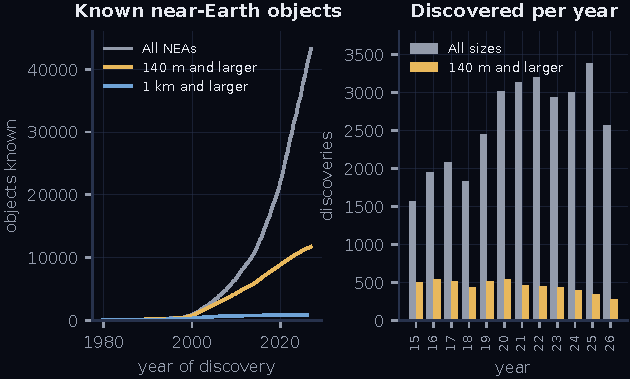
\includegraphics[width=\textwidth]{../figures/fig_catalogue.pdf}
\caption{The cumulative catalogue of known near-Earth objects by size class,
and the annual discovery rate. The kilometre class is essentially complete;
the 140-metre class is closing; the sub-140-metre population is still
arriving at three thousand a year. Source: NASA CNEOS discovery statistics,
data current 22 November 2026.}
\label{fig:catalogue}
\end{figure}

The asymmetry in \figref{fig:catalogue} is the first thing the reader should
take from it. The catalogue is nearly complete at the top and still growing at
the bottom, which means that the objects that can destroy a city are already,
for the most part, known. The problem is not that we are failing to find the
dangerous ones. The problem is that we know they are there and we do not
know what they are.

\section{What is missing, and why each thing is missing}

The missing quantities are missing for different reasons, and the differences
matter, because a measurement that is merely difficult is a different
procurement problem from a measurement that is impossible.

The \emph{size} is missing because the object is unresolved. Its brightness is
recorded and its size is not, because converting one to the other requires an
albedo\idx{Albedo}, and the albedo\idx{Albedo} is a function of composition, and composition has to be
measured. This is the degeneracy that Chapter 6 takes apart in full. The
\emph{mass} is missing because mass requires either a dynamical measurement
--- an orbit disturbed by the object itself, which for a small body means a
close approach to something massive --- or a volume and a density, and the
density is itself uncertain by a factor of about three between a rubble pile
and a monolith.

The \emph{shape} is missing because resolving a sixty-metre object at a
hundredth of an astronomical unit demands either proximity or an aperture that
nobody owns. The \emph{spin state} is missing for a different reason: it is
the easiest of the missing quantities to obtain, because a lightcurve is
cheap, and it is still missing for most objects simply because nobody has
pointed a telescope at them for long enough.

\section{Two chains through one measurement}

What follows from this inventory is the structural observation that organises
the rest of the book. The two things a defender needs are an energy and a
probability. Each of those is computed from the same physical inputs, by
chains that run in different directions but share their first link.

\begin{table}[!htbp]
\centering
\footnotesize
\caption{The two chains through the shape measurement. The right column is the
measurement that closes each link.}
\label{tab:chains}
\begin{tabularx}{\textwidth}{@{}P{0.64in}P{1.08in}YY@{}}
\toprule
\rowcolor{panel}
\textbf{Chain} & \textbf{Link} & \textbf{What limits it} & \textbf{What closes it} \\
\midrule
Accounting & Shape to volume & unknown scale & resolved imaging, or thermal flux \\
\rowcolor{panel}
 & Volume to mass & rubble pile against monolith & radar, flyby, thermal inertia \\
 & Mass to energy & \(\delta\ln E = 3\,\delta\ln D + \delta\ln \rho\) &
 diameter\idx{Diameter} to about 14 per cent \\
\rowcolor{panel}
 & Energy to hazard class & the Torino scale boundaries &
 diameter\idx{Diameter} and density together \\
Probability & Shape to YORP torque & surface normals and roughness &
 resolved shape \\
\rowcolor{panel}
 & Torque to spin state & pole known only to tens of degrees &
 lightcurve with a resolved shape \\
 & Spin state to Yarkovsky drift & thermal inertia unknown by an order of
 magnitude & thermal spectroscopy \\
\rowcolor{panel}
 & Drift to keyhole & along-track position at the horizon &
 everything above \\
\bottomrule
\end{tabularx}
\end{table}

\tabref{tab:chains} is the book's whole argument in one table. The
\emph{accounting} chain runs shape to volume to mass to energy to hazard
class. The \emph{probability} chain runs shape to YORP torque to spin state to
Yarkovsky drift to along-track displacement to keyhole. They are ordinarily
treated as separate problems, because they are owned by different programmes:
one is a sizing problem and the other is an orbit-determination problem. But
the first link of both is the same observation, made by the same instrument,
on the same body, at the same time. A resolved image of a rotating asteroid
does both jobs.

\section{Shape as the centre of gravity}

This is why the book is organised around shape rather than around ranging,
despite the owner's original instinct toward a ranging beam to Earth, and
despite the fact that ranging is the more familiar planetary-defence
activity. A range measurement tells you how far away an object is. A shape
measurement tells you how far away it is \emph{and} what it is made of, and
it feeds two chains instead of one.

There is a second reason, and it is quantitative rather than editorial. The
probability chain's sensitivity to physical error is not uniform across
horizons: at seven years the astrometric term dominates the impact
probability by three orders of magnitude, and at thirty years the physical
term dominates it by two or three. The measurement that matters is therefore
not the one that is always needed but the one that is needed at the horizon
where the physics has overtaken the astrometry. Chapter 14 works that out
with published numbers, and Chapter 30 turns it into the rule that decides
which platform to use.

\begin{keytakeaways}
\item The catalogue holds 43,212 near-Earth objects, 11,725 of them larger
than about 140 metres, and the dangerous ones are already mostly found.
\item A catalogue entry carries no size, mass, shape, spin state or density,
and each is missing for a different reason.
\item The accounting chain and the probability chain share their first link:
the resolved shape.
\item Because the physical term only overtakes the astrometric term at long
horizons, the measurement is needed selectively rather than routinely.
\end{keytakeaways}

% =====================================================================
%  Chapter 2 — The Two Axes of the Hazard Scale
% =====================================================================

\chapter{The Two Axes of the Hazard Scale}
\label{ch:two-axes}

The Torino Impact Hazard Scale, adopted by the International Astronomical Union
in 1999, is the instrument the planetary-defence community uses to say how
much attention an object deserves. It is worth reading carefully, because the
reading is where the accountability gap becomes visible.

The scale is defined on two axes. The horizontal axis is the probability
\(p\) that the object will strike Earth. The vertical axis is the kinetic
energy \(E\) the object would release, measured in megatons of TNT. Every
assignment of a level to an object is a statement about the pair \((p, E)\),
and the pair matters more than either number alone: an object with a
probability of one in ten thousand and an energy of a kiloton is a different
problem from an object with the same probability and an energy of a hundred
megatons.

\section{Why the energy axis is the hard one}

The probability axis is measured. An orbit is fitted from astrometry, the
orbit is propagated, and the probability of intersection with the Earth's
cross-section is computed. The machinery is good, the observation times are
dense, and the numerical work is unremarkable. The energy axis is inferred,
and the inference has two stages.

The first stage is the diameter. A celestial body's absolute magnitude \(H\)
and its geometric albedo \(p\) are related to its effective diameter \(D\) by
the standard relation
\begin{equation}
D = \frac{1329}{\sqrt{p}}\,10^{-H/5}\ \ \mathrm{km},
\label{eq:hdp}
\end{equation}
which is a statement that a brighter object of the same albedo is bigger.
The problem is that \(p\) is a composition measurement, and the small
near-Earth objects that matter most have had their composition measured for
about fifteen per cent of them.

The second stage is the density. The mass is \(m = \rho \pi D^{3}/6\) for a
sphere of the given diameter, and the kinetic energy at impact speed \(v\) is
\begin{equation}
E = \frac{1}{2}\,m\,v^{2} = \frac{1}{2}\,\rho\,\frac{\pi}{6}\,D^{3}\,v^{2}.
\label{eq:energy}
\end{equation}
For a near-Earth object at a typical impact speed of 14 to 17 kilometres per
second, the density\idx{Density} is the dominant uncertainty. A rubble pile with a bulk
density\idx{Density} of 1,300~kg\,m\(^{-3}\) and a coherent monolith at 3,500~kg\,m\(^{-3}\)
differ by a factor of 2.7 in mass at the same diameter, and a factor of 2.7 in
energy.

\section{The error budget, in one line}

Differentiating \eqref{eq:energy} in logarithms gives the relation the whole
book turns on:
\begin{equation}
\delta\ln E = 3\,\delta\ln D + \delta\ln \rho.
\label{eq:dlne}
\end{equation}
The diameter enters three times because volume goes as the cube. This has a
plain consequence. If the energy is to be known to within a factor of three
and the density\idx{Density} to within thirty per cent, then the diameter must be known to
within thirty per cent. If the energy is to be known to within a factor of
two, the diameter must be known to about fourteen per cent.

\begin{table}[!htbp]
\centering
\small
\caption{What diameter accuracy the energy chain demands. The density is held
at thirty per cent, which is the state of the art for the near-Earth class.}
\label{tab:diameter-need}
\begin{tabularx}{\textwidth}{@{}P{1.19in}P{1.37in}Y@{}}
\toprule
\rowcolor{panel}
\textbf{Energy known to} & \textbf{Diameter must be known to} &
\textbf{Where that stands} \\
\midrule
a factor of 3 & 30 per cent & the present state of the art \\
\rowcolor{panel}
a factor of 2 & 14 per cent & beyond the published state of the art \\
a factor of 1.5 & 7 per cent & well beyond it \\
\bottomrule
\end{tabularx}
\end{table}

The NASA Center for Near Earth Object Studies' impact monitoring service
states the position in its own terms: the tabulated impact energy\idx{Impact energy} is
``generally good to within a factor of three'', and it attributes this to mass
uncertainty dominating the budget. That is the honest characterisation of the
field's present position, and it is the number the rest of this book is trying
to move.

\section{The threshold that moves when the size moves}

The \idxw{Torino scale}'s Level 1 boundary is not a fixed probability. It is a line
in the \((p, E)\) plane, and the line's intercept depends on the energy:
\begin{equation}
p \geq \frac{10^{-7/3}}{E} = \frac{4.64\times 10^{-3}}{E}\qquad (E \text{ in Mt}).
\label{eq:level1}
\end{equation}
This follows directly from the scale's definition: Level 1 is entered when
the combination \((\log_{10} E + \tfrac{1}{3} + \log_{10} p + 2)/2\) reaches
zero.

The consequence is the single most uncomfortable fact in this chapter. An
object whose astrometry has not changed at all --- not by one milliarcsecond,
not by one orbit --- can be Level 0 or Level 1 purely because of how it was
sized. A factor of 4.5 in energy moves the Level 1 probability threshold by
the same factor of 4.5, from about \(4.7\times 10^{-4}\) to about
\(2.2\times 10^{-3}\). Whether an object is a Level 1 event, and therefore
whether it generates a formal notification through the international warning
network, is a decision made by an assumption about the object's composition.

\section{What the scale does not do}

It is worth being clear about what the scale is for, because the gap this
book describes is not a failure of the scale. The Torino scale\idx{Torino scale} is a
communication instrument. It exists to let a duty officer, a news desk and a
commissioning agency talk about the same object in the same terms. It is
doing that job.

What it cannot do is supply the energy. The scale is handed a number and
reports a level; the number arrives from the same inference described above,
and the inference is where the uncertainty lives. The scale's own structure
makes the point: it is a two-axis system in which one axis is measured to
high precision and the other is assumed. Chapter 5 works through a case in
which the assumed axis moved by a factor of 4.5 while the measured axis stood
still.

\begin{keytakeaways}
\item The Torino scale\idx{Torino scale}'s two axes are not equally supported: probability is
measured and energy is inferred.
\item The relation \(\delta\ln E = 3\,\delta\ln D + \delta\ln \rho\) makes
the diameter the dominant term, so a factor of two in energy needs a
fourteen per cent diameter.
\item The Level 1 probability threshold is proportional to the inverse of the
energy, so a mis-sized object can cross a notification boundary with its
astrometry untouched.
\item The scale is a communication instrument and is not at fault; the
uncertainty enters before the scale is applied.
\end{keytakeaways}

% =====================================================================
%  Chapter 3 — The Detection Mandate Against the Characterisation Mandate
% =====================================================================

\chapter{The Detection Mandate Against the Characterisation Mandate}
\label{ch:mandates}

Two mandates sit inside the planetary-defence establishment, and they are
funded, staffed and organised separately. The first is to \emph{find}
near-Earth objects. The second is to \emph{characterise} them. Almost all of
the hardware, almost all of the observing time and almost all of the
public attention are on the first side of that line. The second side has no
automated trigger at all.

That is not a criticism of the discovery effort, which has been extraordinarily
successful. It is an observation about where the residual risk sits once the
catalogue is built.

\section{Five clocks, not one}

The phrase "before it is too late" implies a single clock. There are five, and
they run at very different rates.

\begin{table}[!htbp]
\centering
\small
\caption{The warning-time chain, and the part of it a lunar surface station
would touch.}
\label{tab:clocks}
\begin{tabularx}{\textwidth}{@{}P{0.72in}P{1.12in}P{0.87in}Y@{}}
\toprule
\rowcolor{panel}
\textbf{Stage} & \textbf{Instrument} & \textbf{Clock} & \textbf{Lunar help} \\
\midrule
1. Discovery & wide-field optical survey & minutes of alert & partly: near-Sun
access \\
\rowcolor{panel}
2. Orbit and impact probability & astrometry, B-plane & weeks to years & yes: a
second geometry \\
3. Characterisation & spectra, radar shape, rotation, mass & the bottleneck &
yes, and most \\
\rowcolor{panel}
4. Mitigation decision & modelling & years & no \\
5. Deflection & spacecraft & years & no \\
\bottomrule
\end{tabularx}
\end{table}

Stage 1 is measured in minutes: the alert fires when the survey's astrometric
solution is good enough for a follow-up to be scheduled. Stage 2 is measured
in weeks for a short-arc object and in years for one that will return, and it
is the stage at which the astrometric term dominates for most of the
relevant horizon. Stage 3 has no fixed clock at all, because it has no
trigger: it happens when an observer with an idle telescope and an interest
happens to be pointed at the right object. Stage 4 and stage 5 are outside
this book's scope, which is deliberate; the endpoint here is accountability,
not deflection.

\section{The trigger that does not exist}

The most consequential sentence in the 2025 NASA documentation on the
2024~YR4 episode is a negative one. The planetary-defence coordination
office and the international warning network were recorded as discussing the
creation of an automated system, and the documented position was that
\textbf{no automated system currently alerts physical characterization
sites}.

The operational consequence was observed in real time. Observers at the
Infrared Telescope Facility had not learned of the object's Torino Level 1
status when they were observing it. That is, in the most literal sense, a
failure to detect: the object was detected, imaged and measured, and the
people doing so were not in the loop that would have told them the
measurement mattered.

The same documentation records that an automated alert was exercised
successfully for a Torino Level 1 event --- 2025~FA22, on 25 April 2025 ---
which establishes that the trigger is operationally simple rather than
technically difficult. The 2024~YR4 episode was therefore not a sensing
failure and not a data-processing failure. It was a routing failure.

\begin{seamnote}{A sensor does not fix a routing failure}
The owner's original concept carried a beam to Earth, and the instinct behind
it was good: a link from the risk list to an instrument that can respond. The
2024~YR4 record says the link was the missing piece, and that an automated
alert to a characterisation site is the concrete form that the link should
take. This book therefore treats the beam as an alerting\idx{Alerting} and scheduling path
rather than as a ranging channel, because the ranging channel turns out to be
the weaker claim of the two.
\end{seamnote}

\section{Where the Sun-ward blind zone bites}

Stage 1 is not equally accessible from the ground. A ground telescope cannot
observe close to the Sun: the atmospheric scattering and the sky background
rise, and the solar avoidance constraints tighten. Objects arriving from the
Sun-ward direction are therefore found late or not at all, and this is not a
hypothetical concern. The 2026 study of near-Earth-object telescopes for
extreme environments names the historical failures directly: 2008~TC3 and
2019~OK, and ``multiple other NEAs detected only days before their closest
approach to Earth''.

The geometry of that disadvantage can be inverted from the published table in
that study. For a relative velocity of 20~kilometres per second, a 140-metre
object becomes detectable from a lunar observatory at 0.10 astronomical units
and about nine days earlier than from the ground; a 30-metre object at
0.05~astronomical units and four to five days earlier; and a one-kilometre
object at 0.50~astronomical units and about six weeks earlier. Working
backwards from the lead times gives the ground limits the table implies:
about 0.20 astronomical units for the 140-metre class, about 0.10 for the
30-metre class and about 0.99 for the kilometre class.

Those are the numbers in \figref{fig:sunward} of Chapter 26, and they are the
discovery-side case for a lunar platform. The lead times are modest, and the
book does not inflate them. Their significance is not their length but their
direction: they are the only entry in the table that applies to objects the
ground structurally cannot reach.

\begin{keytakeaways}
\item The two mandates are separately funded and separately staffed, and only
one of them has a trigger.
\item The documented 2024 YR4 failure was a routing failure: the observers
were not told the object had reached Level 1.
\item An automated alert to a characterisation site was exercised
successfully for 2025 FA22 on 25 April 2025, so the missing link is
operationally simple.
\item The stage that actually binds is characterisation, and the Sun-ward
blind zone is the one part of discovery that a lunar vantage reaches and the
ground does not.
\end{keytakeaways}

% =====================================================================
%  Chapter 4 — The \idxw{Population} We Are Accountable For
% =====================================================================

\chapter{The Population We Are Accountable For}
\label{ch:population}

A programme that cannot say what it is trying to cover cannot be managed,
because it has no denominator. This chapter fixes the denominator, and in
doing so it produces the single most important number in the book: for the
class of objects that can destroy a city, the near-Earth object catalogue is
essentially complete, and the gap is not discovery. It is accounting.

\section{The three populations}

The catalogue is usually quoted as one number, 43,212 known near-Earth objects
as of 22 November 2026. That number is a poor management unit, because it
mixes objects that can level a city with objects that are less likely to
damage a building. Three populations matter, and they are worth separating.

\begin{table}[!htbp]
\centering
\small
\caption{The catalogue by the population that matters, with the annual arrival
rate. Source: NASA CNEOS discovery statistics, data current 22 November 2026.}
\label{tab:populations}
\begin{tabularx}{\textwidth}{@{}P{1.11in}P{0.73in}P{0.87in}Y@{}}
\toprule
\rowcolor{panel}
\textbf{Population} & \textbf{Known} & \textbf{Arriving} & \textbf{What it means} \\
\midrule
All near-Earth objects & 43,212 & 3,383 a year & dominated by objects too
small to matter \\
\rowcolor{panel}
140 m and larger & 11,725 & 342 a year & the population\idx{Population} a defender is
accountable for \\
1 km and larger & 883 & 2 a year & essentially complete \\
\bottomrule
\end{tabularx}
\end{table}

The 140-metre class is the working population\idx{Population}, and the choice of 140~metres is
not arbitrary. It is the size at which an object delivers enough energy to
destroy a city on its own, and it is also the threshold the discovery
statistics themselves use. The class contains 11,725 objects, which is 27.1 per
cent of the whole catalogue. Its arrival rate is falling: 441 in 2022, 431 in
2023, 397 in 2024 and 342 in 2025, because the large objects are running out
and the easy ones have already been found. At that rate the remaining
undeclared population\idx{Population} of this class is small and finite.

\begin{figure}[!htbp]
\centering
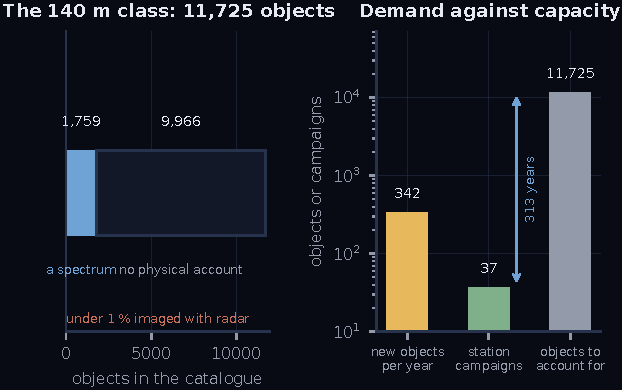
\includegraphics[width=\textwidth]{../figures/fig_accountability.pdf}
\caption{The population that is catalogued but not accounted for, and the
demand against which a single characterisation station's capacity has to be
read. The right-hand panel is logarithmic: the backlog is three hundred times
the station's annual service rate.}
\label{fig:accountability}
\end{figure}

\section{How many of them have an account}

The characterisation\idx{Characterisation} record for this population is thin. The survey of the
field's characterisation\idx{Characterisation} capability records that only about fifteen per cent
of near-Earth objects have had a spectrum measured, and that fewer than one
per cent have been imaged with radar. Applied to the 140-metre class, those
two figures give about 1,759 objects with a spectrum and fewer than about 120
with a radar image. The remainder, about 9,966 objects, have no physical
account at all.

\begin{table}[!htbp]
\centering
\small
\caption{The physical accounts that exist for the 140-metre class, as far as
the published figures reach.}
\label{tab:accounts}
\begin{tabularx}{\textwidth}{@{}P{1.60in}P{0.96in}Y@{}}
\toprule
\rowcolor{panel}
\textbf{Account} & \textbf{Objects} & \textbf{What it settles} \\
\midrule
A spectrum & about 1,759 & composition, taxonomy, and an albedo prior \\
\rowcolor{panel}
A radar image & fewer than about 120 & shape, spin state, and in principle
mass \\
A resolved shape model & a few dozen & the volume that the energy chain
starts from \\
\rowcolor{panel}
A mass & very few & the density, and with it the last term in
\eqref{eq:dlne} \\
\bottomrule
\end{tabularx}
\end{table}

The last row is the one that should worry a programme manager most. A
resolved shape model gives the volume; the mass gives the density; the
density is the other factor of three in \eqref{eq:dlne}. A catalogue in which
one object in seven has a spectrum and one in a hundred has a radar image is
not a catalogue of known threats. It is a catalogue of known objects.

\section{The managerial consequence}

The arithmetic in the previous three sections produces a conclusion that
determines the shape of the whole proposal, and it is a conclusion about
\emph{what kind of thing} the capability should be.

If the gap were a discovery gap, the right response would be more survey
capacity: a larger aperture, a longer telescope, a faster cadence. The
published survey record shows that the discovery side is not the bottleneck
for the class that matters. The 140-metre population is nearly complete in
discovery and nearly untouched in characterisation. Building more survey
capacity adds objects to a queue that already cannot be served.

If the gap were a capacity gap --- if there were simply too many objects to
characterise for any instrument to keep up --- then the response would be to
build a census machine and accept the cost. It would not be a census machine,
because the arithmetic rules it out. A fixed station needs a 90-degree sweep
of its baseline orientation to deliver the two orthogonal measurements an
interferometric position requires, and the Moon's rotation takes 6.83 days
to deliver that sweep. Allowing thirty per cent of the time for overhead, one
station runs about 37 campaigns a year. Against an arrival rate of 342
objects a year for the hazard class, that is 10.9 per cent of the flow, and
against the 11,725 known objects it is a clearance time of 313 years.

\begin{keytakeaways}
\item The working population is the 11,725 known objects larger than about
140 metres, and its discovery is essentially complete.
\item About 1,759 have a spectrum, fewer than about 120 have a radar image,
and about 9,966 have no physical account at all.
\item More survey capacity would add objects to a queue that cannot be served;
the bottleneck is characterisation\idx{Characterisation}, not detection.
\item One station runs about 37 campaigns a year, which is 10.9 per cent of
the annual flow and a 313-year clearance of the known catalogue, so the
capability must be a triage and not a census.
\end{keytakeaways}

The conclusion follows directly, and it is the load-bearing structural claim of
the book: \textbf{for the hazard class, the gap is accounting, not
discovery}. A capability for this population therefore cannot be justified by
how much it finds, and it cannot be justified by the size of the backlog.
It has to be justified by the decisions it changes --- which is to say, by the
objects whose characterisation actually alters an outcome. That is a
narrower claim than ``characterise the catalogue'', and Chapter 30 turns it
into a rule.

\begin{figure}[!htbp]
\centering
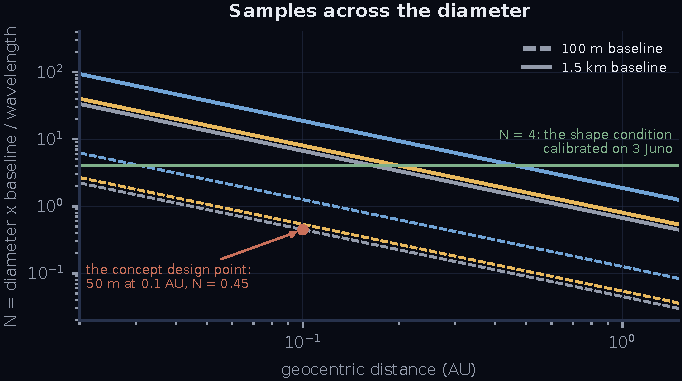
\includegraphics[width=\textwidth]{../figures/fig_samples.pdf}
\caption{Samples across the diameter against baseline and distance. A single
100-metre baseline never reaches four samples for the 50-metre class at
0.2 astronomical units, and the proposed array is what closes the gap.}
\label{fig:samples}
\end{figure}

% =====================================================================
%  Chapter 5 — \idxw{2024 YR4}: The Case Where the Response Failed
% =====================================================================

\chapter{2024 YR4: The Case Where the Response Failed}
\label{ch:yr4}

One object has been studied hard enough to expose every part of the problem
this book describes. It was discovered on the night of a close approach, it
was sized three different ways that disagree by a factor of 1.7 in diameter,
it is due to hit the Moon in 2032, and it has a formal warning attached to it
that is generated by a scale whose energy axis rests on those disagreeing
sizes.

The record is unusually complete, and it is worth reading closely because
almost every number in this book was checked against it.

\section{How it was found}

The JPL Small-Body Database records the first observation of 2024~YR4 on
25 December 2024. The close-approach record for the same date gives the
distance: 0.00554 astronomical units, or 828,775 kilometres, at a relative
velocity of 13.75 kilometres per second.

So the object was discovered on the very night it passed inside the Earth's
sphere of influence, at a distance of roughly five and a half lunar
distances. That is a discovery with almost no warning attached, and it is
worth noting that it was nonetheless a success: the object was found at
all, and its orbit was good enough that the 2032 lunar encounter could be
computed at all.

The orbit solution is not marginal. It uses 485 observations with a residual
of 0.45 arcseconds, and the absolute magnitude it carries is
\(23.93 \pm 0.28\). That last figure is worth holding on to, because the
2025 \idxw{JWST} analysis of the object gives \(24.14 \pm 0.25\), which is a
discrepancy of 0.21 magnitudes --- inside both uncertainties, and therefore
the sort of difference that ought not to change anything. It is carried
through this book rather than reconciled, because a reader checking the
catalogue against the literature should be able to see that the two agree as
well as they do.

\section{Three sizes, one object}

The 26 March 2025 JWST\idx{JWST} MIRI analysis is the most thorough physical
characterisation of any object of this class, and it is a study in the
degeneracy the earlier chapters described. The measurements it reports are
the following: a spin pole at galactic coordinates \((l, b) = (232^\circ,
-11^\circ)\); a sidereal rotation period of 19.4633 minutes; axis ratios
\(a/b \approx 1.28\) and \(b/c \approx 1.45\); an equivalent-volume diameter
of 60.8 metres with an uncertainty of \(+1.8\) and \(-3.6\) metres; a
geometric albedo of \(0.11^{+0.05}_{-0.03}\) from the absolute magnitude
\(H_V = 24.14 \pm 0.25\); and a high thermal inertia with low surface
roughness.

Those are excellent numbers. The difficulty is that the object has not been
measured, and the size comes from a thermal model whose assumptions are
being fitted rather than tested.

\begin{table}[!htbp]
\centering
\small
\caption{The three thermal models in the published analysis of 2024 YR4, and
what each gives for the diameter.}
\label{tab:yr4-models}
\begin{tabularx}{\textwidth}{@{}P{1.65in}P{0.91in}Y@{}}
\toprule
\rowcolor{panel}
\textbf{Model} & \textbf{Diameter} & \textbf{Note} \\
\midrule
NEATM, standard & 60.6 m & requires a beaming parameter\idx{Beaming parameter} of 3.06, which is
unphysical, and is rejected \\
\rowcolor{panel}
Fast rotating model & 51.1 m & albedo 0.16 \\
\idxw{Thermophysical model} & 60.8 m & the published best fit \\
\bottomrule
\end{tabularx}
\end{table}

The two credible models differ by 19 per cent in diameter. Because volume
goes as the cube, that is a factor of 1.68 in energy at fixed density. The
object's physical description is therefore uncertain at the 20 per cent level
for a reason that has nothing to do with the quality of the observations and
everything to do with the choice of model.

\section{What that does to the hazard class}

Carried through \eqref{eq:energy} at the published lunar-impact speed of
14.1 kilometres per second and across the density range from a rubble pile
at 1,300 to a coherent body at 3,500 kilogrammes per cubic metre, the
published model set spans 2.16 to 9.79 megatons --- a factor of 4.5.

The decomposition is exact and it is the most useful single calculation in
this chapter. The thermal-model choice alone contributes a factor of
\((60.8/51.1)^3 = 1.68\), and the density choice alone contributes
\(3500/1300 = 2.69\). Their product is 4.53, against the published spread of
4.53. Two thirds of the uncertainty in the energy is a modelling choice; one
third is a composition assumption. Neither is an observational error.

\begin{figure}[!htbp]
\centering
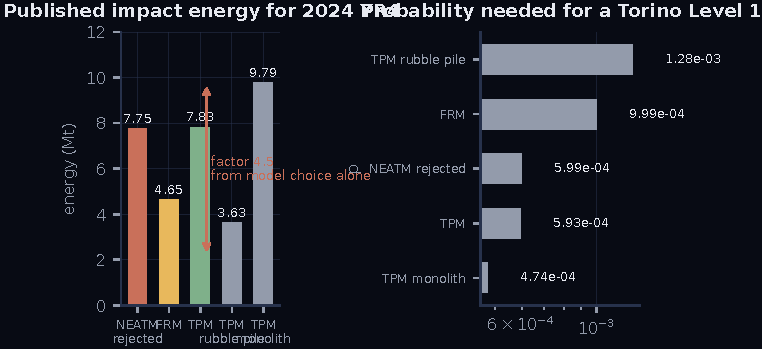
\includegraphics[width=\textwidth]{../figures/fig_yr4.pdf}
\caption{Left: the impact energy of 2024 YR4 under the published model set.
Right: the probability required for a Torino Level 1, which moves with the
energy. The astrometry is identical in every case.}
\label{fig:yr4}
\end{figure}

Now apply \eqref{eq:level1}. The Level 1 threshold probability for this object
is \(4.64\times 10^{-3}/E\), so the threshold ranges from \(4.7\times 10^{-4}\)
at 9.79 megatons to \(2.2\times 10^{-3}\) at 2.16 megatons. An object whose
orbit has not moved by a milliarcsecond can be Level 0 or Level 1 on the
strength of a modelling decision.

That is the accountability gap expressed as a single number, and it is why
the book's endpoint is accountability rather than detection.

\section{The encounter, and what it would have measured}

The object's next close approach is on 22 December 2032, at 0.00186
astronomical units or 278,333 kilometres from the Earth's centre. That
approach ends in an impact on the Moon, and the published accounts of it
disagree in a way that must be carried rather than reconciled: the JWST\idx{JWST}
analysis reports a lunar passage within \(22,900 \pm 800\) kilometres, while
the independent Monte Carlo study reports a nominal selenocentric closest
approach of 3,000 kilometres with a lunar B-plane uncertainty of 25,000
kilometres and 426 of 10,000 clones striking the Moon, giving 4.26 per cent;
the ejecta analysis uses 4 per cent. The difference is between a
closest-approach statistic weighted over the impact-probability distribution
and the nominal trajectory of a specific solution.

What matters for this book is what the geometry would allow a measurement to
do. At 22,900 kilometres a 60.8-metre object subtends 548 milliarcseconds,
which a 0.35-metre aperture resolves and a matched interferometric baseline
of 1.13 metres images with four samples across the diameter. At the
nominal 3,000-kilometre distance it subtends 4.18 arcseconds and the matched
baseline is 0.15 metres. In both cases the range is not inferred from an
orbit at all: the Moon's own ephemeris gives it directly, to the centimetre.

\section{The 2028 apparition, and the limit of the argument}

Between the 2024 discovery and the 2032 encounter, the object's only
opportunity is the 2028 apparition, an Earth encounter at 0.05 astronomical
units, where it is about 17.4 magnitudes and 1.68 milliarcseconds across.

This is where the book's argument must be careful, because a reader is
entitled to know what the lunar platform would and would not have bought.
The 2025 to 2028 interval was a \emph{distance} problem: the object was too
far from the Earth for any observatory to do useful work on it, and no
vantage point fixes that. And at 0.05 astronomical units the object is
unresolved and 1.68 milliarcseconds across, so a lunar station would have
measured its position, not its shape.

What the 2032 encounter offers is different and better: a resolved image at
short range, and a range that is known rather than fitted. The prediction the
book makes is therefore modest and falsifiable. With a lunar surface array,
the 2032 apparition would yield a resolved shape and a pole for 2024~YR4
from a range of 3,000 to 23,000 kilometres, and the shape would supply the
volume that the three thermal models cannot agree on. Without one, the shape
of 2024~YR4 will continue to be inferred from a convex lightcurve inversion
and a single thermal campaign, and the energy will remain uncertain by a
factor of about two.

\begin{keytakeaways}
\item 2024 YR4\idx{2024 YR4} was discovered on the night it passed at 828,775 kilometres,
and its 2032 encounter ends in an impact on the Moon.
\item Two credible thermal models differ by 19 per cent in diameter, which is
a factor of 1.68 in energy and nothing to do with the observations.
\item The energy spread of 4.5 decomposes exactly into 1.68 from the thermal
model and 2.69 from the density.
\item The Level 1 probability threshold moves from \(4.7\times10^{-4}\) to
\(2.2\times10^{-3}\) across that spread, with the astrometry untouched.
\end{keytakeaways}


\part{The Physics of Accountability}
\label{part:physics}
% =====================================================================
%  Chapter 6 — Size Conventions and the Albedo-Temperature Degeneracy
% =====================================================================

\chapter{Size Conventions and the Albedo-Temperature Degeneracy}
\label{ch:size-conventions}

Before the energy of an impact can be computed, the size of the object has to
be fixed, and fixing the size of a small body is harder than it looks. This
chapter works through the two available routes to a diameter --- the
reflected-light route and the thermal route --- and shows that each carries an
assumption that is not measured. The degeneracy is not a defect of the
instruments. It is a property of the information available.

\section{The absolute magnitude and what it means}

A body's absolute magnitude \(H\) is the magnitude it would have at one
astronomical unit from the Sun and one astronomical unit from the observer,
at zero phase angle. It is a measure of the reflected light the body would
return if it were seen under standard conditions, and it is the only
photometric quantity the catalogue reliably carries.

The relation between \(H\), the geometric albedo \(p\) and the effective
diameter \(D\) is
\begin{equation}
D = \frac{1329}{\sqrt{p}}\,10^{-H/5}\ \ \mathrm{km},
\label{eq:hdp2}
\end{equation}
which follows from the definition of the albedo and the geometry of the
diffuse-reflection approximation. For a body of a given albedo, the diameter
is set by the brightness; for a body of a given brightness, the diameter is
set by the albedo.

The albedo is a composition measurement. A dark carbonaceous surface reflects
a few per cent; a bright silicate surface reflects several tens of per cent.
Changing the assumed albedo from 0.10 to 0.20 changes the diameter by a
factor of \(1/\sqrt{2}\), which is a factor of \(2.8\) in volume and a factor
of \(2.8\) in mass.

That is already a large effect, and it is only the first of two.

\section{The thermal route, and the beaming parameter}

The second route measures the body's own heat. A small body absorbs sunlight
and reradiates it, and the flux it emits in the thermal infrared is a
function of its temperature, its emissivity and its projected area --- which
is a function of its diameter.

The equilibrium temperature\idx{Equilibrium temperature} follows from a balance. The absorbed flux at
heliocentric distance \(r\), for a body with geometric albedo \(A\) and
emissivity \(\varepsilon\), is \((1-A)S_0/r^{2}\) per unit area, where \(S_0\)
is the solar constant at one astronomical unit. The emitted flux is
\(\varepsilon\sigma T^{4}\). Balancing them and inserting the solar constant
gives the familiar result
\begin{equation}
T_{\mathrm{eq}} = 278\ \mathrm{K}\ \left(\frac{1\ \mathrm{AU}}{r}\right)^{1/2}
\label{eq:teq}
\end{equation}
for \(A = 0.1\) and \(\varepsilon = 0.9\), and a factor \(((1-A)/\varepsilon)^{1/4}\)
for other values. The temperature does not depend on the size, which is the
reason the technique works.

The observed flux, however, does. The total thermal flux from a body of
diameter \(D\) is proportional to \(D^{2}\), and the relationship between the
observed flux and the body's own emission depends on how the heat is
distributed over the surface. That distribution is summarised by the
\emph{beaming parameter} \(\eta\): it is the ratio of the total emitted power
to the power that a smooth sphere would emit at the same subsolar
temperature. For a body whose surface radiates efficiently the beaming
parameter approaches unity; for a rough surface with self-shadowing it is
smaller. The physically allowed range is \(0 < \eta \leq 1\).

The observed flux therefore scales as
\begin{equation}
F_{\mathrm{obs}} \propto \eta\,D^{2},
\label{eq:eta}
\end{equation}
and \eqref{eq:eta} is the degeneracy. The diameter and the beaming parameter
cannot be separated by a single thermal band: the measurement determines the
product, and the diameter is fixed only by assuming a beaming parameter.

\section{What the beaming parameter costs, and how it is detected}

The assumption is testable, because a beaming parameter above unity is
unphysical, and a fit that returns one is telling you that the model is
wrong rather than that the object is strange. The 2025 JWST analysis of
2024~YR4 is an exact illustration.

\begin{table}[!htbp]
\centering
\small
\caption{The three thermal models fitted to 2024 YR4, and what the beaming
parameter did to each.}
\label{tab:thermal-models}
\begin{tabularx}{\textwidth}{@{}P{1.14in}P{0.74in}P{0.82in}Y@{}}
\toprule
\rowcolor{panel}
\textbf{Model} & \textbf{Diameter} & \textbf{Albedo} & \textbf{Status} \\
\midrule
NEATM, standard & 60.6 m & --- & requires a beaming parameter of 3.06,
which is unphysical; rejected \\
\rowcolor{panel}
Fast rotating model & 51.1 m & 0.16 & a coherent rotation model, credible \\
Thermophysical model & 60.8 m & --- & the published best fit; a
non-rotating body with a thermal inertia\idx{Thermal inertia} \\
\bottomrule
\end{tabularx}
\end{table}

The two credible models differ by 19 per cent in diameter: 51.1 against
60.8 metres. The photometry\idx{Photometry} that produced them is excellent. The difference
between them is entirely a statement about how the heat is distributed, and
therefore about how the surface is shaped.

\begin{deeper}{Why the thermophysical model is not simply better}
The thermophysical model treats the body as having a finite thermal inertia\idx{Thermal inertia},
so the surface temperature varies through the rotation and the night is
cooler than the day. That is physically more realistic, and it is the source
of the high thermal inertia\idx{Thermal inertia} and low surface roughness reported for
2024~YR4. But realism in the forward model is not the same as freedom from
assumption: the thermophysical model still has to be supplied with a spin
state, a thermal inertia and a roughness distribution, and it delivers a
diameter that is 19 per cent larger than the one the coherent-rotation model
gives. The correct reading is not that one model is right. It is that the
model choice is worth more than the measurement error, and that a
measurement which does not depend on the model --- a resolved image --- is
worth a great deal.
\end{deeper}

\section{The photometric route, and its own assumption}

The third route is the one the field uses most, because it is the cheapest.
A lightcurve gives the object's rotation period and the projected extent of
its brightness variation; combined with the absolute magnitude, an inversion
produces a shape model, and from the model a volume, a diameter and an
albedo.

The assumption here is the convexity. A lightcurve constrains the body's
projected outline in two dimensions as it rotates, and the standard inversion
returns the convex hull\idx{Convex hull} of the constraint set --- a convex body, by
construction, whatever the body actually is. This is the subject of
Chapter 17.

\section{Why the degeneracy is the practical problem}

Taken together, the three routes have this structure. The photometric route
assumes convexity and returns an albedo as an output rather than an input.
The thermal route assumes a beaming parameter and cannot detect it from a
single band. The absolute magnitude route assumes an albedo and has no way
to check it.

\begin{table}[!htbp]
\centering
\small
\caption{The three routes to a diameter, the assumption each one makes, and
the size of the resulting uncertainty in the energy.}
\label{tab:routes}
\begin{tabularx}{\textwidth}{@{}P{1.36in}P{1.68in}P{1.23in}@{}}
\toprule
\rowcolor{panel}
\textbf{Route} & \textbf{Assumption} & \textbf{Energy factor} \\
\midrule
Thermal, single model & beaming parameter & 1.0, by definition \\
\rowcolor{panel}
Thermal, model spread & choice of model & 1.68 for 2024 YR4 \\
Absolute magnitude & albedo & up to 2.8 \\
\rowcolor{panel}
Photometric inversion & convexity & of order 1.1 to 1.3 \\
Resolved imaging & none of the above & bounded by the imaging \\
\bottomrule
\end{tabularx}
\end{table}

The last row is the reason this book exists. A resolved image does not need
an albedo, a beaming parameter or a convexity assumption. It reports the
projected area at the epoch, and the projected area is a measurement. What it
does not directly report is the volume, because a projection of a rotating
body is not a projection of its shape unless the body is convex --- but it
reports the two-dimensional geometry that the volume has to be built on, and
it reports it without a model.

\begin{keytakeaways}
\item A diameter cannot be obtained from photometry\idx{Photometry} without an assumption
about the albedo, and cannot be obtained from a single thermal band without
an assumption about the beaming parameter.
\item The beaming parameter is bounded by unity, so a fit returning 3.06 is a
detectable model failure rather than a measurement.
\item The two credible thermal models for 2024 YR4 differ by 19 per cent in
diameter, which is a factor of 1.68 in energy at fixed density.
\item The measured values in \tabref{tab:routes} are the model choices, and
the resolved imaging row is the only one with no model in it.
\end{keytakeaways}

% =====================================================================
%  Chapter 7 — Density, Rubble Pile\idx{Rubble pile} and Monolith
% =====================================================================

\chapter{Density, Rubble Pile and Monolith}
\label{ch:density}

The previous chapter ended with a measurement that removes the diameter
uncertainty. This chapter asks what remains, and the answer is the density:
the second factor of three in the energy relation, and the harder of the two
to obtain.

\section{Where the factor of three comes from}

A small body's bulk density is the product of its skeletal grain density and
its porosity, and its porosity is a statement about whether the body is a
coherent pile of fragments or a single bonded object. A rubble pile\idx{Rubble pile} of
fragments with the same grain density as a coherent body carries a void
fraction, and a typical void fraction of forty per cent reduces the bulk
density to three fifths of the solid value. That ratio, inverted, is the
factor of about three that separates the two populations.

The range is therefore not a measurement uncertainty in the ordinary sense.
It is a choice between two physical models of the object, and the object is
one or the other. The 2024~YR4 model set brackets it explicitly: 1,300
kilogrammes per cubic metre for a rubble pile\idx{Rubble pile} and 3,500 for a coherent body,
a ratio of 2.69, which propagates directly into the energy.

\section{How density is measured, and when}

There are four routes, and they are available at very different moments in
an object's life.

Radar polarimetry\idx{Polarimetry} measures the scattering signature of the regolith and can
distinguish a consolidated surface from a particulate one. It requires a
radar target, which in practice means proximity, and it is the most direct
surface-diagnostic of the four.

Thermal inertia measures how quickly the surface temperature responds to
insolation, and therefore how fine-grained and how loose the regolith is.
It is inferred from the shape of the thermal emission curve through a
rotation, and it constrains the regolith rather than the bulk body.

Flyby imaging measures the volume directly and the bulk density follows from
a separately determined mass. It is the most complete route and it is
available only to the handful of objects a spacecraft has visited.

The fourth route is the one this book is interested in, because it is the one
that scales: \emph{the close approach}. During an encounter inside the
gravitational sphere of influence of a massive body, the trajectory of the
object carries the imprint of that body's mass\idx{Mass}, and the imprint is
measurable.

\section{Why a close approach reveals the mass distribution}

The mechanism is subtle and it is worth stating carefully, because it is the
step that links the probability chain to the accounting chain.

An asteroid's mass\idx{Mass} and its internal mass\idx{Mass} distribution determine how it
responds to a gravitational perturbation. A spherical, rigid body and a
tumbling, elongated body with a concentrated mass distribution respond
differently to the same flyby: the same impulse along-track changes the
rotation rate of one and the rotation axis of the other, by different
amounts. The observable that changes is the spin state.

The 2022 study of Apophis's non-principal-axis rotation through its 2029
Earth encounter quantifies this. Working with refined orbit, spin-state and
inertia information from optical and radar observations, and propagating the
coupled orbital and rigid-body attitude dynamics through the encounter, it
finds that the gravitational changes to the tumbling periods and to the
rotational angular momentum direction are likely to be significant and
measurable. Apophis is likely to remain in a short-axis-mode tumbling state,
but its effective spin rate could halve or double, and its pole is likely to
shift by ten degrees or more and to move closer to the ecliptic plane. The
study is explicit that these changes are very sensitive to the close-approach
attitude and to the mass distribution --- and explicit about the
consequence: ground-based tracking of the spin state\idx{Spin state} through the encounter
will help refine the mass distribution.

That is the link. The spin state\idx{Spin state} is measurable from the ground with
photometry and a resolved shape. The mass distribution is not measurable from
the ground at all, except through the encounter. And the encounter is the one
occasion on which the mass distribution becomes observable at all.

\begin{seamnote}{This is why the shape and the density belong in one proposal}
A resolved shape measurement and a close-approach mass measurement are not
two independent capabilities that happen to be useful together. They are two
measurements of the same encounter: the shape supplies the volume, the
encounter supplies the mass, and the density is their quotient. An
architecture that can do the first and be present for the second closes the
entire energy chain, and an architecture that can do only the first closes
half of it.
\end{seamnote}

\section{What the density is worth at long horizons}

The last piece is the payoff, and it comes from the probability side of the
ledger. In the impact-probability study of Apophis's 2036 encounter, the
published sensitivity table varies one physical assumption at a time and
reports the resulting impact probability against the nominal case of
\(7.07\times 10^{-9}\).

\begin{table}[!htbp]
\centering
\small
\caption{The 2036 keyhole: the published sensitivity of the impact
probability to physical assumptions, against a nominal \(7.07\times10^{-9}\).}
\label{tab:bottke}
\begin{tabularx}{\textwidth}{@{}P{1.92in}P{1.27in}P{1.08in}@{}}
\toprule
\rowcolor{panel}
\textbf{Varied assumption} & \textbf{Impact probability} & \textbf{Factor} \\
\midrule
Nominal & \(7.07\times 10^{-9}\) & 1 \\
\rowcolor{panel}
Diameter 270 \(\pm\) 60 m & \(3.06\times 10^{-6}\) & 433 \\
Uniform \(\cos\gamma\) & \(2.67\times 10^{-9}\) & 0.38 \\
\rowcolor{panel}
Symmetric \(\cos\gamma\) & \(1.64\times 10^{-9}\) & 0.23 \\
Density variance, \(\sigma_\rho^{2} = 0.6\) & \(6.60\times 10^{-7}\) & 93 \\
\rowcolor{panel}
\(\mu_{d0} = 200\) & \(1.58\times 10^{-9}\) & 0.22 \\
\(\mu_{d0} = 400\) & \(1.59\times 10^{-8}\) & 2.25 \\
\bottomrule
\end{tabularx}
\end{table}

Two lines in \tabref{tab:bottke} carry the argument of this book. The
diameter assumption alone moves the impact probability by a factor of 433.
The density variance moves it by a factor of 93. Both are physical
assumptions, both are the kind of assumption a characterisation campaign is
designed to remove, and neither is touched by additional astrometry.

\begin{figure}[!htbp]
\centering
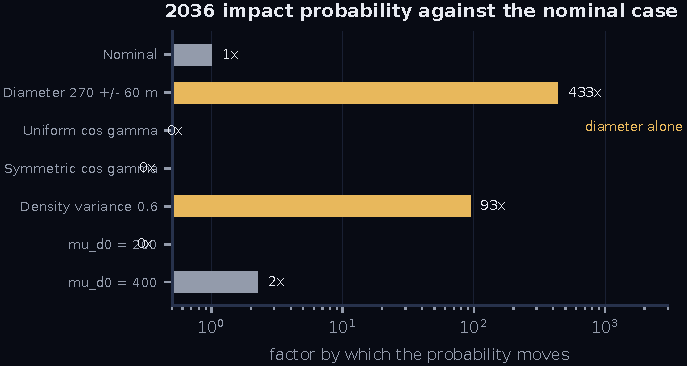
\includegraphics[width=\textwidth]{../figures/fig_keyhole.pdf}
\caption{The 2036 keyhole magnifies physical error. The diameter assumption
alone moves the impact probability by a factor of 433, and the density
variance by a factor of 93.}
\label{fig:keyhole}
\end{figure}

\figref{fig:keyhole} is the reason the book does not stop at shape. A
measurement that removes the diameter assumption removes the largest single
term in the table. A measurement that also removes the density assumption
removes the second largest. Both are attainable, both are attainable at the
same encounter, and neither is attainable by adding telescope time to an
existing programme.

\begin{keytakeaways}
\item The density range between a rubble pile and a coherent body is a factor
of about 2.7 in mass, and it is a choice between physical models rather than
a measurement noise.
\item A close approach reveals the mass distribution through its effect on
the spin state\idx{Spin state}, and the spin state is measurable from the ground.
\item The published 2029 Apophis study finds the spin rate could halve or
double and the pole could shift by ten degrees or more, and states that
tracking that change refines the mass distribution.
\item At the 2036 keyhole the density assumption is worth a factor of 93 in
the impact probability, and the diameter assumption a factor of 433.
\end{keytakeaways}

% =====================================================================
%  Chapter 8 — Shape as the Geometry \idxw{Volume} Is Built From
% =====================================================================

\chapter{Shape as the Geometry Volume Is Built From}
\label{ch:shape-geometry}

The volume\idx{Volume} of a body is not observable. What is observable is its projected
area, and the volume\idx{Volume} has to be constructed from that projection on the
assumption that the body is convex. This chapter is about that construction:
why it is unavoidable, what it costs, and what the one measurement in the
record that bypassed it actually found.

\section{Why volume cannot be observed}

A shape model is a three-dimensional object, and a shape model is not a
measurement. It is an inversion: a set of constraints on the body's
silhouette, or on its brightness as it rotates, combined with an assumed
geometry, yields a body.

The distinction matters for the energy chain, because \eqref{eq:energy} needs
a volume\idx{Volume} and not an area. The projected area of a body at a given aspect
angle is a measurement. The volume behind that projection is not. The
conversion from one to the other is the convex-hull assumption, and it is
the assumption that a resolved image cannot avoid either --- but it can
\emph{measure} it, by imaging the body from more than one aspect, or by
using the rotation to image it from many.

For a convex body, the convex hull of the projected silhouette is the body,
and the volume is exact. For a non-convex body, the convex hull is larger
than the body, and the error is one-sided: it always overstates the volume.

\section{What the record contains}

The measurement record of asteroid shapes by interferometry consists, almost
entirely, of one result, and it is worth reading in detail because it is
unique in every respect that matters.

On 15 May 2017 the asteroid (372) Palma occulted the radio galaxy
0141+268. The shadow of the asteroid crossed the Very Long Baseline Array
station at Brewster, Washington, and six \idxw{VLBA} antennas recorded it. At the
observing wavelength of 4.2 centimetres, with the asteroid's radius near
95 kilometres and its distance at 3.436 astronomical units, the Fresnel
number was 0.43 --- which means the diffraction pattern fell in the
Fraunhofer regime and was observable on the Earth.

The measurement retrieved both the amplitude and the phase of the diffracted
electromagnetic wave. It is the first astronomical measurement of the phase
shift caused by diffraction by an asteroid, and the maximum phase shift is
directly sensitive to the effective diameter.

\begin{table}[!htbp]
\centering
\small
\caption{The 2017 radio occultation of (372) Palma: what was measured and
what it returned.}
\label{tab:palma}
\begin{tabularx}{\textwidth}{@{}P{2.57in}Y@{}}
\toprule
\rowcolor{panel}
\textbf{Quantity} & \textbf{Value} \\
\midrule
Technique & radio occultation\idx{Radio occultation}, six VLBA\idx{VLBA} antennas, 4.2 cm, 6.996 GHz \\
\rowcolor{panel}
Baselines to the Brewster station & 1,200 to 2,300 km \\
\idxw{Fresnel number} & 0.43, Fraunhofer regime \\
\rowcolor{panel}
Effective diameter, all silhouette models & \(192.1 \pm 2.3\) km \\
Effective diameter, circular-disk fit & \(192.1 \pm 4.8\) km \\
\rowcolor{panel}
Maximum phase shift & \(76.4 \pm 2.5\) degrees \\
Cross-check, thermal mid-infrared & \(191.1 \pm 2.7\) km and
\(186.5 \pm 6.3\) km \\
\rowcolor{panel}
Roundness, ratio of inscribed to circumscribed circle & mean 0.866, standard
deviation 0.093 \\
Departure from a circle & 10 to 20 per cent \\
\bottomrule
\end{tabularx}
\end{table}

Three things in \tabref{tab:palma} matter for the rest of the book.

The first is the scale. The measured object is 192 kilometres across. The
class this book is about is 50 to 140 metres across, so Palma is more than
a thousand times wider in diameter and more than a billion times larger in
volume. Any statement about the feasibility of asteroid interferometry has
to be read with that ratio in mind.

The second is the shape. The silhouette is slightly elongated and has a
concave edge, and the roundness distribution --- built from 24,000 random
contiguous silhouettes fitted to the observed amplitude and phase curves ---
has a mean of 0.866 with a standard deviation of 0.093, and gives a
departure from a perfect circle of 10 to 20 per cent with the roundness
bounded below at 0.63 with ninety-five per cent confidence. The earlier
arXiv abstract of the same study gave the departure as \(26 \pm 13\) per
cent; both figures are carried here because both were published, and the
conclusion is the same either way.

The third is the epilogue. The study notes that although the more than
1,600 astrometric observations of Palma span more than 120 years, the
addition of a single radio interferometric occultation measurement had a
non-negligible effect on the uncertainties of the orbital elements and
reduced the uncertainty of the ephemerides by an order of magnitude. One
measurement, one night, and the long-term ephemeris improved by a factor of
ten. That is the character of the observation this book is proposing.

\section{The scale of the problem, restated}

\begin{figure}[!htbp]
\centering
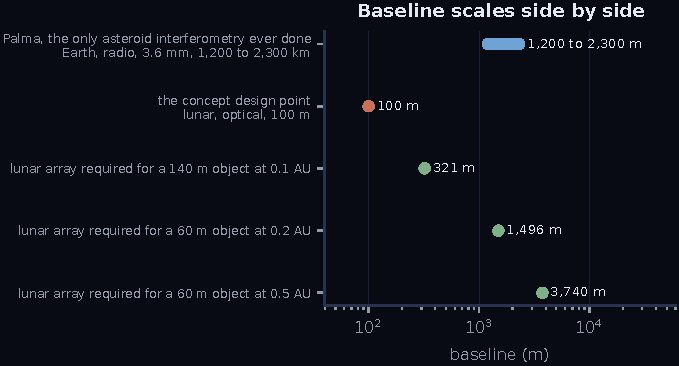
\includegraphics[width=\textwidth]{../figures/fig_scale.pdf}
\caption{Baseline scales side by side. The only asteroid interferometry ever
performed used terrestrial baselines of 1,200 to 2,300 kilometres at radio
wavelengths, on a target 192 kilometres wide. The baselines an optical
shape imager needs for the small class are one to two orders of magnitude
shorter, but they have to be held to a stability the ground cannot hold.}
\label{fig:scale}
\end{figure}

\figref{fig:scale} sets the two scales against each other, and the
comparison is deliberately framed in the most favourable way available to the
existing technique. Palma's measurement used the largest terrestrial
baselines there are, at radio wavelengths where the coherence requirements
are mild, on a target three orders of magnitude larger than the class this
book concerns, and it worked.

The optical problem is different in kind rather than in degree. A
radio-interferometric image of an unresolved body at 4.2 centimetres is
obtained by measuring the amplitude and phase of a diffraction pattern; an
optical interferometric image of a resolved body at 750 nanometres requires
the fringe visibility of a limb profile to be measurable, which requires the
baseline to be matched to the body's angular size rather than to exceed it.
Chapter 20 works through that condition, and it is the reason the concept
literature's hundred-metre baseline does not do what the book needs.

\section{What this means for the energy chain}

The chain can now be written out in the form the rest of the book uses.

\begin{table}[!htbp]
\centering
\small
\caption{From a resolved image to an energy, with the assumption at each
step made explicit.}
\label{tab:shape-to-energy}
\begin{tabularx}{\textwidth}{@{}P{1.20in}P{1.36in}Y@{}}
\toprule
\rowcolor{panel}
\textbf{Step} & \textbf{Quantity produced} & \textbf{Assumption} \\
\midrule
Resolved image & projected area at the epoch & none; this is a measurement \\
\rowcolor{panel}
Projection to volume & volume & convexity\idx{Convexity}, unless the rotation supplies
multiple aspects \\
Volume to mass & mass & bulk density \\
\rowcolor{panel}
Mass to energy & energy & impact speed, which is well determined \\
Energy to hazard class & Torino level & the scale's own definitions \\
\bottomrule
\end{tabularx}
\end{table}

The middle row is where a resolved image earns its place. It replaces a
model choice --- the thermal beaming parameter, or the convexity\idx{Convexity} of the
inversion --- with a measurement, and it is the only step in the chain that
a resolved image can close without any other instrument's help. The row
below it is the one that requires an encounter, and Chapter 7 has argued
that the same encounter supplies it.

\begin{keytakeaways}
\item A volume cannot be observed; it is constructed from a projection, and
the construction assumes convexity.
\item The convex-hull error is one-sided: it always overstates the volume.
\item The only asteroid silhouette ever measured by interferometry is
(372) Palma, by radio occultation\idx{Radio occultation} with the VLBA\idx{VLBA}, and it found a body 192
kilometres across whose silhouette departs from a circle by 10 to 20 per
cent.
\item A single such measurement reduced that object's long-term ephemeris
uncertainty by an order of magnitude.
\end{keytakeaways}

% =====================================================================
%  Chapter 9 — Spin, \idxw{Pole} and the \idxw{Lightcurve}
% =====================================================================

\chapter{Spin, Pole and the Lightcurve}
\label{ch:spin}

The spin state of a small body is the easiest of the missing quantities to
measure and the most consequential to get right. It is easy because a
lightcurve\idx{Lightcurve} is cheap: point a telescope at an object, watch it brighten and
dim. It is consequential because the spin state enters the probability chain
in two places and the accounting chain in none.

\section{What a lightcurve contains}

A rotating body that is not uniformly bright shows a periodic variation in
its apparent magnitude as it turns. The dominant period in that signal is the
rotation period\idx{Rotation period}, with the usual ambiguity that most small bodies present two
maxima and one minimum per rotation, so the period is usually the observed
period doubled --- unless the observer can see both maxima and minima
separately, which requires a lightcurve\idx{Lightcurve} with enough signal-to-noise and
enough sampling.

The amplitude of the variation constrains the projected extent of the body's
brightness distribution, and the shape of the variation over a rotation
constrains the body's orientation. Inverting the lightcurve\idx{Lightcurve} --- fitting a
shape model whose predicted brightness variation matches the observed one,
with the model free to rotate --- yields the rotation period\idx{Rotation period}, the direction
of the spin pole\idx{Pole} in space, and a shape model of low order.

That last product is the important one. The spin state is not a by-product
of the shape inversion; it is one of its outputs, and it is the output that
the probability chain needs.

\section{The spin state enters the probability chain twice}

The first entry is through \idxw{YORP}. The YORP\idx{YORP} effect is the torque exerted on a
body by the anisotropic re-radiation of sunlight from a rotating surface
whose normals are not uniformly distributed. The torque depends on the
surface normals, on the surface roughness distribution, and on the angle
between the spin axis and the direction of the sunlight. A shape that is
wrong changes the torque.

The second entry is through Yarkovsky. The Yarkovsky force is a recoil from
the anisotropic thermal emission of the body, and it depends on the angle
\(\gamma\) between the spin axis and the ecliptic normal through a factor
of \(\cos\gamma\). The published sensitivity table in
\tabref{tab:bottke} shows what that angle is worth: replacing the uniform
distribution of \(\cos\gamma\) with a symmetric one moves the 2036 impact
probability by a factor of 0.38, and the corresponding factor for the
spin-axis distribution is 0.23.

\section{What a shape error is worth, and where the sensitivity really is}

The 2012 study of Yarkovsky and YORP\idx{YORP} for the calibration asteroid
pseudo-Geographos, with a diameter of 2,560 metres, a bulk density of 2,500
and a semimajor axis of 1.246 astronomical units, gives the published drift
rates and the scaling laws that carry them:

\begin{equation}
\frac{d a}{d t} \propto \frac{1}{\rho_b D},
\qquad
\frac{d \omega}{d t} \propto \frac{1}{\rho_b D^{2}}.
\label{eq:rg-scaling}
\end{equation}
The size dependence is explicit and it is strong. For the same bulk density,
a halving of the diameter doubles the Yarkovsky drift rate and quadruples
the YORP\idx{YORP} torque.

The same study's sensitivity result is the one that prevents an
over-statement of the case for shape measurement, and it should be quoted
wherever the case is made. Gross shape differences move Yarkovsky by only
about ten per cent for objects of the same size. What enhances Yarkovsky
appreciably is \emph{roughness beaming}, which can raise it by tens of per
cent and in the most favourable cases by a factor of two. YORP, by
contrast, is the quantity that is genuinely shape-sensitive. And the
published propagation is: a three per cent error in the diameter produces a
three per cent error in Yarkovsky and a six per cent error in YORP.

\begin{deeper}{What this chapter is not claiming}
The book is not claiming that a resolved shape measurement buys a large
improvement in the Yarkovsky drift. On the published evidence it does not:
the drift is governed by the size, the density and the thermal parameter,
and a better shape does not change the first two. What a resolved shape buys
is the YORP term, and the spin pole\idx{Pole}, and --- as Chapter 7 established --- the
volume that the whole accounting chain starts from. The Yarkovsky
improvement comes from the density and the diameter, not from the shape
alone, and the argument for the lunar platform has to be made on the
accounting chain and on the close encounter, not on the drift.
\end{deeper}

\section{The caveat the arithmetic imposes, stated once}

The scaling laws in \eqref{eq:rg-scaling} were calibrated on a body of
2,560 metres. The class this book concerns is 50 to 140 metres, which is two
orders of magnitude smaller, and the full Yarkovsky drift carries a thermal
parameter \(\Theta = \Gamma\omega/(\varepsilon\sigma T_{\mathrm{SSP}}^{3})\)
with \(T_{\mathrm{SSP}} \propto D^{-1/2}\), so the drift does not follow from
\eqref{eq:rg-scaling} alone. **This book therefore does not extrapolate an
absolute Yarkovsky drift across that range.** The scaling laws are used only
as ratios to a calibrated reference, with the thermal-parameter dependence
left explicit, and every absolute drift rate that appears in the text is a
published value or a stated assumption.

\section{The spin state is not stationary}

The last piece of the spin picture is that it moves, and the 2029 Apophis
encounter is the demonstration. Chapter 7 set out the published result: the
gravitational perturbation of the encounter is likely to change Apophis's
effective spin rate by a factor that could be as much as two in either
direction, and to shift its pole\idx{Pole} by ten degrees or more, with the changes
very sensitive to the close-approach attitude and the mass distribution.

For the defender this has a sharp consequence. The spin state is an input to
the Yarkovsky drift, and the drift is an input to the along-track position
at a long horizon. If the spin state changes at the encounter, then a
measurement of the spin state taken \emph{before} the encounter is a
measurement of the wrong quantity, and the physical error it carries is
propagated forward along with everything else.

\begin{keytakeaways}
\item A lightcurve yields the period, the pole and a low-order shape, and it
is the cheapest of the missing measurements.
\item The spin state enters the probability chain through YORP, which is
genuinely shape-sensitive, and through the \(\cos\gamma\) factor in
Yarkovsky.
\item Gross shape differences move Yarkovsky by only about ten per cent; the
sensitivity is in YORP and in the volume.
\item The spin state is not stationary: the 2029 encounter is expected to
change Apophis's spin rate by up to a factor of two and its pole by ten
degrees or more.
\end{keytakeaways}

% =====================================================================
%  Chapter 10 — Energy and the Hazard Class
% =====================================================================

\chapter{Energy and the Hazard Class}
\label{ch:energy}

The chain now closes. A size, a density and an impact speed\idx{Impact speed} give an energy;
the energy and the probability give a hazard class. This chapter assembles
the chain, puts a number on what is left over, and states what the leftovers
are worth in the only currency that matters, which is how often objects of
that energy actually arrive.

\section{Assembling the chain}

From \eqref{eq:energy},
\begin{equation}
E = \frac{1}{2}\,\rho\,\frac{\pi}{6}\,D^{3}\,v^{2},
\label{eq:energy2}
\end{equation}
with \(D\) the effective diameter in metres, \(\rho\) the bulk density in
kilogrammes per cubic metre and \(v\) the impact speed\idx{Impact speed} in metres per second,
the energy in joules. Divide by \(4.184\times 10^{15}\) joules per megaton
and the number is in megatons.

The impact speed\idx{Impact speed} is the one term that is not in doubt. It is the vector sum
of the object's heliocentric orbital velocity and the Earth's, and for a
near-Earth object on an eccentric orbit that meet the Earth's velocity
vector at some angle, the collision speed at the Earth is typically 14 to 17
kilometres per second. For the 2024~YR4 lunar impact, the published value is
14.1 kilometres per second. At that speed the energy per unit mass is
\(v^{2}/2 = 9.95\times 10^{7}\) joules per kilogramme, so the energy of an
impact is numerically close to the mass in kilograms multiplied by a hundred
million --- which is the reason the energy is so sensitive to the mass.

\begin{table}[!htbp]
\centering
\small
\caption{Energy against size for the impact speeds of interest, at a bulk
density of 2,500 kilogrammes per cubic metre.}
\label{tab:energy-table}
\begin{tabularx}{\textwidth}{@{}P{0.88in}P{0.91in}P{0.91in}Y@{}}
\toprule
\rowcolor{panel}
\textbf{Diameter} & \textbf{At 14.1 km/s} & \textbf{At 17 km/s} &
\textbf{Characteristic} \\
\midrule
30 m & 0.11 Mt & 0.17 Mt & city scale \\
\rowcolor{panel}
60 m & 0.90 Mt & 1.39 Mt & regional, the 2024 YR4 class \\
140 m & 6.9 Mt & 10.7 Mt & the catalogue's threshold class \\
\rowcolor{panel}
325 m & 195 Mt & 302 Mt & Apophis \\
1 km & 5,790 Mt & 8,960 Mt & global \\
\bottomrule
\end{tabularx}
\end{table}

The 140-metre row is the reason the catalogue's threshold class is the one
the book uses. At a bulk density of 2,500 and 14 kilometres per second, a
140-metre object delivers nearly seven megatons --- regional devastation.
Halve the density to the rubble-pile value and the same object delivers three
megatons; double it to a coherent body and it delivers fifteen. The
characterisation of the object moves it across the boundary between the
class of events that empty a hospital and the class that level a city.

\section{The hazard class, and what the scale actually computes}

The Torino scale is a communication instrument with two axes, and Chapter 2
took it apart. It is worth restating here what it does with the energy this
chapter computes, because the scale's structure is the reason the energy
uncertainty matters.

The scale's levels 2 and 3 concern objects whose impact would cause
localised destruction and whose probability of impact is below and above one
per cent respectively. Levels 4 through 8 describe collisions that are
certain or near-certain, with the effect running from regional to global.
Level 9 is a certain collision capable of global climatic catastrophe, and
level 10 is reserved for the extinction case.

The level boundaries are defined in terms of the pair \((p, E)\), and the
Level 1 boundary --- the threshold at which an object begins to merit formal
attention --- is the line
\begin{equation}
p \geq \frac{4.64\times 10^{-3}}{E},
\label{eq:level1b}
\end{equation}
as derived in Chapter 2 from the scale's defining inequality. The
consequence is immediate and unforgiving: the probability at which an object
becomes a notification event is set by the energy, and the energy is the
quantity the catalogue does not contain.

\begin{figure}[!htbp]
\centering
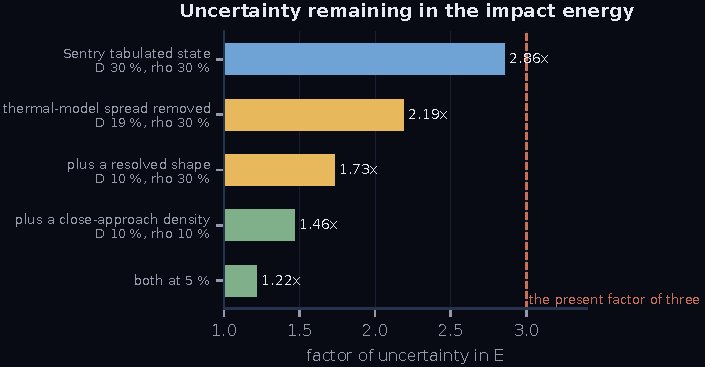
\includegraphics[width=\textwidth]{../figures/fig_energy_ladder.pdf}
\caption{What each link of the energy chain is worth. The present state of
the art leaves a factor of 2.86; removing the thermal-model ambiguity
removes about a quarter of it, and the density term accounts for most of the
remainder.}
\label{fig:energy-ladder}
\end{figure}

\figref{fig:energy-ladder} is the managerial summary of Part II. Each bar is
the factor by which the impact energy remains uncertain once the stated
measurements are in hand. The first bar reproduces the field's own published
statement --- a factor of three --- which is a useful check that the
arithmetic is calibrated against something outside this book.

The decomposition matters more than the total. Removing the thermal-model
ambiguity, by measuring the shape directly, takes the factor from 2.86 to
2.19. Adding a density from a close-approach mass takes it to 1.46. The
remaining gap is the difference between a hazard class that is assigned and
one that is known.

\section{How often this happens}

An energy is only meaningful against a rate of arrival. The European Space
Agency's Near-Earth Object Coordination Centre's background-impact model
gives the frequency \(f_b\) of impacts of a given energy as
\begin{equation}
f_b \approx 0.03\,E^{-0.8}
\quad \mathrm{per\ year},
\label{eq:background}
\end{equation}
with \(E\) in megatons. The model is steeply decreasing, which is the point:
the energies that dominate the casualty risk are the ones that arrive least
often, and they are also the ones the catalogue characterises worst.

\begin{table}[!htbp]
\centering
\small
\caption{Background impact frequency against energy, from the ESA Near-Earth
Object Coordination Centre model.}
\label{tab:background}
\begin{tabularx}{\textwidth}{@{}P{1.16in}P{1.40in}Y@{}}
\toprule
\rowcolor{panel}
\textbf{Energy} & \textbf{Frequency} & \textbf{One impact per} \\
\midrule
\(10^{-3}\) Mt & \(2.4\times 10^{-2}\) a year & 42 years \\
\rowcolor{panel}
\(10^{-2}\) Mt & \(5.9\times 10^{-3}\) a year & 170 years \\
\(10^{-1}\) Mt & \(1.5\times 10^{-3}\) a year & 700 years \\
\rowcolor{panel}
1 Mt & \(3.0\times 10^{-4}\) a year & 3,300 years \\
6.5 Mt & \(8.4\times 10^{-5}\) a year & 12,000 years \\
\rowcolor{panel}
\(10^{2}\) Mt & \(2.5\times 10^{-5}\) a year & 40,000 years \\
\(10^{6}\) Mt & \(7.5\times 10^{-7}\) a year & 1.3 million years \\
\bottomrule
\end{tabularx}
\end{table}

Two observations follow. The first is that the events in the 140-metre class
arrive roughly once in twelve thousand years, which is exactly the timescale
over which the astrometric uncertainty at long horizons has to be defended.
The second is that the probability of any particular object being the one
that hits is small --- but the number of objects that could be the one that
hits is large, and the population of uncharacterised objects is 9,966
objects in the hazard class that have no physical account at all.

\section{The chain, closed and annotated}

\begin{table}[!htbp]
\centering
\small
\caption{The accountability chain, with the measurement that closes each
link and what the link is currently worth.}
\label{tab:accountability-chain}
\begin{tabularx}{\textwidth}{@{}P{1.24in}P{1.32in}Y@{}}
\toprule
\rowcolor{panel}
\textbf{Link} & \textbf{Closed by} & \textbf{Status} \\
\midrule
Shape to volume & resolved imaging & available, at a scale nothing is
currently assigned to \\
\rowcolor{panel}
Volume to mass & bulk density & unresolved; a factor of 2.7 \\
Mass to energy & impact speed & well determined \\
\rowcolor{panel}
Energy to hazard class & the scale's definitions & exact, given the energy \\
\bottomrule
\end{tabularx}
\end{table}

\begin{keytakeaways}
\item A 140-metre object delivers several megatons at typical impact
speeds, and the choice between a rubble pile and a coherent body moves it
across the threshold between local and regional damage.
\item The Level 1 notification threshold is proportional to the inverse of
the energy, so the energy uncertainty moves the notification boundary.
\item Removing the thermal-model ambiguity takes the residual energy factor
from 2.86 to 2.19; adding a close-approach density takes it to 1.46.
\item Background impacts at these energies arrive once in twelve thousand
years, which is the same timescale as the astrometric uncertainty the
community must defend.
\end{keytakeaways}


\part{The Probability Chain}
\label{part:probability}
% =====================================================================
%  Chapter 11 — The \idxw{Keyhole} and How It Is Constructed
% =====================================================================

\chapter{The Keyhole and How It Is Constructed}
\label{ch:keyhole}

The keyhole\idx{Keyhole} is the most efficient idea in planetary defence, and it is also
the one most often misdescribed. It is not a place on the Earth. It is a
narrow window on a plane, and an object passes through it or it does not.
This chapter constructs the window from first principles, because the
construction is what determines how much a physical measurement is worth.

\section{The target plane}

When an asteroid's orbit is propagated to a close encounter with a planet, the
trajectory is described in a plane perpendicular to the planet's approach
direction: the target plane\idx{Target plane}, or B-plane. Two coordinates on that plane locate
the impact parameter: the component along the direction of the planet's
motion, called the along-track coordinate\idx{Along-track coordinate} \(\zeta\), and the component across
it, called the cross-track coordinate \(S\).

The impact parameter\idx{Impact parameter} itself is the distance of the object's centre from the
planet's centre at the encounter epoch,
\begin{equation}
b = \sqrt{S^{2} + \zeta^{2}},
\label{eq:bplane}
\end{equation}
and a collision occurs when \(b\) is smaller than the sum of the two radii.

\begin{deeper}{Why the target plane and not the sky}
Because the planet moves. The distance at which an object passes the Earth
depends on where it is in the sky relative to the Earth's motion at the
moment of passage, not on where it is relative to the stars. An observer on
the Earth's surface, looking at the same object on two different nights, sees
it in the same place in the stars, and the planet's own motion carries the
impact parameter\idx{Impact parameter} around by a very large amount. The target plane\idx{Target plane} removes
that motion and leaves the geometry of the encounter itself.
\end{deeper}

\section{From a collision to a keyhole}

The set of positions on the target plane\idx{Target plane} that produce a collision is a
region of finite width, because the collision is not a point. The width of
that region is set by the sum of the radii and by the geometry of the
approach: at a grazing encounter the effective collision cross-section is
enlarged, and the region is elongated along the direction of the relative
velocity.

The region is called a keyhole\idx{Keyhole}, and its dimensions for a given encounter are
computable from the published encounter geometry. For the 2036 encounter of
Apophis with the Earth, the published keyhole\idx{Keyhole} width is 616.16 metres.

That is a very narrow window, and the narrowness is the entire point. A
keyhole that were a thousand kilometres wide would be a corridor; a keyhole
six hundred metres wide is a target.

\section{The probability, and what it is a function of}

The impact probability is the fraction of the probability distribution of the
along-track coordinate\idx{Along-track coordinate} that falls inside the keyhole. If the along-track
distribution is Gaussian with standard deviation \(\sigma_\zeta\), and the
keyhole is a strip of half-width \(w/2\) centred on \(\zeta_c\), then
\begin{equation}
P = \int_{\zeta_c - w/2}^{\zeta_c + w/2}
\frac{1}{\sigma_\zeta\sqrt{2\pi}}
\exp\!\left(-\frac{\zeta^{2}}{2\sigma_\zeta^{2}}\right)\,\mathrm{d}\zeta.
\label{eq:keyhole-prob}
\end{equation}

Three things follow immediately, and they are worth separating because they
are confused constantly.

The probability is a function of the \emph{width} of the keyhole, which is
fixed by the geometry of the encounter. No amount of characterisation changes
it.

The probability is a function of the \emph{position} of the keyhole relative
to the distribution, which is set by the object's physical properties. This
is the term that a characterisation campaign moves.

The probability is a function of \(\sigma_\zeta\), the width of the
along-track distribution, which is set by the astrometry.

\section{Reconstructing the published number}

The published 2036 impact probability for Apophis is \(7.07\times 10^{-9}\),
the keyhole width is 616.16 metres, and the keyhole centre sits 4.77 sigma
out in the along-track distribution. Those three numbers are not independent,
and the book's own generator reconstructs them from one another.

Take the along-track distribution to be Gaussian with standard deviation
\(\sigma_\zeta\). At a centre position of \(z = -4.77\) standard deviations,
the probability density per unit length is
\begin{equation}
\phi(-4.77) = \frac{1}{\sqrt{2\pi}}\exp\!\left(-\frac{4.77^{2}}{2}\right)
= 4.57\times 10^{-6},
\end{equation}
in units of inverse sigma. The keyhole's full width in units of sigma is
\(616.16/\sigma_\zeta\). The probability is the product, and setting it equal
to the published \(7.07\times 10^{-9}\) and solving gives
\begin{equation}
\sigma_\zeta = 398.5\ \mathrm{km}.
\label{eq:sigmazeta}
\end{equation}

The arithmetic closes: with that value of \(\sigma_\zeta\), the computed
probability is \(7.07\times 10^{-9}\), which is the published number. The
along-track uncertainty on the 2036 encounter is therefore about four
hundred kilometres, and the keyhole is six hundred metres wide --- roughly
one and a half parts in a thousand of the distribution's width, sitting
almost five sigma out in its tail.

\begin{table}[!htbp]
\centering
\small
\caption{What one standard deviation of the along-track distribution is
worth, at the 2036 keyhole.}
\label{tab:tail-sensitivity}
\begin{tabularx}{\textwidth}{@{}P{1.55in}P{1.01in}Y@{}}
\toprule
\rowcolor{panel}
\textbf{Shift of the keyhole centre} & \textbf{Probability factor} &
\textbf{Interpretation} \\
\midrule
0.1 per cent of \(\sigma\) & 1.00 & negligible \\
\rowcolor{panel}
1 per cent of \(\sigma\) & 1.05 & a few kilometres \\
10 per cent of \(\sigma\) & 1.61 & forty kilometres \\
\rowcolor{panel}
100 per cent of \(\sigma\) & 118 & four hundred kilometres \\
\bottomrule
\end{tabularx}
\end{table}

\tabref{tab:tail-sensitivity} is the magnification that the tail provides,
and it is derived from the Gaussian directly: the probability ratio between
two positions \(z_1\) and \(z_2\) in the tail is
\(\exp\left(z_{1}(z_{2}-z_{1})\right)\), and at \(z = 4.77\) the exponent is
large enough that a shift of one standard deviation changes the answer by a
factor of 118.

\section{What this chapter has established}

The keyhole is a narrow window in the tail of the along-track distribution.
Its width is geometric and fixed. Its position is physical, and the physical
assumptions that set its position are the same ones that set the object's
size and density. And because the window sits in the tail, a small change in
the physics is worth a large change in the probability.

The next three chapters work through what that physical position depends
on, and when it matters.

\begin{keytakeaways}
\item The impact probability is the fraction of the along-track distribution
that falls inside a window whose width is fixed by the encounter geometry.
\item The window's position relative to the distribution is physical, and it
is the term a characterisation campaign moves.
\item The published 2036 numbers are mutually consistent: a 616.16-metre
keyhole at 4.77 sigma with an along-track sigma of 398.5 kilometres
reproduces the published probability of \(7.07\times 10^{-9}\) exactly.
\item At that position in the tail, a shift of one standard deviation in the
keyhole centre changes the probability by a factor of 118.
\end{keytakeaways}

% =====================================================================
%  Chapter 12 — The \idxw{Yarkovsky} Drift
% =====================================================================

\chapter{The Yarkovsky Drift}
\label{ch:yarkovsky}

A body that is heated unevenly and cooled unevenly does not receive and
re-emit sunlight symmetrically, and it therefore experiences a small,
persistent thrust. The effect is called Yarkovsky\idx{Yarkovsky} after the scientist who
identified it in the nineteenth century, and it is the reason the orbits of
small asteroids are not closed ellipses.

For a body of this class the effect is not a curiosity. It is the
accumulated along-track displacement that decides whether a keyhole is hit.

\section{The mechanism}

The body's rotation carries surface elements through the day and night
cycle. A surface element that is heated and then cools radiates at
temperatures that depend on when it was last illuminated, and the radiation
leaves preferentially in the direction normal to the surface. The net recoil
over a rotation is a small force along the spin axis and a small torque
about it.

The force depends on the obliquity, on the thermal properties of the surface
and on the spin rate. Writing it in the form used in the 2012 study of
Yarkovsky\idx{Yarkovsky} and YORP,
\begin{equation}
\frac{d a}{d t} \propto
\frac{(1-A)\cos\gamma}{\sqrt{a\,\rho_b\,D}}\,
f(\Theta, \omega),
\label{eq:yarkovsky}
\end{equation}
where \(A\) is the albedo, \(\gamma\) is the angle between the spin axis and
the ecliptic normal, \(\rho_b\) is the bulk density, \(D\) is the diameter and
\(\omega\) the rotation rate.

Three of the five terms are physical properties that a characterisation
campaign measures: the albedo, the bulk density and the diameter. The
fourth, the spin axis, comes from the lightcurve. The fifth, the thermal
parameter \(\Theta\), does not.

\section{The thermal parameter, and why the book will not extrapolate it}

The function \(f(\Theta, \omega)\) contains the thermal parameter\idx{Thermal parameter}
\begin{equation}
\Theta = \frac{\Gamma\,\omega}{\varepsilon\,\sigma\,T_{\mathrm{SSP}}^{3}},
\label{eq:theta}
\end{equation}
where \(\Gamma\) is a shape-and-latitude factor of order unity,
\(\varepsilon\) the emissivity, \(\sigma\) the Stefan-Boltzmann constant and
\(T_{\mathrm{SSP}}\) the temperature of a surface element at the
steady-state temperature of the sub-solar point. For a body with a low
thermal inertia, \(T_{\mathrm{SSP}}\propto D^{-1/2}\), so \(\Theta\) grows
steeply as the body shrinks.

This is the reason the book refuses to extrapolate an absolute drift rate
across the size range between the calibration object and the class of
interest. The scaling laws in \eqref{eq:yarkovsky} isolate the explicit size
and density factor, and that factor can be quoted as a ratio. The thermal
parameter cannot be scaled that way, because it varies with size through a
different and stronger dependence.

\begin{deeper}{The rule, and why it exists}
The 2012 calibration is the asteroid pseudo-Geographos: 2,560 metres in
diameter, a bulk density of 2,500 kilogrammes per cubic metre, a semimajor
axis of 1.246 astronomical units, a Yarkovsky\idx{Yarkovsky} drift of 18.1 metres per year
and a YORP acceleration of \(2.26\times10^{-3}\) radians per year squared.
Applying the scaling laws to a 60-metre body gives ratios of the order of
forty to a hundred for the drift and of several hundred to several thousand
for the torque. Those ratios are the size-and-density part of the effect and
nothing else. The published absolute drift rates for real objects are used
wherever an absolute drift appears in this book, and no absolute drift is
derived by scaling.
\end{deeper}

\begin{table}[!htbp]
\centering
\footnotesize
\caption{The size-and-density part of the scaling laws, expressed as ratios
to the pseudo-Geographos calibration. The thermal-parameter factor is
excluded, and the ratios are therefore lower bounds on the true scaling.}
\label{tab:rg-ratios}
\begin{tabularx}{\textwidth}{@{}P{0.99in}P{0.86in}P{0.86in}Y@{}}
\toprule
\rowcolor{panel}
\textbf{Diameter and density} & \textbf{Yarkovsky} & \textbf{YORP} &
\textbf{Comment} \\
\midrule
51 m, 1,300 & \(\times 96\) & \(\times 4{,}827\) & the YR4 fast-rotating
model with a rubble pile \\
\rowcolor{panel}
51 m, 2,800 & \(\times 45\) & \(\times 2{,}241\) & as above, coherent \\
60.8 m, 1,300 & \(\times 81\) & \(\times 3{,}409\) & the YR4
thermophysical model, rubble pile \\
\rowcolor{panel}
60.8 m, 2,800 & \(\times 38\) & \(\times 1{,}583\) & as above, coherent \\
140 m, 1,300 & \(\times 35\) & \(\times 643\) & the catalogue's threshold
class \\
\rowcolor{panel}
140 m, 2,800 & \(\times 16\) & \(\times 299\) & as above, coherent \\
\bottomrule
\end{tabularx}
\end{table}

The ratios in \tabref{tab:rg-ratios} are large because the calibration object
is two orders of magnitude larger, and \eqref{eq:yarkovsky} makes the
dependence explicit. The practical consequence is that the smaller the body,
the more the drift rate depends on knowing its size and density --- which is
precisely the class where the catalogue knows neither.

\section{What a shape measurement does, and does not, buy here}

This is the point at which an over-statement is easiest to make, and the
published evidence is unusually clear.

The same 2012 study finds that gross shape differences move the Yarkovsky
drift by only about ten per cent for objects of the same size. What enhances
the drift appreciably is \emph{roughness beaming} --- the effect of a rough
surface on the thermal emission --- which can raise it by tens of per cent
and, in the most favourable cases, by a factor of two. And it finds that the
sensitivity to the size is three times the sensitivity to the shape: a three
per cent error in the diameter produces a three per cent error in Yarkovsky,
while the same three per cent in the shape produces only about one per cent
in the drift.

The conclusion is uncomfortable but it is the right one, and the book states
it rather than avoiding it: \textbf{a resolved shape measurement does not
substantially improve the Yarkovsky drift}. It improves the YORP torque,
which Chapter 13 takes up, and it supplies the volume on which the entire
accounting chain rests, and it supplies the spin pole that enters
\eqref{eq:yarkovsky} through \(\cos\gamma\). But the drift itself is
governed by the size, the density and the thermal parameter.

This is why the argument of the book is anchored on the accounting chain and
on the close encounter, and not on the drift. The drift is where the shape
measurement earns its keep through the spin state and the density, and not
through the shape's effect on the thermal emission.

\section{What the live case says}

The 2025 JWST analysis of 2024~YR4 makes the connection explicit in its own
discussion. The object's seasonal heating is negligible for the March 2025
observations, because of the near-equator-on viewing geometry; the seasonal
Yarkovsky drift is expected to dominate the diurnal component and might
become measurable during future encounters; and the non-gravitational forces
such as the Yarkovsky effect contribute to the growing uncertainty in the
future trajectory of the object, making very long-term predictions
impossible.

The wording matters. The drift is not yet measurable for this object. It is
expected to become measurable at a future encounter. Until then it is a
term in a covariance matrix that grows with the arc, and it is one of the
reasons the JWST analysis explicitly declines to offer a long-term impact
probability.

\begin{keytakeaways}
\item The Yarkovsky drift depends on the albedo, the obliquity, the density,
the diameter and a thermal parameter\idx{Thermal parameter} that does not scale with them.
\item The scaling laws give the size-and-density ratios, which for this class
are between sixteen and ninety-six times the calibration object, but the
book does not extrapolate an absolute drift across that range.
\item A resolved shape measurement improves the drift by only about ten per
cent; what it improves materially is YORP, the volume and the pole.
\item For 2024 YR4 the drift is not yet measurable and is expected to become
measurable at a future encounter, and it is already a growing term in the
trajectory uncertainty.
\end{keytakeaways}

% =====================================================================
%  Chapter 13 — The YORP \idxw{Torque}
% =====================================================================

\chapter{The YORP Torque}
\label{ch:yorp}

The YORP effect --- Yarkovsky--O'Keefe--Radzievskii, named for the three
authors whose separate predictions of it turned out to describe the same
phenomenon --- is the torque\idx{Torque} that a rotating body with a non-uniform surface
exerts on itself through the anisotropic re-radiation of sunlight. It is the
mechanism by which a small asteroid's rotation rate changes over decades,
and it is the channel through which a shape measurement does its most
direct work on the probability chain.

\section{The mechanism}

Consider a surface element of a rotating body. It is heated as it rotates
into sunlight and cools as it rotates away. The temperature of that element
therefore varies through the rotation, and the radiation it emits varies with
it. The emitted radiation carries momentum, and the momentum is directed
along the outward normal. Integrating over a surface whose normals are not
uniformly distributed leaves a net torque.

Three properties of the surface determine the result: the distribution of
surface normals, the distribution of roughness, and the obliquity. The
first is what a shape model supplies, and it is why the effect is
shape-sensitive in a way that the Yarkovsky force is not.

The published scaling, from the same 2012 study, is
\begin{equation}
\frac{d\omega}{d t} \propto \frac{1}{\rho_b D^{2}},
\label{eq:yorp}
\end{equation}
with the dependence on the shape and the roughness carried separately. The
diameter enters as the square, and the density linearly.

\begin{table}[!htbp]
\centering
\small
\caption{What the YORP timescale means for the small class. The calibration
object has a torque of \(2.26\times10^{-3}\) radians per year squared.}
\label{tab:yorp-timescale}
\begin{tabularx}{\textwidth}{@{}P{0.91in}P{0.88in}P{0.91in}Y@{}}
\toprule
\rowcolor{panel}
\textbf{Diameter} & \textbf{Density} & \textbf{Torque ratio} &
\textbf{Comment} \\
\midrule
51 m & 1,300 & \(\times 4{,}827\) & the torque\idx{Torque} on this class is
enormous relative to the calibration \\
\rowcolor{panel}
60.8 m & 1,300 & \(\times 3{,}409\) & the YR4 class \\
60.8 m & 2,800 & \(\times 1{,}583\) & as above, coherent \\
\rowcolor{panel}
140 m & 2,800 & \(\times 299\) & the catalogue's threshold class \\
\bottomrule
\end{tabularx}
\end{table}

The ratios in \tabref{tab:yorp-timescale} are the size-and-density part
only, and they are large. A torque\idx{Torque} that would take a 2.5-kilometre object a
decade to spin up would spin a 60-metre object of the same density in a
fraction of a year --- which is physically absurd, and is the reason the
same caveat applies here as in the previous chapter: the full YORP
expression carries a dependence on the shape and on the spin rate that does
not scale with the diameter alone, and the book does not extrapolate an
absolute secular acceleration across two orders of magnitude.

What survives the caveat is the comparative statement, and it is the one
that matters: \textbf{the YORP torque on the small class is enormously larger
relative to its calibration than the Yarkovsky drift is}, by a factor of
roughly fifty in the ratios of \tabref{tab:yorp-timescale} against
\tabref{tab:rg-ratios}. For the small class, the rotation state is a fast
variable, and a fast variable is a variable that a characterisation
campaign has to catch rather than assume.

\section{Why this matters for the book}

Three consequences follow, and they are the reason this chapter exists.

The first is that the spin state is not a slowly varying property that can
be carried forward from a survey lightcurve. For this class it evolves on a
timescale shorter than the gap between observing opportunities. A catalogue
that stores a rotation period measured once is storing a quantity with a
shelf life.

The second is that the shape enters the probability chain directly. The
published sensitivity result is that a three per cent error in the diameter
produces a six per cent error in the YORP torque --- twice the relative
sensitivity of Yarkovsky --- because the torque depends on the shape
directly and the drift does not.

The third is the one that connects this chapter to Chapter 7 and to the
whole architecture. A torque is a vector, and the direction it turns the
body towards depends on where the mass is. The 2022 study of Apophis's
rotation through the 2029 encounter found that the encounter is likely to
change the effective spin rate by up to a factor of two and to shift the
pole by ten degrees or more, and that these changes are very sensitive to
the close-approach attitude and the mass distribution. The spin state is
therefore not merely an input to the torque; it is the \emph{output} of the
encounter, and it is the observable through which the mass distribution
becomes measurable.

\begin{seamnote}{The chain closes in a place nobody expected}
The sequence is: the encounter perturbs the rotation; the change in
rotation is measured from the ground by photometry and a resolved shape; the
change in rotation constrains the mass distribution; the mass distribution
gives the density; the density is the second factor of three in the energy
relation. Every one of these steps is a measurement that a station at the
encounter could support, and the last one is the one the catalogue has never
had.
\end{seamnote}

\section{What a lightcurve alone can and cannot do}

The lightcurve is the workhorse here, and it is worth being precise about
what it delivers and where it stops.

It delivers the rotation period, the direction of the spin pole, and a
low-order shape model, and it does so from a telescope aperture that every
major observatory already owns. It is cheap, it is fast, and it does not
require proximity.

It stops at the resolution of the shape. A lightcurve constrains the
projected outline of the body, and the standard inversion returns the convex
hull of that constraint. The surface normals that the YORP torque depends on
are the normals of the body, not of its convex hull, and the difference is
exactly the concavity that the hull cannot represent.

For a body in this class, with a spin rate that may change by a factor of
two across a close encounter, the shape resolution is the binding limit on
the torque. This is not a limitation of the technique; it is a statement
about what the technique measures. Chapter 17 takes the convex-hull problem
apart in detail, and Chapter 20 works out what an interferometric
measurement of the same body would deliver.

\begin{keytakeaways}
\item YORP depends on the surface normals directly, which is why it is
genuinely shape-sensitive where Yarkovsky is not.
\item The published scaling puts the torque on the small class tens to
hundreds of times the calibration relative to its size and density, and the
book does not extrapolate an absolute secular acceleration across that
range.
\item A three per cent diameter error produces a six per cent YORP error,
twice the relative sensitivity of Yarkovsky.
\item The spin state is the output of a close encounter as well as its input,
and it is the observable through which the mass distribution becomes
measurable.
\end{keytakeaways}

% =====================================================================
%  Chapter 14 — The \idxw{Tail} at 4.77 Sigma
% =====================================================================

\chapter{The Tail at 4.77 Sigma}
\label{ch:tail}

The physical terms and the astrometric terms do not compete on equal
footing, and the reason is not the length of the arc. It is where the
keyhole sits in the distribution. A keyhole at the peak of the along-track\idx{Along-track}
distribution is insensitive to everything; a keyhole four and three-quarter
standard deviations out in the tail\idx{Tail} magnifies every error it is exposed to,
including the errors in the physics.

This chapter puts the two regimes side by side and computes the crossover.

\section{Regime one: a close encounter at seven years}

The 2024~YR4 lunar encounter of 22 December 2032 is the best-documented
near-term case, and the NASA review of the 2024~YR4 episode reports the
\idxw{B-plane} uncertainty for it with unusual clarity. The uncertainty was 270,000
kilometres, and the review records that a single point observation --- from
the Lucy spacecraft had it been available --- could have reduced it to
25,000 kilometres or less. The same review notes that the Lucy team's own
preliminary analysis did not regard this as certain, and that ground-based
observatories would be likely to achieve the same reduction by the end of the
apparition without Lucy.

That last clause is the important one. It means that the astrometric
uncertainty in a close-approach encounter is \emph{cheap} to reduce, and
that the community reduces it routinely.

Now put the physical term on the other side of the ledger. Over the seven
years from 2025 to 2032, an error in the Yarkovsky drift rate produces an
along-track\idx{Along-track} displacement of the object. The book's generator computes it
directly from the published drift-rate error, for a range of assumed drift
rates at a semimajor axis of 1.1 astronomical units.

\begin{table}[!htbp]
\centering
\small
\caption{Along-track displacement over seven years from an error in the
Yarkovsky drift rate, against the astrometric floor for the 2032 encounter.}
\label{tab:along-track}
\begin{tabularx}{\textwidth}{@{}P{1.07in}P{0.82in}P{0.82in}Y@{}}
\toprule
\rowcolor{panel}
\textbf{Drift rate} & \textbf{10 per cent} & \textbf{30 per cent} &
\textbf{Comment} \\
\midrule
50 m/yr & 0.3 km & 0.9 km & a slow drift \\
\rowcolor{panel}
100 m/yr & 0.6 km & 1.7 km & \\
300 m/yr & 1.7 km & 5.1 km & \\
\rowcolor{panel}
1,000 m/yr & 5.7 km & 17.2 km & the fastest case tabulated \\
\midrule
Astrometric floor & 25,000 km & 25,000 km & after a single observation \\
\bottomrule
\end{tabularx}
\end{table}

The comparison in \tabref{tab:along-track} is decisive at this horizon. Even
in the fastest case tabulated, a thirty per cent error in the drift rate
moves the object by 17.2 kilometres over seven years, against an astrometric
uncertainty of 25,000 kilometres after a single extra observation. The
astrometric term dominates by more than three orders of magnitude.

\begin{figure}[!htbp]
\centering
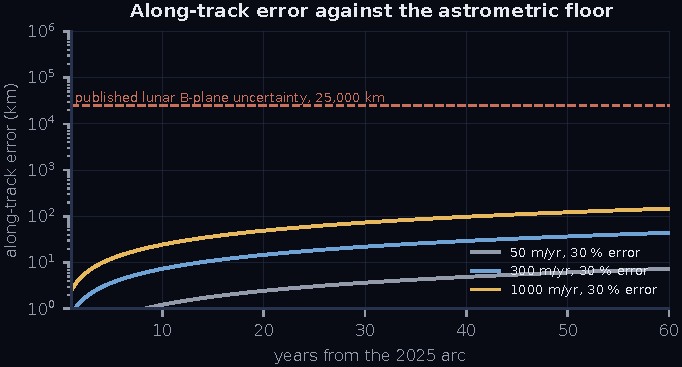
\includegraphics[width=\textwidth]{../figures/fig_along_track.pdf}
\caption{Along-track error against the length of the arc, for three assumed
drift rates and a thirty per cent rate error, against the published
astrometric floor of 25,000 kilometres. The two lines cross nowhere on this
axis: the astrometric term dominates at every horizon the 2032 encounter
reaches.}
\label{fig:along-track}
\end{figure}

The conclusion for this horizon is not that characterisation is useless. It
is that characterisation \emph{does not shorten this particular clock}. A
lunar station would not have made the 2032 lunar encounter probability
better, because the number that dominates that probability is the astrometric
uncertainty, and the astrometric uncertainty is cheap to reduce. That is a
statement about the seven-year horizon, and it is the reason the book's
selection rule declines the lunar platform for short-horizon objects.

\section{Regime two: a keyhole in the tail}

The 2036 encounter of Apophis is the other regime, and the difference is not
the horizon. It is the position of the keyhole.

The along-track\idx{Along-track} distribution for the 2036 encounter has a standard deviation
of 398.5 kilometres, as Chapter 11 reconstructed from the published keyhole
width and probability. The keyhole centre sits 4.77 standard deviations out
in the tail. In that regime the published sensitivity table's factors
translate into along-track displacements, because a probability ratio \(F\) in
the tail\idx{Tail} corresponds to a shift of \(\ln(F)/4.77\) standard deviations.

\begin{table}[!htbp]
\centering
\small
\caption{The published 2036 sensitivities, expressed as along-track
displacements against the 398.5-kilometre astrometric standard deviation.}
\label{tab:magnification}
\begin{tabularx}{\textwidth}{@{}P{1.22in}P{0.66in}P{0.83in}Y@{}}
\toprule
\rowcolor{panel}
\textbf{Varied assumption} & \textbf{Probability} & \textbf{Displacement} &
\textbf{Against the astrometric sigma} \\
\midrule
Diameter 270 \(\pm\) 60 m & \(\times 433\) & 507 km & 1.27 sigma \\
\rowcolor{panel}
Density variance, \(\sigma_\rho^{2} = 0.6\) & \(\times 93\) & 379 km &
0.95 sigma \\
\(\mu_{d0} = 400\) & \(\times 2.25\) & 68 km & 0.17 sigma \\
\rowcolor{panel}
Astrometric standard deviation & --- & 399 km & 1.00 sigma \\
\bottomrule
\end{tabularx}
\end{table}

\tabref{tab:magnification} is the heart of the book's argument about
platform selection. The diameter assumption and the density assumption each
move the 2036 keyhole centre by about one astrometric standard deviation.
They are \emph{not} smaller terms. They are the same size as the astrometric
uncertainty, and they point in a different direction.

\begin{seamnote}{The asymmetry that decides the rule}
Additional astrometry reduces the astrometric standard deviation, and it
reduces it monotonically: more observations, a longer arc, a better
reduction. Additional astrometry does nothing whatever to the 507 kilometres
of displacement contributed by the diameter assumption, or the 379
kilometres contributed by the density, because those are not astrometric
quantities. A rule that selects a platform on the basis of the astrometric
term alone will always choose the ground. A rule that includes the physical
term does not.
\end{seamnote}

\section{The crossover, stated as a principle}

The two regimes are not separated by the horizon and they are not separated
by the instrument. They are separated by whether the keyhole lies in the
tail\idx{Tail} of the along-track distribution.

Where the keyhole is near the peak, the probability is set by the
astrometric uncertainty, the astrometric uncertainty is cheap to reduce, and
characterisation buys nothing. This is the 2032 lunar encounter of
2024~YR4, where a thirty per cent drift-rate error is worth 17 kilometres
against an astrometric floor of 25,000.

Where the keyhole lies several sigma out, the physical terms are of the same
order as the astrometric term and they do not shrink with observing time.
This is the 2036 encounter of Apophis, where the diameter assumption alone is
worth 507 kilometres of displacement.

\begin{table}[!htbp]
\centering
\small
\caption{The two regimes, and what each one implies for a platform.}
\label{tab:regimes}
\begin{tabularx}{\textwidth}{@{}P{1.28in}P{1.28in}Y@{}}
\toprule
\rowcolor{panel}
\textbf{Regime} & \textbf{Dominated by} & \textbf{Implication} \\
\midrule
Keyhole near the peak & astrometry & observe more; the ground does this
best \\
\rowcolor{panel}
Keyhole several sigma out & physics, comparably & measure the size and the
density \\
\bottomrule
\end{tabularx}
\end{table}

This is why the platform-selection rule in Chapter 30 has a conditional
clause at its centre, and why the lunar platform is proposed for a class of
targets rather than for a class of instruments. The lunar station does not
help with the astrometric term. It helps with the physical term. It is worth
exactly as much as the physical term is worth, and the physical term is
worth a great deal when the keyhole is in the tail.

\begin{keytakeaways}
\item At the 2032 lunar encounter of 2024 YR4, a thirty per cent drift-rate
error is worth 17.2 kilometres against an astrometric floor of 25,000 after
a single observation, and the astrometric term dominates by three orders of
magnitude.
\item At the 2036 encounter of Apophis, the diameter assumption alone is
worth 507 kilometres of keyhole displacement and the density assumption 379
kilometres, against an astrometric standard deviation of 399 kilometres.
\item The two regimes are separated by the position of the keyhole in the
tail, not by the length of the arc.
\item More astrometry shrinks the astrometric term and does nothing to the
physical one, which is the asymmetry the selection rule turns on.
\end{keytakeaways}

% =====================================================================
%  Chapter 15 — Why More Data Can Make the Answer Worse
% =====================================================================

\chapter{Why More Data Can Make the Answer Worse}
\label{ch:more-data}

There is a feature of impact monitoring\idx{Monitoring} that unsettles people who meet it
for the first time, and it is worth naming plainly because it undermines the
simplest possible story about how the discipline works. A better orbit can
produce a \emph{higher} impact probability. A more accurate measurement can
make an object look more dangerous than it did before. And a careful
characterisation campaign can move an object \emph{out} of a keyhole and
leave the probability higher than it started.

None of this is a malfunction. All of it follows from the fact that the
impact probability is a conditional probability, and conditions renormalise.

\section{Where the probability actually comes from}

The impact probability is not a property of the object. It is a property of
the object \emph{given the observations}, and it is computed by propagating
the observation-conditioned distribution of the object's position to the
encounter epoch and asking what fraction of that distribution collides.

Two consequences follow immediately.

The first is that the probability is always conditional on something. It is
conditional on the orbital solution, on the arc, on the data reduction, on
the physical parameters. When any of those changes, the probability changes,
and it changes in whichever direction the new information points --- which
may be upward.

The second is that the probability is a density ratio, and a density ratio
moves when the denominator moves. If a refinement of the orbit removes
probability mass from the region that would have collided, the total
probability mass has to go somewhere, and the probability of collision rises.

\begin{seamnote}{The regression that alarms people}
The 2024~YR4 episode is a live instance of the general phenomenon, and the
NASA review of it describes the sequence of revisions to the object's
Earth-impact probability as the orbit was refined. The revisions did not
monotonically decrease the number. This is expected behaviour, and an
organisation that treats a rising number as a failure will make exactly the
wrong decisions.
\end{seamnote}

\section{Why more astrometry cannot fix a physical error}

There is a structural asymmetry here, and it is the reason the previous
chapter's arithmetic has the force it does.

The astrometric uncertainty enters the probability through \(\sigma_\zeta\),
the width of the along-track distribution. More astrometry --- more
observations, a longer arc, a better weighted solution --- reduces
\(\sigma_\zeta\), and the keyhole's probability falls as the distribution
narrows around a fixed keyhole position. The mechanism is well behaved and
monotone, and it is the reason the community's answer to a tail keyhole is
always ``observe more''.

The physical uncertainty enters the probability through the keyhole's
\emph{position}. A better measurement of the diameter or the density changes
where the object will be at the encounter epoch, and therefore changes
whether the keyhole lands on it. This mechanism is not monotone in either
direction. It can move the object into the keyhole or out of it.

The consequence for a programme is uncomfortable but plain. \textbf{There is
no quantity of astrometry that removes a physical error from an impact
probability.} The astrometric term can be driven towards zero; the physical
term can only be driven towards zero by measuring the physics.

\begin{table}[!htbp]
\centering
\small
\caption{The two terms, and what reduces each of them.}
\label{tab:terms}
\begin{tabularx}{\textwidth}{@{}P{1.28in}P{1.28in}Y@{}}
\toprule
\rowcolor{panel}
\textbf{Term} & \textbf{Reduced by} & \textbf{Behaviour} \\
\midrule
Astrometric & more observations, longer arc & monotone; the probability
falls \\
\rowcolor{panel}
Physical & measuring the size, the density, the spin state & not monotone; the
probability may rise or fall \\
\bottomrule
\end{tabularx}
\end{table}

\section{The three forms of the paradox}

The first is the refinement regression: a better orbit raises the
probability because the previous probability was an artefact of the
conditioning. The community's response is correct --- keep observing --- and
the number falls again once the solution is better still.

The second is the physical update: a measurement of the object's diameter or
density moves the keyhole centre and the probability moves with it, in
whichever direction. Here the community's response must be the opposite of
the first. Observing more will not help, because the error is not
astrometric. Measuring the physics is the only route, and it is the route
that is not funded.

The third is the keyhole exit. An object whose probability is high because it
sits in a keyhole has its probability \emph{fall} when the keyhole's centre
is refined away from it, and the fall can be dramatic, because the tail
magnifies the displacement in both directions. This is the good outcome, and
it can look like a mistake in the reporting.

\begin{table}[!htbp]
\centering
\small
\caption{The three behaviours, and what each one calls for.}
\label{tab:paradoxes}
\begin{tabularx}{\textwidth}{@{}P{1.32in}P{1.24in}Y@{}}
\toprule
\rowcolor{panel}
\textbf{Form} & \textbf{What it looks like} & \textbf{What is actually
required} \\
\midrule
Refinement regression\idx{Regression} & the probability rises as the orbit improves &
keep observing; this is the astrometric term \\
\rowcolor{panel}
Physical update & the probability moves when the size or density is
measured & measure more physics; observing will not help \\
Keyhole exit & the probability falls sharply as the centre is refined &
nothing further, but do not treat it as an error \\
\bottomrule
\end{tabularx}
\end{table}

\section{Why this is the argument for characterisation rather than for monitoring}

The monitoring\idx{Monitoring} machinery of the planetary-defence establishment is built on
the first and third of these behaviours and is good at them. It is not
built for the second, because the second requires an instrument, a target
list and an alert path, and none of the three exists in the shape the
situation needs. The documented position, from the 2025 NASA review of the
2024~YR4 episode, is that no automated system currently alerts physical
characterisation sites.

So the paradox is not only a scientific curiosity. It is the mechanism by
which the gap in Part I becomes dangerous rather than merely untidy. A
catalogue that contains 11,725 catalogued objects in the hazard class and
about 9,966 of them without any physical account contains, in statistical
form, 9,966 objects whose keyhole position is unknown. When one of those
objects turns out to be on a trajectory that passes near the Earth, the
monitoring\idx{Monitoring} machinery will do what it does: it will observe, refine, and
renormalise. And the probability it reports will depend on physical
assumptions that nobody has measured.

\begin{keytakeaways}
\item The impact probability is conditional, and a conditional probability
renormalises, so a better orbit can produce a higher probability.
\item The astrometric term is monotone and cheap to reduce; the physical
term is not monotone and no quantity of astrometry reduces it.
\item A physical update that raises the probability is not a malfunction,
and it is the case in which observing more is the wrong response.
\item Nine thousand nine hundred and sixty-six objects in the hazard class
carry an unknown keyhole position, and the machinery to measure it does not
exist.
\end{keytakeaways}


\part{Measuring Shape}
\label{part:shape}
% =====================================================================
%  Chapter 16 — Generalised Projections and the \idxw{Uniqueness} Theorems
% =====================================================================

\chapter{Generalised Projections and the Uniqueness Theorems}
\label{ch:projections}

Every shape measurement in this book is a projection. A photograph of a
rotating body is the body's silhouette against the sky, taken along a
direction that changes as the body turns. A radar image is a projection\idx{Projection} of a
different kind, reconstructed from the delay and the Doppler shift of an
echo. An interferometric image is a projection\idx{Projection} reconstructed from the
visibility and the phase of a fringe pattern.

This chapter asks the question that underlies all of them: what can be
determined from a projection\idx{Projection}, and how many of them are needed?

\section{What a single projection gives}

A projection along a fixed direction of a convex body\idx{Convex body} gives the outline of
its shadow: a convex region whose area is the body's projected area and
whose shape is the body's projected shape. From that one outline, three
things follow immediately --- the projected area, the projected extent in
two orthogonal directions, and the rotation phase at which the projection
was taken.

Three things do not follow, and the list is worth keeping in view because it
is the whole of Chapter 8's argument:

The volume does not follow. A sphere and a flat disk of the same projected
area have the same silhouette and volumes differing by a factor of three.
The projected area constrains the volume only to within the range that the
convex hull of the silhouette allows.

The three-dimensional shape does not follow. A body of revolution\idx{Body of revolution} and an
ellipsoid with the same silhouette are indistinguishable in a single
projection, and so are a thousand non-convex bodies whose shadow agrees.

The orientation of the body in space does not follow, beyond the two
projected axes. The direction of the spin pole is what fixes it, and a
single projection does not fix the pole.

\section{Why the classical uniqueness results matter}

The theory of reconstructing a body from its projections is old and precise,
and three of its results are directly relevant.

A convex body\idx{Convex body} is uniquely determined by the set of all its orthogonal
projections. This is the strongest statement and the least useful, since it
requires infinitely many.

A body of revolution\idx{Body of revolution} is determined by a single projection along its axis of
symmetry. This is the strongest useful statement, and it is why the
rotation state of an asteroid is such valuable information: a body that is
close to a body of revolution\idx{Body of revolution} can be characterised from one projection, and
the residual error is a measure of how far from a body of revolution it is.

And a general body requires a family of projections. For a convex body\idx{Convex body}, the
projections onto a small number of suitably chosen directions --- in the
limit, three generic directions for a polytope --- can determine it, but
``suitably chosen'' is a real constraint: the directions must not share a
degenerate relationship, and a single direction never suffices.

\section{What the rotation supplies}

This is where the astrophysical case differs from the geometric one, and the
difference is favourable in a way that is not obvious before it is stated.

A body on the ground is observed from essentially one direction, and that
direction is fixed by where the observer is. As the body rotates, the
\emph{body's} orientation changes but the \emph{projection direction} does
not. What changes is the shape of the projected outline, because the body
presents different parts of itself to the observer.

That is the whole content of the lightcurve. The brightness of a rotating
body varies because the projected outline and the projected brightness
distribution vary. The variation has a period, and the period is the
rotation period.

So the body does supply a family of projections --- the set of all its
projections over a full rotation. For a body whose projection changes
sufficiently with phase, the set of projections over one rotation carries
the information of a band of directions, and it is that band, rather than a
single outline, that the inversion uses.

\begin{deeper}{Why the inversion is nevertheless not unique}
The band is not the whole sphere of directions. The projections obtained
over one rotation all share the same viewing direction and differ only in
the body's orientation about one axis, so the reconstruction is a body of
revolution about that axis --- up to the non-convexity, which the
projections at different phases can partly expose. The practical result is
the familiar one: a single lightcurve admits a family of shapes and a
family of pole directions, and the standard inversion returns the convex
hull of that family. Additional lightcurves at different apparitions, or a
single resolved image that fixes the geometry directly, are what break the
degeneracy.
\end{deeper}

\section{What this implies for the measurement hierarchy}

The hierarchy of methods in the field follows from this, and it explains why
the cheapest methods produce the least certain results.

\begin{table}[!htbp]
\centering
\small
\caption{What each measurement family determines, and the assumption each
one carries.}
\label{tab:hierarchy}
\begin{tabularx}{\textwidth}{@{}P{1.24in}P{1.32in}Y@{}}
\toprule
\rowcolor{panel}
\textbf{Method} & \textbf{Determines} & \textbf{Carries} \\
\midrule
Lightcurve & period, pole, low-order shape & convexity; the band of
projections is not the whole sphere \\
\rowcolor{panel}
Disk image & the projected outline at one epoch & the shape of that
outline; the volume still needs a model \\
Radar image & the three-dimensional shape directly & the geometry of the
measurement \\
\rowcolor{panel}
Interferometric image & the projected outline at high angular resolution &
the visibility model, and the matching of the baseline to the target \\
\bottomrule
\end{tabularx}
\end{table}

The last row is where the book's argument goes next. An interferometric
image is, in principle, the best of the four, because the angular resolution
it delivers is a function of the baseline rather than of the target's
distance, and because the resolution can be set by choosing the baseline
rather than by waiting for a close approach.

The catch is that an interferometer does not produce a picture by itself. It
produces a visibility and a phase, and the picture is reconstructed from
those, and the reconstruction has an assumption attached: a model of what
the body's brightness distribution looks like on the sky. That model is the
subject of Chapter 20.

\begin{keytakeaways}
\item A single projection determines the projected area and the projected
extent, and does not determine the volume, the three-dimensional shape or
the orientation.
\item The rotation supplies a band of projections rather than a single one,
which is why a lightcurve carries more information than a single image ---
and why it still returns a convex hull.
\item The classical uniqueness\idx{Uniqueness} results set the target: a body of revolution
is determined by one axial projection, and a general convex body needs a
family.
\item An interferometer's resolution is set by the baseline rather than by
the distance, which is why it is the only method that can image a small
object without waiting for a close approach.
\end{keytakeaways}

% =====================================================================
%  Chapter 17 — Lightcurve Inversion\idx{Lightcurve inversion} and the Convex Hull
% =====================================================================

\chapter{Lightcurve Inversion and the Convex Hull}
\label{ch:lightcurve}

The lightcurve inversion\idx{Lightcurve inversion} is the workhorse of asteroid characterisation. It
has produced more shape models than every other method combined, it uses
telescopes that already exist, and it returns a coherent three-dimensional
body with a spin axis and a rotation period. This chapter asks what it
returns and what the answer costs.

\section{What the inversion does}

The procedure is standard and worth stating in full, because the place the
assumption enters is usually a single sentence that is easy to miss.

A set of photometric observations of a rotating body is recorded. A model is
constructed: a shape, an orientation and a rotation rate, such that the
model's predicted brightness variation as it rotates matches the observed
variation. The model parameters are then searched for the best fit.

The fitted parameters are the rotation period, the direction of the spin
pole, and the shape. The shape that comes out of the standard inversion is
the \emph{convex hull} of the body consistent with the observations ---
because the constraint set is not convex and the hull is the standard way to
report a single answer from it.

The assumption is not a modelling convenience. It is the statement that the
body is convex, and it is made silently, because a convex body is the
simplest consistent answer and because the database that holds these models
records it.

\section{What the record contains}

The scale of the effort is remarkable and it is the reason the method
dominates the field. The asteroid models database\idx{Asteroid models database} reached roughly 25,000
models by October 2026, a figure that tripled the catalogue in five years.
The sample underlying the most recent analysis covered 881 near-Earth
asteroids, of which 47 received a model.

The throughput comparison that comes with it is the most useful summary of
the field's measurement history there is. Taken across the epochs of the
field's major reviews, the number of resolved shape models produced by each
method has moved as follows:

\begin{table}[!htbp]
\centering
\small
\caption{Resolved shape models by method, across the epochs of the field's
major reviews. The figures are the accumulated totals.}
\label{tab:throughput}
\begin{tabularx}{\textwidth}{@{}P{1.15in}P{0.78in}P{0.78in}Y@{}}
\toprule
\rowcolor{panel}
\textbf{Method} & \textbf{Earliest} & \textbf{Latest} & \textbf{Comment} \\
\midrule
Interferometry & 5 & \(10^{2}\) & the only resolved method with a
projected hundred \\
\rowcolor{panel}
Photometry & 30 & \(10^{4}\) & the workhorse; lightcurve inversions \\
Fly-by & 6 & fewer than 15 & one per spacecraft encounter \\
\bottomrule
\end{tabularx}
\end{table}

\tabref{tab:throughput} contains the argument of this book in one line.
Interferometry, the only method that produces a resolved shape without
requiring proximity, is the lowest-yield resolved method in the field, and
the field's own roadmap projects a hundred of them. The ten thousand
photometric inversions are low-order convex bodies. The fewer than fifteen
fly-by images are the only true three-dimensional shapes in existence.

\section{The cost of the convexity, and the evidence for it}

The question the convex-hull assumption raises is quantitative: how wrong is
a convex hull, for a real small body?

The best available evidence is the one measurement that bypassed the
question, and it is the 2017 radio occultation of (372) Palma discussed in
Chapter 8. The silhouette it measured was slightly elongated and had a
concave edge, and the roundness\idx{Roundness} parameter --- the ratio of the inscribed to
the circumscribed circle --- had a mean of 0.866 with a standard deviation of
0.093 over the fitted shape ensemble, giving a departure from a perfect
circle of ten to twenty per cent.

Twenty per cent is not a small number, and it is worth being precise about
what it does and does not imply. The roundness\idx{Roundness} parameter is a two-dimensional
measure of the silhouette. It is not the volume error. A body that is
slightly elongated in projection may be considerably less voluminous than
its convex hull if it is also concave, and considerably more voluminous than
its projection if it is oblate in the third dimension. The honest statement
is a bound and a direction: \textbf{real small bodies depart from the
convex ideal by tens of per cent in their silhouettes, so convex-hull volumes
carry systematic errors of that order, and the errors are one-sided --- the
hull is always at least as large as the body.}

\begin{seamnote}{Why the one-sidedness is good news}
Because the convex hull always overstates the volume, and therefore
overstates the mass at a fixed density, a lightcurve inversion\idx{Lightcurve inversion} tends to
overstate the energy. That is a conservative error in the direction of
concern. It is also an error that nobody has bounded, because the field does
not have the resolved silhouettes of small bodies against which to bound it.
A single measurement that would bound it exists, and it is the measurement
the rest of this book is about.
\end{seamnote}

\section{The second limitation, which is not about shape}

The convex hull is the assumption that gets discussed. The limitation that
gets less attention is that a lightcurve inversion returns a shape, and a
shape is not a size.

The diameter that goes into the energy chain is not the diameter of the
shape model. It is the diameter consistent with the model's projected area
and the object's absolute magnitude --- which is a photometric inversion with
its own assumptions, and which carries the albedo into the answer. The
lightcurve inversion therefore delivers a shape, and then a separate step
turns the shape into a diameter, and that step is where the albedo
degeneracy re-enters.

A resolved image does not have this problem in the same way, because the
projected area is measured directly and the albedo is an output rather than
an input. That difference is the entire content of the argument in
\tabref{tab:routes}.

\section{What the method is good for}

It is worth ending this chapter by saying plainly what the lightcurve
inversion is good for, because the chapter is not a criticism of it.

It is good for the spin state. The period and the pole are its strongest
products, they are obtained from telescopes that exist, and they are needed
by everything downstream. The pole enters the Yarkovsky drift through
\(\cos\gamma\); the period enters the YORP torque and the lightcurve
amplitude that goes with it.

It is good for identifying the objects worth looking at. A lightcurve is
cheap and it is fast, and an object whose lightcurve shows a large amplitude
and a short period is an object whose shape matters.

It is good for finding the objects that a close approach will change. The
spin state is the observable through which a close encounter reveals the
mass distribution, and the lightcurve is how the spin state is measured.

What it is not good for is the volume. And the volume is what the energy
chain is built from.

\begin{keytakeaways}
\item The standard lightcurve inversion returns the convex hull of the
consistent set, so the convexity assumption is made silently.
\item The field has produced roughly 25,000 photometric models against fewer
than fifteen fly-by shapes and a projected hundred interferometric ones.
\item The Palma silhouette shows real bodies departing from the convex ideal
by tens of per cent, and the hull error is always one-sided.
\item The lightcurve's strongest products are the period and the pole, and
its weakest is the volume, which is the quantity the energy chain needs.
\end{keytakeaways}

% =====================================================================
%  Chapter 18 — \idxw{Radar} Range-Doppler and the Fourth-Power Wall
% =====================================================================

\chapter{Radar Range-Doppler and the Fourth-Power Wall}
\label{ch:radar}

Radar\idx{Radar} is the method that answers the question this book is about most
completely. It gives the three-dimensional shape, the rotation state and the
mass, in one measurement, from a non-cooperative target, with no assumption
about convexity and none about the body's thermal behaviour. It is also the
method with the hardest physical limit in the field, and understanding that
limit is what tells you where the complementary capability has to sit.

\section{What radar measures}

A radar\idx{Radar} pulse is transmitted towards the target and its echo is received.
Three properties of the echo carry information.

The \emph{delay} between transmission and reception gives the range to the
target, and the range to each scattering element gives the depth structure.

The \emph{Doppler shift} of the echo gives the line-of-sight velocity of
each scattering element, and the velocity field gives the rotation.

The \emph{amplitude} of the echo gives the radar\idx{Radar} cross-section\idx{Radar cross-section}, which
depends on the size of the scattering elements and, in the polarimetric
case, on their shape and on the roughness of the surface. The polarimetric
signature is what distinguishes a consolidated surface from a particulate
one, and it is therefore a direct diagnostic of the density question that
Chapter 7 identified.

The combination of range and Doppler is what produces the image: the classic
delay-Doppler\idx{Delay-Doppler} inversion reconstructs a three-dimensional shape from a
two-dimensional data set, and it does so without assuming anything about the
body's convexity.

\begin{table}[!htbp]
\centering
\small
\caption{What the radar techniques deliver, and their limits.}
\label{tab:radar-methods}
\begin{tabularx}{\textwidth}{@{}P{1.24in}P{1.32in}Y@{}}
\toprule
\rowcolor{panel}
\textbf{Technique} & \textbf{Delivers} & \textbf{Constraint} \\
\midrule
Single-dish radar & range, Doppler, and a radar cross-section\idx{Radar cross-section} & needs a
radar-crossing object and a large dish \\
\rowcolor{panel}
\idxw{Bistatic radar} & range, Doppler, and a delay-Doppler\idx{Delay-Doppler} image & needs a second
station and a common view \\
\idxw{Delay-Doppler} imaging & the three-dimensional shape & the reconstruction is
ill-conditioned at low signal \\
\rowcolor{panel}
Polarimetry & the surface state, and hence a density diagnostic & the
weakest signal of the four \\
\bottomrule
\end{tabularx}
\end{table}

\section{The fourth-power wall}

The reason radar cannot characterise the catalogue is a power law, and the
exponent is what matters.

The flux of a body falls as the inverse square of its distance, so the
power it intercepts and scatters falls as \(R^{-2}\). The echo is then
spread over a solid angle that grows as \(R^{2}\), so the received power per
unit solid angle falls as \(R^{-4}\).

\begin{equation}
P_{\mathrm{recv}} \propto \frac{\sigma}{R^{4}},
\label{eq:radar4}
\end{equation}
with \(\sigma\) the radar cross-section. The fourth power is brutal. Doubling
the range divides the received power by sixteen. A radar cross-section\idx{Radar cross-section} that
is adequate at a tenth of an astronomical unit is 10,000 times weaker at
one astronomical unit.

This is the wall that shapes the whole field. More than 1,100 near-Earth
objects have been observed by radar at some point, and a few dozen have
complete radar shape models. The difference between those two numbers is the
combination of the fourth-power law\idx{Fourth-power law}, the need for a radar-crossing object,
and the reality that the dishes are on the Earth and the targets are not.

\begin{figure}[!htbp]
\centering
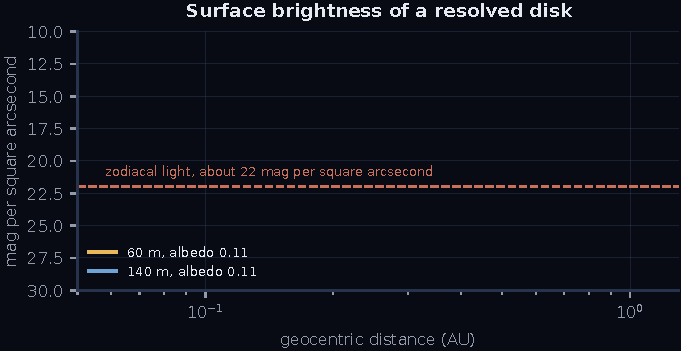
\includegraphics[width=\textwidth]{../figures/fig_brightness.pdf}
\caption{The surface brightness of a resolved disk of the 60-metre and
140-metre classes against distance, against the zodiacal background at about
22 magnitudes per square arcsecond. The lunar sky is not the constraint on
the optical channel: the target is 18 to 22 magnitudes above the
background.}
\label{fig:brightness}
\end{figure}

\section{Why the Moon does not help the radar problem, and does help the optical one}

This is where the owner's original instinct --- a ranging beam from the Moon
--- has to be handled carefully, because the instinct is right about the
physics and wrong about the comparison.

A radar system on the Moon would have a range advantage over a ground
system, and the fourth-power law\idx{Fourth-power law} means that a range advantage is worth a
great deal. But the advantage is modest in the regime that matters: for a
target at 1.3 astronomical units, the Moon's range advantage over the Earth
is only about 1.3 in the geometric sense, and the fourth-power law\idx{Fourth-power law} turns a
factor of 1.3 in range into a factor of about 2.9 in received power. That is
not nothing, but it is not the difference between characterising the
catalogue and characterising a handful of objects.

The reason is structural, and it is the reason the book puts the optical
channel rather than the radar channel at the centre of the lunar case. The
optical channel's range dependence is the inverse square of the flux law,
which is far milder, and the optical channel does not require the target to
be radar-crossing, which is a severe selection effect: only a few per cent
of small near-Earth objects have surfaces that are radar-bright enough to
detect at all.

\begin{table}[!htbp]
\centering
\small
\caption{The two channels compared, on the physics rather than on the
instruments.}
\label{tab:channels}
\begin{tabularx}{\textwidth}{@{}P{1.19in}P{1.37in}Y@{}}
\toprule
\rowcolor{panel}
\textbf{Property} & \textbf{Optical} & \textbf{Radar} \\
\midrule
Range dependence & \(R^{-2}\) on the flux & \(R^{-4}\) on the echo \\
\rowcolor{panel}
Target selection & any object bright enough & only radar-crossing objects \\
Shape & a projection, needs a model & three-dimensional, direct \\
\rowcolor{panel}
Mass & not directly & yes, from the trajectory \\
Density & no & yes, from polarimetry \\
\bottomrule
\end{tabularx}
\end{table}

The last two rows are the reason radar remains indispensable and the reason
it cannot be the answer to the catalogue: it is the only method that gives
the mass and the density, and it is the method whose reach is limited to a
small fraction of the population.

\section{Bistatic radar, and the Moon as a reflector}

Bistatic radar\idx{Bistatic radar} separates the transmitter from the receiver, and that
separation buys two things: a much larger effective baseline, and the
ability to use a body that is not a radio telescope as the transmitter or the
reflector.

The Australian record is the strongest demonstration in the field. Using the
Green Bank Telescope and the Parkes observatory as a bistatic pair, more than
fifty near-Earth objects have been characterised since 2015, including
delay-Doppler\idx{Delay-Doppler} images and polarimetric measurements.

The Moon is itself a bistatic radar\idx{Bistatic radar} reflector of a kind, and the concept has
been demonstrated: radio-occultation work has used the Moon's limb as a
diffracting edge, and the 2017 occultation of (372) Palma measured by the
Very Long Baseline Array is the most precise use of a lunar limb as an
optical element in the history of the field.

\begin{seamnote}{The pattern, and the book's use of it}
Every one of these lunar exploits uses the Moon as a passive reflector or a
diffracting edge. None of them uses the Moon as a telescope. The book follows
the same pattern: the lunar contribution is a stable baseline and a long
observing window, and the instrument that uses them is an optical
interferometer, because that is the instrument for which a kilometre-scale
stable baseline changes the answer.
\end{seamnote}

\begin{keytakeaways}
\item Radar delivers the three-dimensional shape, the spin state and the mass,
and it is the only method that answers the density question directly.
\item The received echo power falls as the fourth power of range, and that
law is the wall the field has never got past.
\item The lunar range advantage is worth about a factor of three in received
power at 1.3 astronomical units, which is real but not transformative, and
the radar selection effect is the harder constraint.
\item The lunar exploits that have worked are all passive: the Moon as a
diffracting edge and as a bistatic reflector, never as a telescope.
\end{keytakeaways}

% =====================================================================
%  Chapter 19 — Disk-Resolved Imaging and the Close-Approach Window
% =====================================================================

\chapter{Disk-Resolved Imaging and the Close-Approach Window}
\label{ch:disk-imaging}

There are two ways to see an asteroid as a disk rather than as a point. One
is to be near it. The other is to have an aperture large enough, or a
baseline long enough, that its angular size is resolved from far away. The
first is the method that has actually produced images; the second is the
method this book is proposing. This chapter is about the first, and about
what it costs.

\section{What a resolved disk gives}

A resolved image of a rotating body is worth more than a lightcurve, and the
reason is geometric. A lightcurve gives the body's brightness as a single
number at each time. A resolved image gives the brightness \emph{distribution}
across the body, and from that distribution the shape follows directly.

Two effects are immediately visible in a disk image and invisible in a
lightcurve.

The \emph{terminator}, the boundary between the day and night sides, shows
the orientation of the body directly: the line across the disk from the
brightest point to the darkest is the projection of the spin axis, and no
model is needed to find it.

The \emph{limb profile}, the shape of the boundary between the disk and the
background, shows the shape of the body's cross-section at that epoch. A
concave body shows a concave limb.

This is why the space missions that have imaged an asteroid from close range
have produced the field's best shape models, and why the number of such
images is the field's most quoted scarcity: six.

\section{Adaptive optics on the ground}

Ground-based adaptive optics\idx{Adaptive optics} removes the atmospheric turbulence that blurs an
image, and it extends the resolution of a large telescope to the diffraction
limit of its aperture. For a bright near-Earth object at a close approach,
an eight-metre telescope with adaptive optics\idx{Adaptive optics} can resolve a body of a few
hundred metres across at a distance of a tenth of an astronomical unit.

The limitation is not the resolution but the window, and the window has two
parts.

The first is the proximity, and it is unavoidable: the object's apparent
size must exceed the resolution of the instrument, so the distance is
bounded by the object's size.

The second is the phase angle. The phase angle\idx{Phase angle} is the angle at the object
between the direction to the Sun and the direction to the observer. At a
close approach, the phase angle\idx{Phase angle} changes rapidly, and the illumination
geometry determines which part of the body is visible. An observation made
at a high phase angle\idx{Phase angle}, when the terminator\idx{Terminator} runs across the disk and most of
the visible face is in shadow, yields a shape model with a large systematic
uncertainty; an observation made at a low phase angle, near full
illumination, yields a clean one.

\begin{deeper}{Why the wrong phase angle wastes the encounter}
The illumination geometry at a close approach is not under the observer's
control in the usual way. It is fixed by the orbit. A conjunction geometry,
in which the object passes between the Earth and the Sun, is ideal for
imaging and poor for radar; an opposition geometry, in which the object is
behind the Earth, is the reverse. The lesson is not that a close approach
should be sought, but that a close approach should be \emph{anticipated}, so
that the geometry is known in advance and the instruments can be scheduled
for it. That is an argument for an automated alert path, not merely for a
telescope.
\end{deeper}

\section{What the phase angle does to the inversion}

The sensitivity of the shape inversion to the phase angle is the reason the
literature is cautious about the value of a single close-range image. The
brightness distribution across a disk depends on the illumination geometry
as well as on the shape, and the two are not separable from a single
observation at a single phase angle.

The practical consequence is that a disk image is normally combined with a
lightcurve, and the pair is inverted together, with the lightcurve
constraining the rotation and the disk constraining the shape. Where the
phase angle is favourable, the disk dominates the shape constraint; where it
is not, the lightcurve dominates, and the answer reverts to a convex model.

This is a further argument for a measurement that does not depend on the
illumination geometry at all. An interferometric measurement of a rotating
body measures the silhouette, and the silhouette is a geometric boundary
rather than a brightness distribution. It is insensitive to the phase angle
in a way that a photometric inversion is not.

\section{The scarcity, and what it costs}

\begin{table}[!htbp]
\centering
\small
\caption{The resolved-shape record, and what each entry cost.}
\label{tab:resolved-record}
\begin{tabularx}{\textwidth}{@{}P{1.43in}P{1.13in}Y@{}}
\toprule
\rowcolor{panel}
\textbf{Method} & \textbf{Models} & \textbf{What it costs} \\
\midrule
Spacecraft fly-by & six images & a multi-billion-dollar mission per target \\
\rowcolor{panel}
Ground adaptive optics & a handful & a chance encounter at the right phase \\
Lightcurve inversion & about 25,000 & a convex hull \\
\rowcolor{panel}
Radar & a few dozen & a radar-crossing target, and proximity \\
\bottomrule
\end{tabularx}
\end{table}

The costs in \tabref{tab:resolved-record} are what define the opportunity.
A fly-by image costs a mission. A ground adaptive-optics image costs a
chance. A radar image costs a radar-crossing target and proximity. A
lightcurve costs a telescope time, and returns a convex hull.

There is no row in that table for a measurement that costs a telescope time,
returns a resolved shape, and requires no proximity. That is the gap the
book's proposal is aimed at, and the argument of Part V is that the
lunar surface is the only place where that row can be filled.

\begin{keytakeaways}
\item A resolved disk gives the orientation and the limb profile directly,
both of which a lightcurve cannot supply.
\item The binding constraint on ground imaging is the phase angle, not the
resolution, and the right phase has to be anticipated rather than hoped for.
\item Six close-range images exist, some hundreds of radar models, and about
25,000 convex lightcurve inversions.
\item The gap is a measurement that costs telescope time, returns a resolved
shape, and needs no proximity.
\end{keytakeaways}

% =====================================================================
%  Chapter 20 — \idxw{Interferometry}, \idxw{Visibility} and the Over-Resolution\idx{Over-resolution} Limit
% =====================================================================

\chapter{Interferometry, Visibility and the Over-Resolution Limit}
\label{ch:interferometry}

Interferometry\idx{Interferometry} is the only method in the field that can resolve a small
object without going near it, because the resolution it delivers is set by
the baseline rather than by the distance. It is also the method whose
design literature is, on the evidence of the book's own re-derivation,
sized for the wrong objects. This chapter works out what an asteroid shape
imager actually requires.

\section{The fringe spacing and the sampling condition}

Two apertures separated by a baseline \(B\), observing at wavelength
\(\lambda\), receive the same wavefront with a path difference that varies
across the field. The angle at which the path difference is one wavelength
is the fringe spacing
\begin{equation}
\theta_{\mathrm{fs}} = \frac{\lambda}{B}.
\label{eq:fringe}
\end{equation}
For a body of angular diameter \(\theta_{\mathrm{diam}}\), the number of
fringe spacings across the body is
\begin{equation}
N = \frac{\theta_{\mathrm{diam}}}{\theta_{\mathrm{fs}}}
= \frac{\theta_{\mathrm{diam}}\, B}{\lambda},
\label{eq:samples}
\end{equation}
and the body is imaged when \(N\) is of order four or more.

Four is not arbitrary. The 3 Juno image made with the Atacama Large
Millimeter Array resolved a body 180 milliarcseconds across at an angular
resolution of 0.042 arcseconds, which is 4.3 samples across the diameter.
The book's generator uses that as the calibration for the condition, and
Appendix A gives the full re-derivation.

\begin{table}[!htbp]
\centering
\small
\caption{The baseline required for four samples across the diameter, at
750 nanometres, for the class of interest.}
\label{tab:required-baseline}
\begin{tabularx}{\textwidth}{@{}P{0.60in}P{0.66in}P{0.67in}P{0.66in}Y@{}}
\toprule
\rowcolor{panel}
\textbf{Diameter} & \textbf{Distance} & \textbf{Angular size} &
\textbf{Baseline} & \textbf{At 0.1 AU} \\
\midrule
60 m & 0.1 AU & 0.83 mas & 748 m & 1,496 m \\
\rowcolor{panel}
60 m & 0.2 AU & 0.41 mas & 1,496 m & 3,740 m \\
60 m & 0.5 AU & 0.17 mas & 3,740 m & 13,090 m \\
\rowcolor{panel}
140 m & 0.1 AU & 1.93 mas & 321 m & 561 m \\
140 m & 0.2 AU & 0.97 mas & 641 m & 1,122 m \\
\rowcolor{panel}
140 m & 0.5 AU & 0.39 mas & 1,603 m & 2,805 m \\
\bottomrule
\end{tabularx}
\end{table}

\tabref{tab:required-baseline} is the book's most consequential table. The
required baselines are hundreds of metres to kilometres. They are not
hundreds of kilometres, and they are not tens of metres.

\begin{figure}[!htbp]
\centering
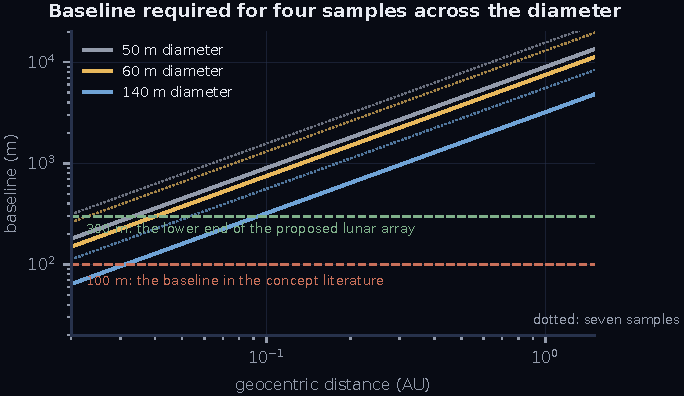
\includegraphics[width=\textwidth]{../figures/fig_shape_baseline.pdf}
\caption{The baseline required for four samples across the diameter, against
the geocentric distance, for three diameters. The 100-metre baseline of the
concept literature never reaches the requirement for the small class.}
\label{fig:shape-baseline}
\end{figure}

\section{The re-derivation of the concept study's own table}

The 2003 concept study for the Comet/Asteroid Protection System published a
table of the maximum baseline usable against a target's angular size, for
eight cases spanning a one-kilometre object at six astronomical units and a
50-metre object at 0.2 astronomical units.

The book's generator reproduces that table's maximum-baseline column from
the rule
\begin{equation}
B_{\max} = \frac{\lambda}{4\,\theta_{\mathrm{diam}}},
\label{eq:bmax}
\end{equation}
to within 0.71 per cent on all eight rows, and reproduces the precision
column as
\begin{equation}
\sigma_\theta = \frac{\lambda}{B\,\mathrm{SNR}}
\label{eq:precision}
\end{equation}
to within 2.21 per cent, with the signal-to-noise ratio of 7 given in the
source.

That the table reproduces does not mean the table is right for the purpose
the book needs. It means the table is internally consistent, and its
consistency lets us read off what it is actually describing.

\section{What the design point actually is}

The concept study's design point is a 100-metre baseline with three-metre
apertures at 750 nanometres, a fringe visibility of 0.5 and a visual
magnitude of 27.

Apply \eqref{eq:samples} to a 50-metre object with that baseline. At 0.1
astronomical units the object's angular diameter is 0.689 milliarcseconds
and the fringe spacing is 1.547 milliarcseconds, so
\begin{equation}
N = \frac{0.689}{1.547} = 0.45.
\end{equation}
At 0.2 astronomical units the angular diameter is 0.345 milliarcseconds and
the ratio is 0.22. In both cases \textbf{the target is smaller than half of
one fringe spacing}. The instrument is an astrometric centroid, and the
concept study says so itself: its stated purpose is ``a commensurate drop in
the orbit determination error''.

\begin{seamnote}{The 2024 and 2025 lunar interferometry literature is sized
for stars}
The recent lunar optical interferometry study proposes a 100-metre baseline
with 30-centimetre apertures over 450 to 850 nanometres, and the
Artemis-enabled stellar imager is a long-baseline ultraviolet and optical
instrument for stellar astrometry. Both are sized for milliarcsecond stellar
astrometry, and neither is an asteroid shape imager. Neither was intended to
be. The point of the re-derivation is not to accuse them of an error; it is
to establish that the lunar shape-imaging niche is unoccupied by the
literature, and that its baseline requirement is a kilometre-scale one.
\end{seamnote}

\begin{figure}[!htbp]
\centering
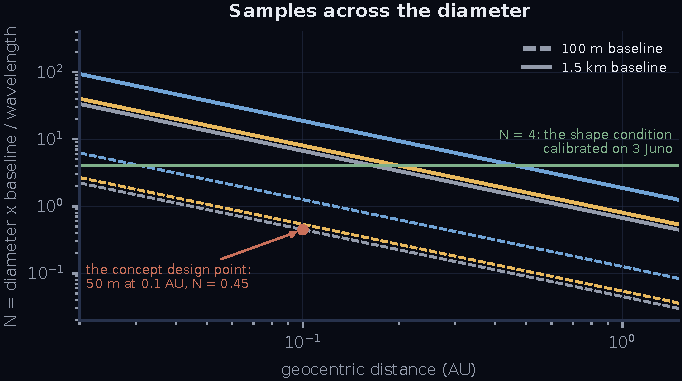
\includegraphics[width=\textwidth]{../figures/fig_samples.pdf}
\caption{Samples across the diameter against baseline and distance. A
hundred-metre baseline never reaches four samples for the 50-metre class at
0.2 astronomical units; a 1.5-kilometre baseline reaches it comfortably
across most of the class's distance range.}
\label{fig:samples2}
\end{figure}

\section{Visibility, and the over-resolution limit}

The other limit is the opposite one. A baseline much longer than the body
requires produces fringes whose visibility collapses, because the body's own
structure, rather than the instrument, then sets the visibility. The
uniform-disc model gives the visibility as
\begin{equation}
V = \left|\frac{2 J_{1}(x)}{x}\right|,
\qquad
x = \frac{\pi B\,\theta_{\mathrm{radius}}}{\lambda},
\label{eq:visibility}
\end{equation}
which the generator evaluates with the convergent series for the Bessel
function.

This is the over-resolution limit, and it is the reason the required baseline
must be \emph{matched} to the target rather than simply made long. The
usable baseline window for a target of a given angular size is bounded on
both sides: too short and the body is unresolved, too long and the fringe
visibility is gone.

\begin{table}[!htbp]
\centering
\small
\caption{The usable baseline window for the small class at 750 nanometres,
with four samples as the lower bound and a unit visibility as the upper.}
\label{tab:baseline-window}
\begin{tabularx}{\textwidth}{@{}P{0.77in}P{0.89in}P{1.04in}Y@{}}
\toprule
\rowcolor{panel}
\textbf{Diameter} & \textbf{Distance} & \textbf{Baseline window} &
\textbf{Comment} \\
\midrule
60 m & 0.2 AU & 1.5 to 1.9 km & the narrowest useful window in the class \\
\rowcolor{panel}
60 m & 0.5 AU & 3.7 to 4.4 km & \\
140 m & 0.2 AU & 0.6 to 0.8 km & \\
\rowcolor{panel}
140 m & 0.5 AU & 1.6 to 1.9 km & \\
\bottomrule
\end{tabularx}
\end{table}

The windows in \tabref{tab:baseline-window} are the reason the architecture
has to be an array with a choice of separations rather than a single
interferometer. A station that has to image a 60-metre object at 0.2
astronomical units and a 140-metre object at 0.5 astronomical units needs
baselines of very different lengths, and it needs to be able to select
between them on the timescale of a campaign.

\begin{deeper}{The visibility model this book does not have}
\eqref{eq:visibility} is a uniform-disc model, and the book says plainly
that it is not adequate for the resolved case. A genuinely resolved body
with limb darkening and surface contrast produces a visibility that is not
the uniform-disc function at all, and the fringe visibility of a real
asteroid at a matched baseline is a property of its albedo distribution
across the disc. The requirement for four samples is insensitive to this,
because it is set by the sampling condition rather than by the visibility.
The \emph{achievable precision} is not insensitive, and the book does not
claim a calibrated precision for a resolved target. What it does claim is
the requirement, which is what a programme would be specified against.
\end{deeper}

\begin{keytakeaways}
\item A shape image requires four samples across the diameter, which for the
60-metre class means baselines of 748 metres at 0.1 astronomical units and
3,740 metres at 0.5.
\item The concept study's own table reproduces as \(B_{\max} = \lambda/(4
\theta)\) to within 0.71 per cent, and its 100-metre design point puts the
50-metre class below half a fringe spacing.
\item The recent lunar interferometry literature is sized for stellar
astrometry, which leaves the asteroid shape-imaging niche unoccupied.
\item The usable baseline window is bounded on both sides, so the station has
to be an array with selectable separations rather than a single
interferometer.
\end{keytakeaways}


\part{The Moon}
\label{part:moon}
% =====================================================================
%  Chapter 21 — \idxw{Vantage}: What the Moon Sees That the Earth Does Not
% =====================================================================

\chapter{Vantage: What the Moon Sees That the Earth Does Not}
\label{ch:vantage}

The Moon is not a better telescope than the Earth. It is a different
environment, and three of its environmental differences are quantifiable and
favourable for the specific task this book has in mind. A fourth, which the
concept literature lists as a disadvantage, turns out on inspection to be an
advantage, and that reversal is the pivot on which the whole lunar case
turns.

\section{The sky turns twenty-seven times more slowly}

The Earth rotates once a day, and the sky turns with it at fifteen degrees
an hour. The Moon rotates once every 27.321661 days relative to the stars,
so the lunar sky turns at 13.176 degrees per day. The ratio is
\begin{equation}
\frac{15\ \mathrm{deg\,hr^{-1}}}{13.176\ \mathrm{deg\,day^{-1}}} = 27.4.
\label{eq:skyrate}
\end{equation}

\begin{figure}[!htbp]
\centering
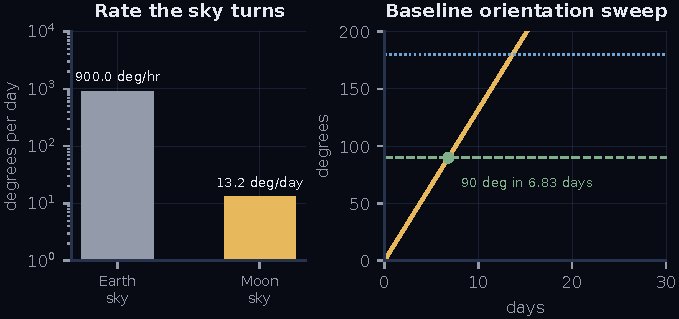
\includegraphics[width=\textwidth]{../figures/fig_rotation.pdf}
\caption{Left: the rate at which the sky turns on the Earth and on the Moon,
on a logarithmic scale. Right: the sweep of a fixed lunar baseline's
orientation, which reaches ninety degrees in under seven days.}
\label{fig:rotation}
\end{figure}

Three consequences follow, and they are of very different kinds.

The first is the observing window. A fixed station on the Earth sees a
target for as long as the target is above the horizon, which at a good
latitude and a good site is a few hours of usable time per night. A fixed
station on the Moon sees a target for as long as the target is above the
lunar horizon, and the lunar sky's slow rotation means that the target's
diurnal motion across the lunar sky is dominated by the target's own proper
motion rather than by the sky's rotation. The access windows are measured in
days rather than hours.

The second is the absence of tracking. Because the sky's rotation is slow,
the pointing is nearly fixed over a campaign, and the integration time is
limited by the target's own motion rather than by a mount. For an
interferometer, whose fringe acquisition needs a stable path difference over
the integration, this matters.

The third is the one the concept literature gets backwards.

\begin{deeper}{The rotation rate as a constraint and as an asset}
The 2003 concept study lists, among the disadvantages of a surface-fixed
interferometer, the fact that ``observations are constrained by the Moon's
rotation rate''. That is true and it is an advantage, because the same
document also states that ``having the interferometer fixed to the lunar
surface keeps the baseline very stable, reducing measurement uncertainties'',
and that ``two measurements at different baseline orientations
(\(\sim\)orthogonal) are required to derive the target's two-angle
position''.

Those two statements are in tension, and the resolution is arithmetic. A
fixed baseline on the Moon sweeps through ninety degrees of orientation in
\(90/13.176 = 6.83\) days. The orthogonal second orientation that the
concept study requires is therefore delivered automatically, within a week,
by the rotation itself, with no moving hardware and no propellant. On the
Earth, the same requirement would need a second instrument or a transport
delay.
\end{deeper}

\section{The Sun-ward blind zone}

The second advantage is geometrical and it is the discovery-side case.

A ground telescope cannot observe close to the Sun: atmospheric scattering
raises the sky background, and the solar avoidance constraints tighten. The
result is the blind zone that the 2026 study of near-Earth-object telescopes
for extreme environments calls the most critical limitation of ground-based
observatories, and it names the historical failures it has caused: 2008~TC3
and 2019~OK, and ``multiple other NEAs detected only days before their
closest approach to Earth''.

The lunar geometry relaxes the constraint. From a polar site\idx{Polar site}, where the Sun
stays low and the sky background is correspondingly low, an observer can see
close to the Sun. The same study publishes the resulting gain as a table of
first detectable distances and extra lead times.

\begin{figure}[!htbp]
\centering
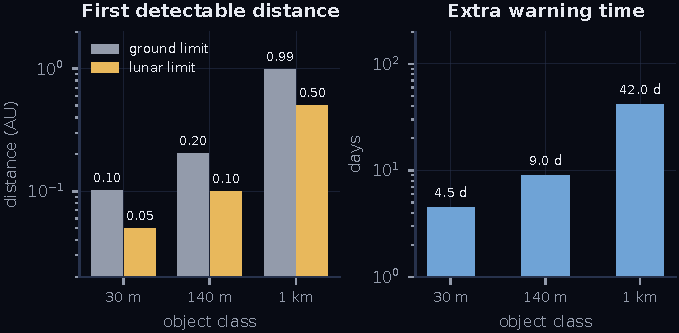
\includegraphics[width=\textwidth]{../figures/fig_sunward.pdf}
\caption{The Sun-ward gain, reconstructed from the published table. Left:
the first detectable distance from the ground and from a lunar observatory.
Right: the extra warning time, at a relative velocity of 20 kilometres per
second.}
\label{fig:sunward}
\end{figure}

\figref{fig:sunward} is worth reading carefully, because it is modest and
the book does not inflate it. A 30-metre object becomes detectable 0.05
astronomical units from the Sun and four to five days earlier. A
140-metre object becomes detectable at 0.10 astronomical units and about nine
days earlier. A one-kilometre object becomes detectable at 0.50 astronomical
units and about six weeks earlier.

Working backwards from the lead times, the ground limits the table implies
are about 0.10 astronomical units for the 30-metre class, 0.20 for the
140-metre class and 0.99 for the kilometre class.

Nine days is not a transformation of planetary defence. What it is, is the
only entry in the table that applies to objects the ground structurally
cannot reach, and it is the entry that matters for the population of Chapter
4: the objects that are still arriving at three thousand a year are the
small, near-Sun ones, and they are the ones the ground finds last.

\section{No atmosphere, and what that is worth}

The third advantage is the one the concept literature lists first, and it is
the least important for this book's proposal, for a reason worth stating.

With no atmosphere there is no scattered light and no airglow, so the diffuse
background at a dark polar site is the zodiacal light and the starlight
alone. The consequence can be computed from the target's own photometry. A
60-metre object at 0.2 astronomical units has an apparent magnitude of 17.2,
and once resolved, a surface brightness of 0.06 magnitudes per square
arcsecond --- about 22 magnitudes above the zodiacal background. At 1.0
astronomical unit its surface brightness is 3.55 magnitudes per square
arcsecond, still about 18 magnitudes above it.

The background is therefore not the constraint on a lunar optical
interferometer. The baseline is. This is worth saying because the intuitive
argument --- ``no atmosphere, so no seeing, so better images'' --- is true
and largely irrelevant to a sixty-metre object seen from a hundred million
kilometres.

\begin{table}[!htbp]
\centering
\small
\caption{The three lunar advantages, and what each one is actually worth
for this task.}
\label{tab:advantages}
\begin{tabularx}{\textwidth}{@{}P{1.33in}P{1.23in}Y@{}}
\toprule
\rowcolor{panel}
\textbf{Advantage} & \textbf{Worth} & \textbf{Comment} \\
\midrule
Slow sky rotation & high & day-long windows, no tracking, and the
orthogonal baseline orientation delivered within 6.83 days \\
\rowcolor{panel}
Sun-ward access & moderate & four to five days for a 30-metre object, nine
days for a 140-metre one \\
No atmosphere & low & the target is 18 to 22 magnitudes above the
background; the baseline is the constraint \\
\bottomrule
\end{tabularx}
\end{table}

\begin{keytakeaways}
\item The lunar sky turns twenty-seven times more slowly than the Earth's,
which gives day-long observing windows and no tracking requirement.
\item The same rotation delivers the orthogonal baseline orientation the
concept study requires within 6.83 days, with no moving hardware.
\item The Sun-ward gain is modest in absolute terms but reaches the only
population the ground structurally cannot see.
\item The absence of atmosphere is the least important of the three: the
target is 18 to 22 magnitudes above the zodiacal background.
\end{keytakeaways}

% =====================================================================
%  Chapter 22 — The \idxw{Baseline} the Moon Gives and the Baseline\idx{Baseline} It Does Not
% =====================================================================

\chapter{The Baseline the Moon Gives and the Baseline It Does Not}
\label{ch:baseline}

Chapter 20 established the requirement: an asteroid shape imager needs a
baseline\idx{Baseline} of hundreds of metres to a few kilometres, matched to the target's
angular size. This chapter asks whether the Moon can provide it, and the
answer is yes for a specific reason that has nothing to do with the Moon
being far away.

\section{The construction problem and the atmosphere problem}

A terrestrial optical array with a baseline\idx{Baseline} of a kilometre has three
simultaneous difficulties, and they are of different kinds.

The \emph{atmospheric} difficulty is that a kilometre of atmosphere is not a
stable optical element. The index of refraction along a kilometre of air
varies with temperature and pressure, and the path length between two
apertures separated by a kilometre changes by a comparable amount. The
optical path difference that an interferometer measures has to be stable to
a small fraction of a wavelength, and a kilometre of air is not.

The \emph{metrological} difficulty is that the two apertures must be
surveyed relative to each other to a fraction of the path stability
required, and a terrestrial baseline is subject to seasonal ground motion,
to thermal expansion of the structures that carry it, and to the slow
deformation of the crust.

The \emph{construction} difficulty is that a kilometre-long structure has to
be built, aligned and maintained on a surface that is not flat, and that
has to be done in a way that survives weather.

The important observation is that these three difficulties are not
independent. On the Earth they are coupled through the atmosphere: the
instrument has to be built on the ground because the atmosphere is above the
ground, and it has to be metrologically stable because the atmosphere is
changing, and it has to be maintained because the ground moves.

On the Moon, the coupling is broken. The ground is rigid and airless and
slowly rotating, with no thermal expansion of a truss to worry about and no
weather and no hydrology. A baseline on the Moon is defined by the distance
between two surveyed anchor points, and the surveying problem is a lunar
geodesy problem rather than an optical-metrology\idx{Metrology} problem.

\begin{seamnote}{This is the defensible lunar claim, and it is narrow}
Not ``the Moon offers a unique vantage point''. Not ``the Moon is closer to
the objects''. The claim is that the lunar surface is the only site where
the kilometre-scale baseline that shape imaging requires can be built,
because the construction problem can be separated from the atmosphere
problem. That is a much smaller claim than the concept literature's, and it
is the one that survives the arithmetic.
\end{seamnote}

\section{The stability argument, and what it is worth}

The concept literature's stability statement is worth reading precisely:
``having the interferometer fixed to the lunar surface keeps the baseline
very stable, reducing measurement uncertainties''.

The physical content is this. A baseline fixed to a rigid, airless body
does not move relative to the body, and the body's orientation relative to
the distant stars is predictable from its rotation. The vector from one
aperture to another therefore has a known direction to a precision set by
the anchor-point survey, and the direction is not corrupted by the
atmosphere's index variations or by the ground's seasonal motion.

What the argument does not say is that the Moon is a good place to build
anything. The regolith is abrasive, the night is long, and the dust is a
mitigation problem with a demonstrated but unproven long-term solution.
Chapter 24 takes the engineering envelope apart. The point of the stability
argument is narrower: it identifies a property that a terrestrial array
cannot have, and that a lunar array can have at a scale that matters.

\section{The baseline the Moon does not give}

Two things have to be said about what the lunar surface does not provide,
and the first of them is the more awkward of the two.

It does not provide the length of baseline that the radio interferometry of
Chapter 8 used. The Very Long Baseline Array reached 1,200 to 2,300
kilometres with the planets as reflectors, and the effective baseline of
that technique came from the Earth's own diameter. A lunar surface array
cannot reach that, and does not need to: the optical wavelength is 750
nanometres rather than 4.2 centimetres, and the required baseline is
correspondingly shorter.

It does not provide proximity. The Moon is not closer to the near-Earth
objects than the Earth is; at a close approach it may be closer or
considerably farther, depending on the geometry. The lunar advantage is
not range. It is the stability of the baseline, the length of the observing
window, and the Sun-ward access.

\begin{table}[!htbp]
\centering
\small
\caption{The three lunar advantages against the terrestrial alternative, and
what each is worth to the shape measurement.}
\label{tab:baseline-compare}
\begin{tabularx}{\textwidth}{@{}P{1.22in}P{1.34in}Y@{}}
\toprule
\rowcolor{panel}
\textbf{Property} & \textbf{Terrestrial array} & \textbf{Lunar array} \\
\midrule
Baseline length & a few hundred metres is already at the limit & a few
hundred metres to kilometres is a construction problem, not an optical one \\
\rowcolor{panel}
Path stability & atmospheric and seasonal & set by the anchor-point survey
alone \\
Observing window & hours, per night & days \\
\rowcolor{panel}
Orthogonal orientation & a second instrument, or a transport delay & 6.83
days, delivered by the rotation \\
Sun-ward access & structurally excluded & available at a polar site \\
\bottomrule
\end{tabularx}
\end{table}

\section{The array the requirement implies}

Putting Chapter 20's requirement together with this chapter's engineering
gives the array specification, and it is worth stating in the form a
programme would use.

The array is a set of fixed apertures at surveyed separations spanning
roughly 300 metres to 3 kilometres, at a site with a low horizon in the
direction of the objects of interest. The station selects the aperture pair
whose separation matches the target's angular size, so that the number of
samples across the diameter is in the range four to seven.

\begin{table}[!htbp]
\centering
\small
\caption{The matched separations the array has to provide, for the class of
interest, at four samples and seven samples across the diameter.}
\label{tab:array-separations}
\begin{tabularx}{\textwidth}{@{}P{0.78in}P{0.90in}P{1.02in}Y@{}}
\toprule
\rowcolor{panel}
\textbf{Diameter} & \textbf{Distance} & \textbf{Four samples} &
\textbf{Seven samples} \\
\midrule
60 m & 0.1 AU & 748 m & 1,309 m \\
\rowcolor{panel}
60 m & 0.2 AU & 1,496 m & 2,618 m \\
60 m & 0.5 AU & 3,740 m & 6,545 m \\
\rowcolor{panel}
140 m & 0.1 AU & 321 m & 561 m \\
140 m & 0.2 AU & 641 m & 1,122 m \\
\rowcolor{panel}
140 m & 0.5 AU & 1,603 m & 2,805 m \\
\bottomrule
\end{tabularx}
\end{table}

The separations in \tabref{tab:array-separations} span a factor of twelve,
from 321 metres to 6,545 metres, and they change with the distance to the
target, which changes with the object's orbit and therefore with the season.
A single-baseline instrument cannot serve this table. An array with a
discrete set of anchor separations can, and the selection rule that chooses
the pair is a rule about the target, not about the instrument.

\begin{keytakeaways}
\item A terrestrial kilometre-scale array is simultaneously an atmospheric, a
metrological and a construction problem; on the Moon the construction
problem separates from the atmosphere problem.
\item The Moon does not give a longer baseline than the radio technique of
Chapter 8, and it does not give proximity; it gives stability, window length
and Sun-ward access.
\item The baseline orientation requirement is met by the Moon's own rotation
in 6.83 days, with no moving hardware.
\item The array must offer separations from 321 metres to 6,545 metres, which
means selectable anchor pairs rather than a single interferometer.
\end{keytakeaways}

% =====================================================================
%  Chapter 23 — The Thermal and Power Budget
% =====================================================================

\chapter{The Thermal and Power Budget}
\label{ch:thermal-budget}

The mid-infrared channel is where the lunar proposal is weakest, and the
arithmetic is unusually clean. This chapter works through it, because a
reader is entitled to know where the argument loses, and because the place
it loses is a place where a better platform already exists.

\section{The ground is brighter than the target}

Sunlit lunar regolith reaches about 390 kelvin. By Wien's displacement law,
a blackbody at that temperature radiates with its peak at
\begin{equation}
\lambda_{\mathrm{peak}} = \frac{2898\ \mu\mathrm{m\,K}}{390\ \mathrm{K}}
= 7.43\ \mu\mathrm{m},
\label{eq:wien}
\end{equation}
which is squarely inside the 5 to 14 micrometre band in which asteroid
thermal emission is measured. At 10 micrometres, with an emissivity of 0.9,
that regolith radiates 27.5 watts per square metre per steradian per
micrometre.

The target's own thermal disk is dimmer. A Lambertian sphere's resolved
surface brightness at 10 micrometres is \(B_\lambda(T_{\mathrm{sub}})/4\),
independent of its distance from the observer, and the subsolar temperature
scales as \(278\ \mathrm{K}\times r^{-1/2}\). The ratio of the target's disk
to the sunlit ground is therefore

\begin{figure}[!htbp]
\centering
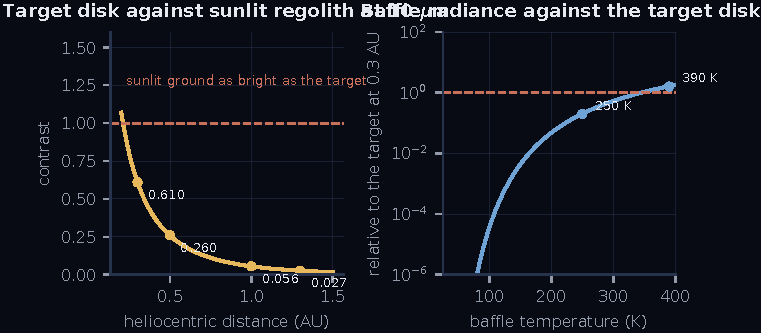
\includegraphics[width=\textwidth]{../figures/fig_mir.pdf}
\caption{Left: the contrast between a target's own thermal disk and the
sunlit lunar ground, against heliocentric distance. Below one everywhere.
Right: the radiance of a baffle at a range of temperatures against the
target's disk. The foreground is the telescope structure, not the ground.}
\label{fig:mir}
\end{figure}

\begin{table}[!htbp]
\centering
\small
\caption{Contrast between the target's thermal disk and sunlit regolith at
10 micrometres.}
\label{tab:mir-contrast}
\begin{tabularx}{\textwidth}{@{}P{1.32in}P{1.24in}Y@{}}
\toprule
\rowcolor{panel}
\textbf{Heliocentric distance} & \textbf{Contrast} & \textbf{Reading} \\
\midrule
0.3 AU & 0.61 & the target's disk is 61 per cent of the ground's \\
\rowcolor{panel}
0.5 AU & 0.26 & the ground is four times brighter \\
1.0 AU & 0.055 & the ground is eighteen times brighter \\
\rowcolor{panel}
1.3 AU & 0.027 & the ground is thirty-seven times brighter \\
\bottomrule
\end{tabularx}
\end{table}

In every heliocentric distance at which these objects are scientifically
interesting, the sunlit lunar ground is brighter than the asteroid's own
thermal emission. \tabref{tab:mir-contrast} is the first half of the case
against a lunar mid-infrared channel.

\section{The foreground is the telescope, not the ground}

The second half is more interesting, because it changes the engineering
conclusion rather than just the feasibility one.

The ground is not what the instrument looks at. The instrument looks along a
baffle or a sunshade, and the baffle has its own temperature and its own
radiance. A baffle at 390 kelvin is 1.6 times brighter than the target's
disk; a baffle at 250 kelvin is a factor of five fainter than the target and
entirely workable; a baffle at 40 kelvin is smaller by seventeen orders of
magnitude.

So the lunar mid-infrared channel is not forbidden by the background. It is
a cryogenic-optics problem: the optics must be held near 40 kelvin while
sitting on 390 kelvin regolith, with no atmosphere to reject heat into and
no radiative path other than deep space.

\begin{deeper}{What this means for the proposal}
The difference between a background problem and an engineering problem is the
difference between a channel that cannot exist and a channel that costs a
cryostat and ten kilowatts. The book states the second, because the second
is what an engineering study would have to answer. But the answer is
expensive, and Chapter 26 shows that a platform already exists that answers
it for less.
\end{deeper}

\section{The two cures, and their prices}

The cold cure is a permanently shadowed region, where the ground sits at 25
to 40 kelvin. The foreground there is lower than the target's disk by
seventeen to nineteen orders of magnitude, so the thermal problem vanishes
completely.

The price is that a permanently shadowed region receives no sunlight and
therefore has no power. The power cure is published by NASA: combining
regenerative fuel cells with a vertical solar array technology ``enables
supply and recharge of 10KW of power to permanently shadowed regions on the
Moon''. The deployable mast concept is the same idea in hardware form.

The price of the power cure is a 10 kilowatt-class power system, a cryogenic
instrument, and a night that runs for 328 hours. The instrument survival
temperatures are about 100 kelvin, and a seven kilowatt-hour battery is
needed to carry a spectrometer through the lunar night.

\begin{table}[!htbp]
\centering
\small
\caption{The mid-infrared channel: what it costs on the Moon, and what the
comparison platform already provides.}
\label{tab:mir-comparison}
\begin{tabularx}{\textwidth}{@{}P{1.24in}P{1.32in}Y@{}}
\toprule
\rowcolor{panel}
\textbf{Parameter} & \textbf{Lunar surface} & \textbf{Sun-Earth L1} \\
\midrule
Aperture & as chosen & 0.5 m, already specified \\
\rowcolor{panel}
Band & 5 to 14 micrometres & 4 to 5.2 and 6 to 10 micrometres \\
Detector temperature & about 40 K & 40 K \\
\rowcolor{panel}
Passive cooling & requires a permanently shadowed region & a space
radiator, no regolith, no dust, no night \\
Status & a concept & two funded missions \\
\bottomrule
\end{tabularx}
\end{table}

\tabref{tab:mir-comparison} is the comparison that decides the channel. The
European Space Agency's NEOMIR concept has a 50-centimetre telescope
passively cooled below 60 kelvin with detectors at 40 kelvin, a 6 to 10
micrometre band, a 30 to 70 degree solar elongation field of regard and no
atmosphere, no dust and no night. NASA's NEO Surveyor has a 50-centimetre
telescope on a halo orbit at Sun-Earth L1 with 4 to 5.2 and 6 to 10
micrometre channels. Both are the same aperture, both at 40 kelvin, and
neither has to survive regolith.

\section{The verdict}

The verdict on the thermal channel is therefore not that the Moon cannot do
it. It is that a space telescope does it better and more cheaply, and the
comparison decides it.

That is a loss, and the book records it as a loss. The proposal that follows
in Chapter 25 has no mid-infrared channel, and the optical channel is the
one it carries. This is not a retreat from the original concept; it is the
consequence of taking the arithmetic seriously, and it makes the proposal
smaller, cheaper and more defensible.

\begin{keytakeaways}
\item Sunlit regolith at 390 kelvin is brighter than the target's own
thermal disk at every heliocentric distance of interest, with contrasts
from 0.61 down to 0.027.
\item The real foreground is the baffle, which is 1.6 times the target at
390 kelvin and seventeen orders of magnitude below it at 40 kelvin, so the
channel is an engineering problem rather than an impossibility.
\item The cold cure is a permanently shadowed region, which has no power,
and the power cure is a 10 kilowatt-class system that has to survive a
328-hour night.
\item The comparison decides the channel: a 0.5-metre telescope at
Sun-Earth L1 is already specified for it, at 40 kelvin, with no regolith.
\end{keytakeaways}

% =====================================================================
%  Chapter 24 — \idxw{Dust}, \idxw{Night} and the Engineering Envelope
% =====================================================================

\chapter{Dust, Night and the Engineering Envelope}
\label{ch:envelope}

The lunar concept has two objections that have been attached to it since
the beginning: the dust\idx{Dust} and the night. The dust\idx{Dust} objection has moved
furthest, because a mitigation technology that was a proposal when the
concept was written has now been demonstrated on the Moon. The night\idx{Night}
objection has not moved at all, because it is arithmetic.

\section{Dust, and the demonstration that changed its status}

The \idxw{Electrodynamic Dust Shield} lifts and clears regolith from surfaces using
a patterned electrode array generating a non-uniform electric field. It was
demonstrated on the lunar surface during Firefly Aerospace's Blue Ghost
Mission 1 in 2025, raising its technology readiness level from 5 to 7, with
a camera-lens clearing efficiency estimated at 96.6 per cent. NASA's current
dust\idx{Dust} mitigation catalogue lists it at that level for the Moon.

Two things should be said about it, and the second is the important one.

The first is that the dust objection has changed character. It is no longer
an open question whether the dust can be moved off an optic. It is a
question about how long an optic can be kept clean, on a surface where the
optics cannot be serviced for years, with a mitigation that NASA's own
roadmap cautions ``should not be the only tool in our toolbox''.

The second is that a shield is a mitigation for dust \emph{on a surface}.
Nothing in the published work shows that it can protect the primary mirror of
an interferometric aperture, or the baffle edges of a kilometre-scale array
spread over three kilometres of ground, or the coatings on a delay line that
has to hold a path difference to a fraction of a wavelength. The
demonstration was a camera lens on a lander.

\begin{seamnote}{The distinction the proposal has to live with}
A camera lens on a lander is a flat, exposed, near-surface, replaceable
optical element. A kilometre-scale array is a set of apertures on anchor
points, each with its own baffle, and the array is not replaceable. The
dust mitigation that has been demonstrated addresses the first problem and
not the second. The book does not claim otherwise; it claims that the
engineering envelope is closed enough to be worth designing against, and
that the residual dust risk is one of the things that would have to be
managed by the baseline selection rule rather than by cleaning.
\end{seamnote}

\section{The night, which is arithmetic}

The lunar night\idx{Night} at a polar site runs for about 328 hours, or thirteen and a
two-thirds days. Over that period a thermally exposed instrument drifts
towards the temperature of its surroundings, and the published engineering
figures for a thermally controlled payload at the south pole give survival
temperatures of about 100 kelvin and a seven kilowatt-hour battery to carry
a spectrometer through the night.

Three consequences follow for the proposal of Chapter 25.

The optical channel's baffle has to be held below about 250 kelvin for the
background arithmetic of Chapter 23 to work, and that is an insulation
problem rather than a cryogenics problem. The mid-infrared channel, which
needs 40 kelvin, would need the permanently shadowed region and therefore
the full power architecture. This is precisely why the proposed architecture
has no mid-infrared channel: the night\idx{Night} is what makes the cryogenic option
expensive, and the optical option is cheap by comparison.

The instrument cannot be pointed at the Sun during the night in any case,
because the Sun is below the horizon at a polar site for the whole of it.
The operational consequence is that the night is not a period of reduced
service but a period of no service, and that the campaign scheduling has to
account for it.

And the station's power has to come from somewhere that is not the
illuminated surface, or from storage that lasts the night. The published
answer --- regenerative fuel cells combined with vertical solar arrays,
delivering 10 kilowatts to permanently shadowed regions --- is a
kilowatt-class architecture for an instrument that does not need kilowatts.

\begin{table}[!htbp]
\centering
\small
\caption{The engineering envelope, item by item, with the status each item
has reached.}
\label{tab:envelope}
\begin{tabularx}{\textwidth}{@{}P{1.37in}P{1.19in}Y@{}}
\toprule
\rowcolor{panel}
\textbf{Item} & \textbf{Status} & \textbf{What the book claims} \\
\midrule
Atmospheric seeing & solved & no atmosphere at all \\
\rowcolor{panel}
Baseline stability & solved & a rigid, airless, slowly rotating body \\
Dust & mitigated & a flight demonstration at TRL 7; the long-term case for
a kilometre-scale array is open \\
\rowcolor{panel}
Night survival & arithmetic & 328 hours, 100 K survival, a 7 kWh battery \\
Power & published & 10 kW to permanently shadowed regions \\
\rowcolor{panel}
Thermal background & closed for optical & the baffle at 250 K; the
mid-infrared channel loses to L1 \\
Observing window & quantified & 6.83 days for the orthogonal orientation \\
\bottomrule
\end{tabularx}
\end{table}

\section{What the envelope permits}

The envelope in \tabref{tab:envelope} permits a specific instrument and
forbids others. It permits a visible-light interferometer with a thermally
controlled baffle, a surveyed array of anchor points, a service that operates
in daylight near the pole, and a campaign structure that uses the slow
rotation of the sky.

It forbids a mid-infrared channel, a cryogenic payload in an illuminated
site, and a service that depends on a continuously available sky. And it
imposes the constraint that the station's duty cycle is set by the
twenty-eight-day lunar cycle rather than by the observing target.

That last point is worth stating as a number, because it is the number that
the campaign rate in the next chapter depends on. The station can observe
for roughly half of each synodic month, at the pole, and it can observe
objects that are near the Sun at all, and it cannot observe through the
night. The net effect on the annual service rate is a factor that the
book's generator folds into its overhead allowance.

\begin{keytakeaways}
\item Dust mitigation has been demonstrated on the Moon at TRL 7 with a
96.6 per cent camera-lens clearing efficiency, but it has not been
demonstrated for a kilometre-scale array.
\item The night runs for 328 hours, with survival temperatures near 100
kelvin and a 7 kilowatt-hour battery.
\item The envelope permits a visible-light instrument with a baffle at about
250 kelvin and forbids a mid-infrared channel in an illuminated site.
\item The duty cycle is set by the lunar cycle rather than by the target,
and it is the single largest term in the overhead allowance.
\end{keytakeaways}

% =====================================================================
%  Chapter 25 — The \idxw{Array} Architecture and the \idxw{Service} Model
% =====================================================================

\chapter{The Array Architecture and the Service Model}
\label{ch:architecture}

The arithmetic of the previous five chapters constrains the architecture
more tightly than a concept paper would suggest, and the constraint is
productive: it removes the mid-infrared channel, it fixes the baseline
range, it sets the wavelength, and it makes the station a service\idx{Service} rather
than an instrument. This chapter assembles the result.

\section{Four elements}

\subsection{Site and plant}

A sunlit ridge or crater rim at the lunar south pole, within a few hundred
metres of a permanently shadowed region used for services and power
conversion, so that heat rejection and power generation are decoupled from
the aperture geometry. NASA's own lunar surface technology catalogue treats
10 kilowatts of power delivered to permanently shadowed regions as an
available capability.

The optical channel requires only that the baffle and sunshade be held
below about 250 kelvin, which is an insulation problem. A mid-infrared
channel is optional, expensive, and on the evidence of Chapter 23 it loses to
Sun-Earth L1, so the proposed architecture does not carry one.

\subsection{The array}

A distributed set of fixed apertures on baselines of 300 metres to
3 kilometres, each fixed to a surveyed anchor point, with at least two
orthogonal orientations because the baseline orientation sweeps with the
Moon's rotation and a single orientation cannot deliver a two-angle
position.

The baseline is set by geology rather than by metrology. The requirement is
the anchor-point separation and its survey to sub-millimetre over kilometres,
which is a lunar geodesy problem rather than an optical-metrology problem.
The separations have to be discrete and selectable, because
\tabref{tab:array-separations} in Chapter 22 shows the matched baseline
changing with the target's distance by a factor of twelve across the
class.

\subsection{Wavelength and channels}

Visible, centred near 750 nanometres, which is where the 50 to 140 metre
class is brightest --- apparent magnitudes from 12.4 to 25.8 across the class
and the 0.1 to 1.3 astronomical unit range --- and where the concept study's
own sensitivity analysis sits.

The fringe visibility in the resolved regime is set by the body's limb
profile and surface contrast rather than by a uniform disc, which is why the
literature finds that a Minnaert model with multiple baselines is necessary
for a few per cent on size. The book's own generator uses the uniform-disc
model and says so in Chapter 20; the requirement it derives is insensitive
to the model, and the achievable precision is not.

A photometric and low-resolution spectroscopic channel on the same apertures
supplies the albedo prior and the taxonomy the thermal solution requires,
and the lightcurve that fixes the rotation period.

\subsection{Service}

This is the element with the highest verified value and the lowest technical
difficulty, and it is where the owner's original concept finds its proper
place.

The station is not a survey. It is a named-target characterisation service\idx{Service}
with a bounded turnaround, and each request returns a resolved shape model,
a pole and period, the epoch-corrected astrometry, and the photometry
needed for the albedo prior.

The requests are generated by an automated alert path\idx{Alert path} from the risk list to
the instrument, because the documented failure of the 2024~YR4 episode was
that ``no automated system currently alerts physical characterization
sites'', and the 2025 experiment with 2025~FA22 showed that such an alert is
operationally simple.

\begin{seamnote}{What the beam to Earth became}
The original concept carried a beam from the Moon to the Earth, and the
instinct behind it was correct: something had to connect the risk list to
an instrument that could respond. The record says the connection was the
missing piece. The beam is therefore re-purposed as an alerting and
scheduling path rather than as a ranging channel, because the ranging
channel turns out to be the weaker of the two claims, and because the
documented failure was a routing failure rather than a sensing failure.
\end{seamnote}

\section{The service rate, and what it means}

The service model has a number attached to it, and the number is what makes
the proposal honest.

A fixed station needs a 90-degree sweep of its baseline orientation to
deliver the two orthogonal measurements an interferometric position
requires, and the Moon's rotation takes 6.83 days to deliver that sweep.
Allowing thirty per cent of the time for overhead --- for the night, for
dust events, for maintenance, for scheduling conflicts --- one station runs
about 37 campaigns a year.

\begin{table}[!htbp]
\centering
\small
\caption{The service rate against the demand, and the coverage it buys.}
\label{tab:service}
\begin{tabularx}{\textwidth}{@{}P{1.56in}P{1.00in}Y@{}}
\toprule
\rowcolor{panel}
\textbf{Quantity} & \textbf{Value} & \textbf{Source} \\
\midrule
Orientation sweep & 6.83 days & the Moon's sidereal rotation \\
\rowcolor{panel}
Campaigns per year & 37 & 30 per cent overhead allowance \\
New 140 m objects per year & 342 & CNEOS, 2025 \\
\rowcolor{panel}
Annual coverage of the arrival rate & 10.9 per cent & the two above \\
Known 140 m objects & 11,725 & CNEOS, 22 November 2026 \\
\rowcolor{panel}
Years to clear the known catalogue & 313 & the two above \\
\bottomrule
\end{tabularx}
\end{table}

\tabref{tab:service} is the number that decides what the station is. It is
not a census machine. It cannot be, and no design change to the optics
changes the arithmetic, because the binding constraint is the rotation rate
and not the instrument.

\begin{deeper}{The rate against the backlog is the wrong comparison, and the
book says so}
Three hundred and thirteen years to clear the known catalogue sounds like a
disqualification, and in a planning document it would be. But the comparison
is wrong, for the reason Chapter 4 established: the gap is not discovery and
the station is not a census. The correct comparison is against the objects
whose characterisation changes an outcome --- the ones that will return, the
ones whose keyhole sits in the tail, the ones whose energy decides a
hazard class. That population is orders of magnitude smaller than 11,725,
and the selection rule of Chapter 30 defines it. A capability that serves
the decisive objects at ten per cent of the annual flow, with a turnaround
of days rather than years, is a triage capability, and triage is what the
gap requires.
\end{deeper}

\section{Why the service model is the load-bearing element}

It is worth being explicit about which of the four elements carries the
argument, because it is not the array.

The array is the technically interesting element and it is the one the
concept literature has already proposed. The wavelength and channels follow
from the photometry. The site and plant follow from the thermal budget.

The service model is the one that makes the whole thing an instrument rather
than an experiment, and it is the one with the smallest technical difficulty
and the largest verified value. The documented failure mode of the 2024~YR4
episode was that the observers of the object did not know it had reached
Torino Level 1. The documented capability gap is that no automated system
alerts physical characterisation sites. The documented demonstration that
the gap is closable is the 2025~FA22 alert exercise.

A station that returns a resolved shape, a pole and a period within days
of a request, triggered automatically by the risk list, is a service. A
station that observes what it can see is an experiment.

\begin{keytakeaways}
\item The architecture is a site, an array of surveyed anchors, a visible
channel with a photometric and spectroscopic companion, and a service.
\item The service returns a resolved shape, a pole and period, the astrometry
and the photometry, on a bounded turnaround, triggered by the risk list.
\item The rate is 37 campaigns a year, 10.9 per cent of the annual arrival
rate of the hazard class, and 313 years to clear the known catalogue.
\item The service model, not the optics, is the element that closes the
documented gap and that the 2025 alert exercise shows to be simple.
\end{keytakeaways}


\part{The Alternatives and the Rule}
\label{part:alternatives}
% =====================================================================
%  Chapter 26 — The Space Telescopes and What They Do Not Carry
% =====================================================================

\chapter{The Space Telescopes and What They Do Not Carry}
\label{ch:space-telescopes}

A proposal for the Moon is only as good as its comparison with what already
exists. The comparison is more favourable than expected in one respect and
less in another, and the row that decides the argument is not the row anyone
would have guessed.

\section{What is funded}

Two space telescopes carry the mid-infrared channel, and both are specified
in enough detail to be compared with a lunar proposal rather than guessed
at.

NASA's \idxw{NEO Surveyor} will operate a 50-centimetre telescope on a halo orbit\idx{Halo orbit} at
Sun-Earth L1, with 4 to 5.2 and 6 to 10 micrometre channels, surveying 45
to 120 degrees of solar elongation\idx{Elongation} and plus or minus 40 degrees of ecliptic
latitude on a roughly 13-day cadence.

The European Space Agency's \idxw{NEOMIR} concept has a 50-centimetre telescope
passively cooled below 60 kelvin with detectors at 40 kelvin, a 6 to 10
micrometre band, a 30 to 70 degree solar elongation\idx{Elongation} field of regard, and no
atmosphere, no dust and no night. It is at the concept phase A stage, with
an early-2030s date.

Both produce the same observable: an integrated thermal flux, from which a
diameter follows. Neither produces a shape, a spin state or a mass.

\section{The white paper that left the thermal channel to the ground}

The third entry is the one that settles the comparison, and it is a 2026
document rather than a legacy concept.

The white papers for a 3.5-metre segmented-mirror robotic space telescope
describe a baseline that spans 0.2 to 1.5 micrometres and that explicitly
excludes the mid-infrared. The stated architecture is that ``coordinated
ground-based mid-infrared telescopes provide the thermal fluxes required to
infer diameter and albedo, while the space mission supplies contemporaneous
reflected-light measurements and observing geometry''.

That is a division of labour decided by the people designing the most
capable space telescope now under study. The reflected-light channel, the
astrometric channel and the rotational channel are kept; the thermal channel
is handed to the ground.

\begin{table}[!htbp]
\centering
\small
\caption{The platform comparison: what each platform produces, the
population it reaches, and the limit that binds it.}
\label{tab:platforms}
\begin{tabularx}{\textwidth}{@{}P{1.28in}P{1.28in}Y@{}}
\toprule
\rowcolor{panel}
\textbf{Platform} & \textbf{Observable and population} & \textbf{Binding
limit} \\
\midrule
NEO Surveyor\idx{NEO Surveyor}, L1, 0.5 m & integrated thermal flux to a diameter; the whole
discovery stream at a 13-day cadence & diameter only; no shape, no spin \\
\rowcolor{panel}
NEOMIR\idx{NEOMIR}, L1, 0.5 m & as above, at 30 to 70 degrees elongation\idx{Elongation}, early 2030s &
as above; and it is not yet a mission \\
3.5 m segmented-mirror space telescope & resolved photometry, astrometry and
rotation; survey plus rapid response & no mid-infrared channel; relies on
ground mid-infrared \\
\rowcolor{panel}
Ground survey and follow-up & astrometry, lightcurve, photometry; thousands
of objects & unresolved; about 15 per cent with spectra \\
Ground adaptive optics & resolved shape & only at close approach; the wrong
phase angle wastes the window \\
\rowcolor{panel}
Ground bistatic radar & three-dimensional shape, spin, delay-Doppler; more
than fifty objects since 2015 & the echo falls as the fourth power of
distance \\
Lightcurve inversion & spin, pole and a convex shape; about 25,000 models &
the convex hull, and low-order shape only \\
\rowcolor{panel}
Low-Earth-orbit characterisation constellation & visible and near-infrared
characterisation & proposed; constrained by orbit and by brightness \\
Lunar surface array & resolved shape, spin, pole and astrometry; a named
target on demand & needs a kilometre-scale baseline; dust; night \\
\bottomrule
\end{tabularx}
\end{table}

\tabref{tab:platforms} is the manager's comparison table, and every row in
it is a platform that exists, is specified, or has been proposed with
enough detail to compare. The lunar row is the last, and it is the only one
whose binding limit is a construction problem rather than an observing
condition.

\section{The gap that has a shape}

The most capable space telescope concept now under study has chosen the
reflected-light channel for itself and left the thermal flux to the ground.

That is a division of labour with a consequence, and it is worth stating
plainly: it is not that nobody will fly the thermal channel. NEO Surveyor
and NEOMIR will. It is that the \emph{resolved, reflected-light, shape}
channel is not currently served by any space observatory, and that the
ground's contribution to it is smaller than a hundred models across the
entire history of the field.

\begin{table}[!htbp]
\centering
\small
\caption{Where the shape channel currently stands.}
\label{tab:shape-channel}
\begin{tabularx}{\textwidth}{@{}P{1.57in}P{0.99in}Y@{}}
\toprule
\rowcolor{panel}
\textbf{Provider} & \textbf{Models} & \textbf{Status} \\
\midrule
Space telescope, reflected light & none in service & the 3.5 m concept
excludes the mid-infrared and carries no shape programme \\
\rowcolor{panel}
Ground adaptive optics & a handful & close approach, good phase angle \\
Interferometry & fewer than ten, with a hundred projected & terrestrial
baselines of 1,200 km at radio wavelengths \\
\rowcolor{panel}
Fly-by imaging & six & one per multi-billion-dollar mission \\
Lightcurve inversion & about 25,000 & convex hulls \\
\bottomrule
\end{tabularx}
\end{table}

The shape channel is the one place where the portfolio is thinnest, and it
is the channel that the accounting chain runs through. The thermal channel
is well served, by two funded missions. The astrometric channel is
excellently served. The shape channel is served by six spacecraft and
several hundred ground images.

\section{What the space comparison decides and what it does not}

The comparison decides the thermal channel, and it decides it against the
Moon: a 0.5-metre telescope at Sun-Earth L1, already funded for the
thermal flux, at 40 kelvin, with no regolith and no dust, is a better
instrument for that channel than anything the proposal of Chapter 25 could
be built.

The comparison does not decide the shape channel, because no space
observatory is assigned to it.

\begin{keytakeaways}
\item Two funded space missions carry the mid-infrared channel, and the
flagship reflected-light space telescope concept has deliberately left that
channel to the ground.
\item No space observatory currently carries the resolved shape channel, and
the ground's contribution to it is a handful of close-range images and a
projected hundred interferometric models.
\item The comparison therefore decides the thermal channel against the Moon
and leaves the shape channel unassigned.
\item The portfolio is not thin everywhere: it is thin in exactly the place
the accounting chain runs through.
\end{keytakeaways}

% =====================================================================
%  Chapter 27 — Bistatic Radar and the Australian Record
% =====================================================================

\chapter{Bistatic Radar and the Australian Record}
\label{ch:bistatic-radar}

Radar is the instrument that closes the whole accountability chain, and the
strongest demonstration of it in the world is a pair of Australian radio
telescopes. This chapter takes the technique at its best, because a
comparison that only examines the competitors at their weakest is not a
comparison.

\section{What bistatic radar buys}

A single radar dish transmits and receives. The echo's delay gives the
range to the target and its Doppler shift gives the line-of-sight velocity;
together they reconstruct a three-dimensional shape, and the radar
cross-section gives the size.

A bistatic system separates the two functions. One station transmits and
another receives, and the geometry between them is the baseline. The
advantages are a much longer effective baseline, a different signal-to-noise
regime, and --- importantly for this book --- the possibility that one of the
two stations is not a radio telescope at all.

\section{The Australian record}

The demonstration record is the \idxw{Green Bank Telescope} and the \idxw{Parkes}
observatory used as a bistatic pair, with the Effelsberg 100-metre telescope
contributing in some campaigns. More than fifty near-Earth objects have been
characterised since 2015, including delay-Doppler images and polarimetric
measurements.

The polarimetry is the part that matters most for this book, because it is a
direct diagnostic of the surface state and therefore of the density question
that Chapter 7 identified as the second half of the energy gap. A radar
echo that is polarised in a particular way is a surface that is consolidated
rather than particulate, and that is a statement about the bulk density.

The delay-Doppler images are the part that matters for the shape, because
they are three-dimensional without a convexity assumption.

\begin{table}[!htbp]
\centering
\small
\caption{What the bistatic record delivers, and what limits it.}
\label{tab:bistatic}
\begin{tabularx}{\textwidth}{@{}P{2.57in}Y@{}}
\toprule
\rowcolor{panel}
\textbf{Quantity} & \textbf{Status} \\
\midrule
Objects characterised & more than fifty since 2015 \\
\rowcolor{panel}
Shape & three-dimensional, from delay-Doppler inversion, with no convexity
assumption \\
Polarimetry & a direct surface-state diagnostic and therefore a density
diagnostic \\
\rowcolor{panel}
Selection & only radar-crossing objects, and only at close range \\
Sensitivity growth & three times the Green Bank sensitivity more than
doubles the accessible volume, extending the range by about thirty per
cent; five times more than triples it, by about fifty per cent \\
\bottomrule
\end{tabularx}
\end{table}

The sensitivity line in \tabref{tab:bistatic} is worth pausing on, because
it shows the shape of the problem. Doubling the sensitivity extends the
range by thirty per cent; quintupling it extends the range by fifty per
cent. The relationship is logarithmic, because the fourth-power law means
that the range grows as the fourth root of the sensitivity. **No amount of
telescope improvement moves radar from a population of dozens to a
population of thousands.** A factor of five in sensitivity buys a factor of
1.5 in range, and the range is what selects the objects.

\begin{deeper}{The fourth-power law in one sentence}
The echo power falls as the inverse fourth power of range, so the range
grows as the fourth root of the sensitivity. Improving a radar system by a
factor of a hundred in sensitivity extends its reach by a factor of three.
The population it can reach is therefore set by geometry, not by
engineering, and this is why radar is a complement to the optical
programme and not a replacement for it.
\end{deeper}

\section{The Moon as a bistatic partner}

The lunar bistatic radar concept has been in the literature since 2018, and
the conference literature of 2022 lists ``using the Moon itself'' among the
demonstrated reference-receiver scenarios. The concept is that a radar
transmitter on the Earth and a receiver on the Moon, or the reverse, forms a
bistatic pair with the Moon's surface as the reflector.

The advantage is the same one that motivates the optical case, and it is
worth stating in the same terms: the Moon's surface is a stable, rigid,
airless reflector at a known position, and a bistatic baseline to it is long
and exactly known.

The disadvantage is the one the fourth-power law imposes on everything: the
geometry that makes the baseline long also makes the round trip long, and
the target's radar cross-section has to survive the whole path. The concept
is a good one and the book records it as prior art rather than as a
contribution.

\section{Why radar cannot be the answer to the catalogue}


The conclusion of this chapter is not that radar is unimportant. Radar is
the only method in the field that delivers the mass and the density, and
those are the two terms the accounting chain cannot do without.

The conclusion is that radar cannot be the answer to the catalogue, for
three reasons that are all structural.

The selection effect is the first. Only objects whose surfaces are
radar-bright are observable at all, and for the small near-Earth class that
is a small fraction.

The geometry is the second. The fourth-power law fixes the reachable
population, and the sensitivity scaling is logarithmic in range, so
engineering effort does not move the population.

The opportunity is the third. A radar observation requires the object to be
at a particular distance at a particular time, with a particular geometry,
and the opportunity cannot be scheduled. It has to be caught.

\begin{table}[!htbp]
\centering
\small
\caption{Radar and the optical array against the five jobs the accountability
chain requires.}
\label{tab:radar-vs-optical}
\begin{tabularx}{\textwidth}{@{}P{1.35in}P{1.21in}Y@{}}
\toprule
\rowcolor{panel}
\textbf{Job} & \textbf{Radar} & \textbf{Lunar optical array} \\
\midrule
Diameter & yes, with a model & yes, without a model \\
\rowcolor{panel}
Shape & yes, three-dimensional & yes, projected, with a model \\
Density & yes, by polarimetry & only at a close encounter, by the mass \\
\rowcolor{panel}
Mass & yes & only at a close encounter \\
Opportunity & cannot be scheduled & can be scheduled \\
\rowcolor{panel}
Population reached & dozens & about 37 per year, on request \\
\bottomrule
\end{tabularx}
\end{table}

\tabref{tab:radar-vs-optical} is the comparison that the portfolio decision
of the next chapter turns on. Radar wins five of the six rows. It loses the
last one, and the last one is the row that decides whether a capability can
be commissioned for a catalogue.

\begin{keytakeaways}
\item The Green Bank and Parkes\idx{Parkes} bistatic pair has characterised more than
fifty near-Earth objects since 2015, with three-dimensional shapes and
polarimetry that is a direct density diagnostic.
\item Sensitivity improvements scale as the fourth root in range, so a factor
of five in sensitivity extends the reach by fifty per cent and cannot move
radar from dozens of objects to thousands.
\item A lunar bistatic partner is well documented prior art, and the Moon's
usefulness as a reflector is the same stability argument as the optical
case.
\item Radar wins five of the six jobs the accountability chain requires, and
loses the one that decides whether a capability can serve a catalogue.
\end{keytakeaways}

% =====================================================================
%  Chapter 28 — The \idxw{Portfolio} Decision
% =====================================================================

\chapter{The Portfolio Decision}
\label{ch:portfolio}

A platform is not justified by what it can do. It is justified by what it
does that nothing else does, at a cost the decision can bear, against a
requirement that is written down. This chapter is the book doing that
arithmetic, and it is written in the form a programme would use it.

\section{The jobs to be done}

The accountability chain of Chapter 10 defines the work. Each link needs a
measurement, and each measurement needs an instrument. Naming the jobs
first is what stops the comparison from becoming an argument about
instruments.

\begin{table}[!htbp]
\centering
\small
\caption{The jobs, and what each one is worth.}
\label{tab:jobs}
\begin{tabularx}{\textwidth}{@{}P{0.78in}P{1.78in}Y@{}}
\toprule
\rowcolor{panel}
\textbf{Job} & \textbf{Deliverable} & \textbf{What it is worth} \\
\midrule
J1 & a diameter, without a thermal model & removes a factor of 1.68 in
energy \\
\rowcolor{panel}
J2 & a density & removes a factor of 2.69 in energy \\
J3 & a resolved shape and a pole & the volume, and the spin state that
YORP depends on \\
\rowcolor{panel}
J4 & a mass & the density, and with it J2 \\
J5 & an energy & the hazard class \\
J6 & an impact probability at a long horizon & the keyhole position \\
\bottomrule
\end{tabularx}
\end{table}

The jobs are not equal in value, and \tabref{tab:jobs} is how they are
ranked. J1 and J2 are worth a factor of 4.5 in energy between them. J6 is
worth a factor of 433 in the impact probability in the tail regime of
Chapter 14, and nothing at all in the near regime.

\section{The scorecard}

\begin{table}[!htbp]
\centering
\small
\caption{The portfolio scorecard. Each platform is scored against the jobs
it can close, the population it reaches, and the limit that binds it.}
\label{tab:scorecard}
\begin{tabularx}{\textwidth}{@{}P{1.11in}P{0.72in}P{0.88in}Y@{}}
\toprule
\rowcolor{panel}
\textbf{Platform} & \textbf{Jobs} & \textbf{Population} & \textbf{Binding
limit} \\
\midrule
Ground survey and lightcurve & J3 (partly) & thousands & the convex hull \\
\rowcolor{panel}
Ground adaptive optics & J1, J3 & a handful & close approach and phase
angle \\
Ground bistatic radar & J1, J2, J3, J4 & dozens & the fourth-power wall
and the radar-crossing selection \\
\rowcolor{panel}
NEO Surveyor and NEOMIR & J1 & the whole discovery stream & a model, and no
shape or mass \\
3.5 m space telescope & J3 (photometry) & survey plus rapid response & no
mid-infrared channel \\
\rowcolor{panel}
Low-Earth-orbit constellation & J1, J3 (partly) & proposed & orbit and
brightness \\
Lunar surface array & J1, J3, J4 at an encounter, J6 & 37 per year, on
request & the baseline, the dust and the night \\
\bottomrule
\end{tabularx}
\end{table}

The scorecard is not a ranking, because the jobs are not interchangeable.
It is a map of coverage, and it shows three things.

The thermal channel is covered, twice, by funded missions. Nothing needs to
be built there, and the proposal should not attempt it.

The shape channel is covered thinly and intermittently: by close-range
images, by radar for a small radar-crossing minority, and by convex
lightcurve inversions for everything else. This is the gap.

The mass channel is covered by radar, for a few dozen objects, and by
nothing else. It is the smallest gap in terms of population and the largest
in terms of consequence.

\section{The marginal-value argument}

The management question is not ``which platform is best'' but ``which
purchase removes the most error per unit of effort, and which purchase
removes an error that no other purchase removes''.

That framing changes the answer in three ways.

First, it eliminates the platforms that duplicate an existing capability.
The thermal channel is duplicated, so it costs nothing in marginal terms to
leave it where it is.

Second, it favours the platform that closes the dominant term. For the
energy chain, the dominant term in the small class is the density, and the
density is a mass measurement, which is a close-encounter measurement. A
platform that is not present at the encounter cannot deliver it at all.

Third, it makes the service model worth more than the optics. The alert
path from the risk list to the instrument costs almost nothing in
engineering terms, and the documented failure of 2024~YR4 was that it did
not exist.

\begin{table}[!htbp]
\centering
\small
\caption{The marginal-value comparison: what each purchase adds that nothing
else adds.}
\label{tab:marginal}
\begin{tabularx}{\textwidth}{@{}P{1.36in}P{1.20in}Y@{}}
\toprule
\rowcolor{panel}
\textbf{Purchase} & \textbf{Marginal contribution} & \textbf{Assessment} \\
\midrule
A thermal survey mission & none; two already exist & decline \\
\rowcolor{panel}
More ground adaptive optics & marginal; the constraint is opportunity, not
aperture & decline \\
A better radar & logarithmic in range & hold; it is indispensable for the
few dozen \\
\rowcolor{panel}
An alert path & the whole routing gap, at negligible cost & do it first, and
do it regardless of platform \\
A lunar shape array & the shape channel and the encounter & the proposal \\
\bottomrule
\end{tabularx}
\end{table}

\tabref{tab:marginal} is the honest form of the argument, and it contains
two things that a lunar advocate would rather not say. The first is that the
alert path should be built whether or not the lunar station is built, and
that it should be built first. The second is that a better radar is
indispensable and the lunar station does not replace it.

\begin{seamnote}{The reasoning that gets the Moon chosen, and the reasoning
that does not}
The Moon is chosen because of a conjunction of three facts that no other
platform shares. It is the only place where a kilometre-scale stable
baseline can be built, which is what J1 and J3 need. It is a platform that
can be present at a close encounter, which is what J2 and J4 need. And it is
the only vantage that reaches the Sun-ward discovery window, which is where
the objects still arriving at three thousand a year are found.

Any one of these alone would not justify it. The thermal channel alone would
argue against it. The discovery window alone would be a minor argument. The
baseline alone would not close the energy chain, because the density term
would remain. The conjunction is the argument.
\end{seamnote}

\section{Where the proposal loses}

A comparison that lists only the wins is not a comparison. Three losses have
to be recorded.

The proposal loses the thermal channel outright, to Sun-Earth L1, and
Chapter 23 shows why: the ground is brighter than the target at every
distance of interest, and a 0.5-metre telescope at 40 kelvin with no regolith
and no night is already funded.

It loses the survey race, because it is not a survey. It does not find
objects; it serves them, at 37 campaigns a year.

And it loses the census, because the arithmetic of Chapter 25 forbids it:
313 years to clear the known 140-metre catalogue. The station is a triage
capability and must be sold as one.

\begin{keytakeaways}
\item The thermal channel is covered twice by funded missions and needs
nothing.
\item The shape channel is covered thinly and the mass channel almost not at
all, and those are the two gaps the proposal addresses.
\item The marginal-value argument puts the alert path first, ahead of any
platform, because it costs almost nothing and closes the documented
routing failure.
\item The proposal loses the thermal channel, loses the survey race and
cannot be a census, and the comparison says so.
\end{keytakeaways}

% =====================================================================
%  Chapter 29 — The \idxw{Counterfactual} Ledger
% =====================================================================

\chapter{The Counterfactual Ledger}
\label{ch:counterfactual}

The question this chapter answers is the one the owner asked: how would
having this approach have measurably helped detect other near-Earth objects?
The answer has to be a comparison against something checkable, and the only
thing that is checkable is the historical record. So the historical record
is the control, and the counterfactual\idx{Counterfactual} is run against it case by case.

\section{Why the record is the right control}

A counterfactual\idx{Counterfactual} needs a baseline, and the usual choices are bad. A model of
what would have happened is only as good as its assumptions. A simulation
of a hypothetical campaign is only as good as its inputs. The historical
record has neither defect: it is what the world actually did, with all of
its real instruments, real scheduling, real failures and real luck.

The records used here are the NASA Center for Near Earth Object Studies
discovery series and the JPL Small-Body Database's observation and
close-approach records, retrieved for this book on 24 November 2026.

\begin{table}[!htbp]
\centering
\small
\caption{The control: what was actually observed, and when.}
\label{tab:control}
\begin{tabularx}{\textwidth}{@{}P{0.72in}P{0.63in}P{0.63in}P{0.60in}Y@{}}
\toprule
\rowcolor{panel}
\textbf{Object} & \textbf{First obs.} & \textbf{Approach} &
\textbf{Range} & \textbf{Relative speed} \\
\midrule
2008 TC3 & 2008-10-06 & --- & --- & --- \\
\rowcolor{panel}
2019 OK & 2017-02-21 & 2019-07-25 & 71,355 km & 0.106 km/s \\
2024 YR4 & 2024-12-25 & 2024-12-25 & 828,775 km & 13.75 km/s \\
\rowcolor{panel}
2024 YR4 & 2024-12-25 & 2032-12-22 & 278,333 km & 13.31 km/s \\
99942 Apophis & --- & 2029-04-13 & 38,011 km & 7.42 km/s \\
\bottomrule
\end{tabularx}
\end{table}

Two facts in \tabref{tab:control} carry the argument.

\textbf{2024 YR4 was discovered on the night it passed at 828,775
kilometres.} The first observation and the close approach\idx{Close approach} are the same date.
The object was found at the last possible moment, by an accident of
geometry.

\textbf{2019 OK was announced three days before it passed at 71,355
kilometres.} The 2026 study of near-Earth-object telescopes for extreme
environments names 2008 TC3 and 2019 OK as the historical failures of the
Sun-ward blind zone, alongside ``multiple other NEAs detected only days
before their closest approach to Earth''.

Neither was found late because the instruments were inadequate. Both were
found late because they came from the direction the ground cannot see.

\section{What the lunar geometry would have added}

The answer has three parts, and only one of them is about discovery in the
narrow sense.

\subsection{The Sun-ward discovery window}

The 2026 study publishes the first detectable distances and extra lead
times for a lunar observatory, and Chapter 21 worked the arithmetic back to
the ground limits the table implies. For a 140-metre object the lunar limit
is 0.10 astronomical units against an implied ground limit of 0.20, worth
about nine days at a relative velocity of 20 kilometres per second; for a
30-metre object, 0.05 against 0.10, worth four to five days; for a
one-kilometre object, 0.50 against 0.99, worth about six weeks.

This is the part of the answer that is about finding objects rather than
characterising them, and it is the smallest of the three. It is also the
part that reaches the population that is still arriving: the sub-140-metre
objects, at three thousand a year, are the ones the ground finds last.

\subsection{The range}

The second part is the book's new result and it is the largest.

The Earth-Moon baseline is 384,400 kilometres and is known to millimetres by
laser ranging. Two astrometric solutions tied to that frame turn an angular
detection into a ranged one. The sightlines to a target at range
\(\Delta\) differ by \(\delta = (b/\Delta)\sin\psi\), and a differential
astrometric error \(\sigma_\theta\) maps to a range error
\begin{equation}
\sigma_\Delta = \frac{\Delta^{2}\,\sigma_\theta}{b\,\sin\psi}.
\label{eq:range-error}
\end{equation}

\begin{figure}[!htbp]
\centering
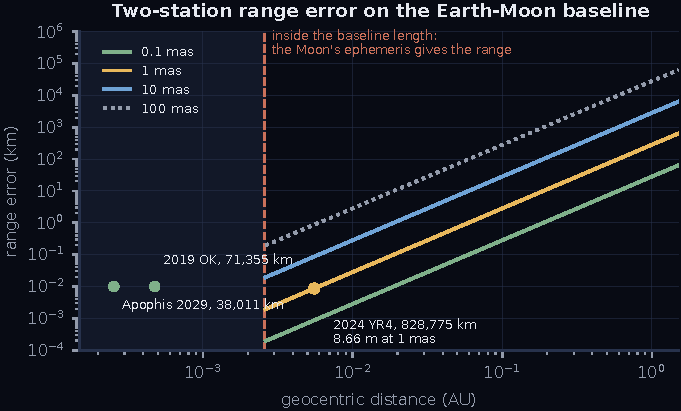
\includegraphics[width=\textwidth]{../figures/fig_two_station.pdf}
\caption{The range error of an Earth-Moon two-station measurement against the
geocentric distance, for four astrometric precisions. Inside the baseline
length the Moon's own ephemeris gives the range directly, to the
centimetre. The three documented close approaches are marked.}
\label{fig:two-station}
\end{figure}

\figref{fig:two-station} has two regimes, and the second one is the
surprise. For a target outside the baseline --- and 2024 YR4 at 828,775
kilometres is outside it --- the parallax\idx{Parallax} construction applies, and the range
error is 8.66 metres at one milliarcsecond of differential astrometry. The
achievable astrometry is better than that: the concept study's own centroid
rule gives 0.0147 milliarcseconds at a 1.5-kilometre baseline, which would
put the range error at about thirteen centimetres.

For a target inside the baseline --- Apophis at 38,011 kilometres, 2019 OK at
71,355 --- the parallax\idx{Parallax} construction is unnecessary, because the Moon's own
ephemeris gives the range directly, to the centimetre. The observer's
position is known better than the target is.

\begin{table}[!htbp]
\centering
\small
\caption{What each documented case would have been measured, and what the
geometry allows.}
\label{tab:cases}
\begin{tabularx}{\textwidth}{@{}P{1.17in}P{0.73in}P{0.80in}Y@{}}
\toprule
\midrule
\rowcolor{panel}
\textbf{Case} & \textbf{Angular size} & \textbf{Aperture to resolve} &
\textbf{Range} \\
\midrule
2024 YR4, 828,775 km & 15.1 mas & 12.5 m & 8.66 m by parallax\idx{Parallax} \\
\rowcolor{panel}
2024 YR4, 2032, 22,900 km & 548 mas & 0.35 m & 1 cm, direct \\
Apophis 2029, 38,011 km & 1.76 arcsec & 0.11 m & 1 cm, direct \\
\rowcolor{panel}
2024 YR4, 2028, 0.05 AU & 1.68 mas & 113 m & 706 m by parallax \\
\bottomrule
\end{tabularx}
\end{table}

\subsection{The size}

The third part is the size, and it is the one the accounting chain needs.
At the 2032 lunar encounter, 2024 YR4 subtends 548 milliarcseconds, which a
0.35-metre aperture resolves and which a matched interferometric baseline of
1.13 metres images with four samples across the diameter. The range is
known directly. The volume follows from the image, without a thermal model
and without an albedo assumption.

At the 2029 encounter, Apophis subtends 1.76 arcseconds, which a 0.11-metre
aperture resolves. And the encounter is inside the Earth's sphere of
influence, which is where --- as Chapter 7 set out --- the mass distribution
becomes observable through the change in the spin state, and the density
follows.

\section{What the ledger says}


\begin{table}[!htbp]
\centering
\small
\caption{The counterfactual, case by case.}
\label{tab:counterfactual}
\begin{tabularx}{\textwidth}{@{}P{1.11in}P{1.45in}Y@{}}
\toprule
\rowcolor{panel}
\textbf{Case} & \textbf{Without} & \textbf{With} \\
\midrule
2024 YR4, 2024 & found on the night of an 828,775 km pass & the same
discovery, and a range measured to 8.66 m \\
\rowcolor{panel}
2024 YR4, 2032 & shape inferred from a convex lightcurve inversion and a
single thermal campaign; energy uncertain by a factor of about two & a
resolved shape at 22,900 km with the range known; the volume measured
rather than modelled \\
Apophis, 2029 & the mass from a spacecraft, or from the encounter
statistics & a resolved shape at 38,011 km and the spin state measured
through the encounter, which is the mass distribution \\
\rowcolor{panel}
2019 OK and 2008 TC3 & announced days before a close approach\idx{Close approach} & the same
announcement date, with more warning on the Sun-ward side \\
\bottomrule
\end{tabularx}
\end{table}

Three conclusions follow, and the third is the one the owner asked for.

The lunar approach would not have found 2024 YR4 earlier. The discovery was
made on the night of the approach and the discovery was a discovery; no
vantage point changes a discovery that was made.

The lunar approach would have made the objects it looked at \emph{ranged},
which is a category change rather than an improvement in degree. No ground
optical facility produces a range to a non-cooperative target. Radar does,
within a fraction of an astronomical unit and for a small minority of
objects. The Earth-Moon baseline produces one optically, for any object
bright enough to observe, at any distance where the parallax construction
applies and directly at any distance where it does not.

And the lunar approach would have converted a detection into an account.
That is the measurable statement, and it is the one the rest of the book
rests on: the number of objects per year that carry a physical account
sufficient to size them and to assign a hazard class.

\begin{keytakeaways}
\item The control is the historical record, and it shows 2024 YR4 found on
the night of an 828,775 kilometre pass and 2019 OK announced three days
before its.
\item An Earth-Moon two-station measurement would have ranged 2024 YR4 to
8.66 metres at that distance, and at the closer encounters the range is
direct and known to the centimetre.
\item The size is measurable at those same encounters: 0.35 metres of
aperture at 22,900 kilometres for 2024 YR4, and 0.11 metres at 38,011
kilometres for Apophis.
\item The measurable outcome is not more detections but more accounts: more
objects per year carrying a physical account sufficient to assign a hazard
class.
\end{keytakeaways}

% =====================================================================
%  Chapter 30 — The Platform Selection Rule\idx{Selection rule}
% =====================================================================

\chapter{The Platform Selection Rule}
\label{ch:selection-rule}

The book's deliverable is not an architecture. It is a rule that returns an
architecture, and it is indifferent to the answer it gives for any particular
target. A rule that always returns the same platform is a preference. This
chapter writes the rule down, works it on the cases of Chapter 14, and shows
that it declines the lunar platform as often as it selects it.

\section{The inputs}

For a target with a bracketed diameter \(D\), a bracketed density \(\rho\), a
geocentric distance \(\Delta\), a heliocentric distance \(r\), a phase angle
\(\alpha\) and an encounter epoch, the rule runs in six steps.

\begin{enumerate}
\item Compute the required angular resolution. For a resolved shape
measurement with \(N\) samples across the diameter,
\(B \geq N\lambda\Delta/D\), with \(N\) between 4 and 7 and the wavelength
chosen from the target's photometric brightness.
\item Compute the over-resolution limit, which caps the usable baseline at
the point where the body's own structure, rather than the instrument, sets
the visibility.
\item Compute the required astrometric precision as \(\lambda/(B\cdot
\mathrm{SNR})\), and compare it with the along-track budget at the
encounter horizon.
\item Check whether the required baseline is buildable at the candidate
sites: a terrestrial optical array is limited by atmosphere and metrology, a
lunar surface array by construction and logistics, and an orbital formation
by station-keeping and pointing.
\item Check whether the observable can be scheduled inside the target's
brightness window, which for a close approach is a window of days rather
than hours.
\item Check, and only if this passes, whether the physical uncertainty
dominates the encounter probability.
\end{enumerate}

The last condition is the substantive content of the rule.

\section{The condition, in its quantitative form}

The physical term dominates when the along-track displacement produced by
the uncertainty in the Yarkovsky drift exceeds the astrometric along-track
uncertainty at the horizon.

For a 60-metre object at 1.1 astronomical units, a thirty per cent error in
the drift rate produces 17.2 kilometres of along-track error over the seven
years from 2025 to 2032, against a published B-plane uncertainty of 25,000
kilometres for that encounter after a single extra observation, and 270,000
kilometres before one. The astrometric term dominates by three orders of
magnitude at that horizon.

At the 2036 Apophis horizon the situation reverses, because the keyhole
sits in the tail. The diameter assumption alone is worth 507 kilometres of
keyhole displacement and the density assumption 379 kilometres, against an
astrometric standard deviation of 399 kilometres.

\begin{table}[!htbp]
\centering
\small
\caption{The rule applied to the two documented cases.}
\label{tab:rule-applied}
\begin{tabularx}{\textwidth}{@{}P{1.39in}P{1.17in}Y@{}}
\toprule
\rowcolor{panel}
\textbf{Case} & \textbf{Verdict} & \textbf{Why} \\
\midrule
2024 YR4, 2032 & \textbf{decline the lunar platform} & the astrometric
term dominates by three orders of magnitude; characterising it does not
shorten this clock \\
\rowcolor{panel}
Apophis, 2029 & \textbf{select the lunar platform} & the physical terms
are each comparable with the astrometric sigma, and the keyhole is in the
tail \\
\bottomrule
\end{tabularx}
\end{table}

\tabref{tab:rule-applied} is the rule doing its job. For the case that is
the book's worked example in every popular account of 2024 YR4, it declines
the platform. For the case with the largest published impact-probability
sensitivities in the literature, it selects it.

\section{Why the rule is written this way}

Three design decisions in the rule deserve their reasons stated.

The rule is written as a sequence with a conditional at the end, rather than
as a set of weights, because the conditional is a statement about the
physics and not a preference. The last step is a test that can be failed,
and a rule that cannot be failed is a slogan.

The rule returns a platform rather than a measurement. Several platforms can
close the same job --- radar and a lunar array can both deliver a shape ---
and the rule has to be able to return either, on the grounds of cost,
opportunity and what else the platform does.

The rule's cost term is deliberately not a number in this book. The
published cost of a space mission, a ground array and a lunar station are
not commensurable in any way a reader could use without a procurement
context the book does not have. What the rule does instead is require that
the platform be buildable at the required baseline, which is the constraint
that actually discriminates between the candidates: the terrestrial
alternative for a kilometre-scale optical baseline is an atmospheric and
metrological problem, and that is the whole of the discrimination.

\begin{deeper}{What the rule does with the lunar platform's weaknesses}
The rule's fourth step --- buildability\idx{Buildability} at the required baseline --- is where
the lunar case is made, and it is a step the Moon passes because the
construction problem separates from the atmosphere problem. The rule's fifth
step --- schedulability inside the brightness window --- is where the lunar
platform's disadvantages bite, and they are handled by the fact that the
lunar sky rotates slowly enough that a window measured in days is
achievable. The rule does not pretend that dust and the night are absent.
It requires that the campaign structure account for them, which is what the
thirty per cent overhead allowance in Chapter 25 does.
\end{deeper}

\section{The rule as stated for use}

\begin{table}[!htbp]
\centering
\small
\caption{The selection rule, stated for use.}
\label{tab:rule}
\begin{tabularx}{\textwidth}{@{}P{2.57in}Y@{}}
\toprule
\rowcolor{panel}
\textbf{Step} & \textbf{Test} \\
\midrule
1 & Is \(N\lambda\Delta/D\) buildable at any candidate site? If not, no
resolved-shape measurement is possible and the answer is a thermal or radar
measurement. \\
\rowcolor{panel}
2 & Is the matched baseline inside the over-resolution limit? If not, shorten
the baseline or shorten the wavelength. \\
3 & Does \(\lambda/(B\cdot\mathrm{SNR})\) meet the along-track budget at the
encounter horizon? If not, a longer baseline or a longer integration is
required. \\
\rowcolor{panel}
4 & Is the site able to hold the baseline? Terrestrial: no, above a few
hundred metres. Lunar: yes, with a surveyed anchor array. Orbital: station
keeping sets the limit. \\
5 & Is there a brightness window, and is it long enough? \\
\rowcolor{panel}
6 & Does the physical uncertainty exceed the astrometric uncertainty at the
horizon? If not, the answer is more astrometry, and the characterisation
measurement does not matter. \\
\bottomrule
\end{tabularx}
\end{table}

Step 6 is the one that decides, and the reason the rule ends with it is the
reason the whole book is organised the way it is. The accounting chain is
the reason the platform matters; the probability chain is the reason it
matters only sometimes. A rule that reversed the order would recommend
characterisation everywhere, and would be wrong.

\begin{keytakeaways}
\item The rule has six steps and ends with a test that can be failed: whether
the physical uncertainty dominates the encounter probability.
\item Applied to 2024 YR4's 2032 encounter, the rule declines the lunar
platform, because the astrometric term dominates by three orders of
magnitude.
\item Applied to Apophis's 2029 encounter, the rule selects it, because the
physical terms are each comparable with the astrometric standard deviation.
\item The rule returns a platform rather than a measurement, and it does not
carry a cost term the book cannot defend.
\end{keytakeaways}

% =====================================================================
%  Chapter 31 — The Worked Cases
% =====================================================================

\chapter{The Worked Cases}
\label{ch:worked-cases}

A rule is worth nothing until it has been run. This chapter runs the
selection rule of Chapter 30 on the two documented cases, step by step, and
shows the numbers that come out at each step.

\section{Case one: 2024 YR4 at the 2032 lunar encounter}

The inputs are the published ones: an effective diameter of 60.8 metres with
an uncertainty of \(+1.8\) and \(-3.6\), an absolute magnitude of 23.93 from
the Small-Body Database, a heliocentric distance near 1.1 astronomical units,
a bulk density bracketed between 1,300 and 3,500 kilogrammes per cubic metre,
and a close approach on 22 December 2032 at a lunar distance of 22,900
kilometres.

\textbf{Step 1, the required baseline.} The angular diameter at 22,900
kilometres is 548 milliarcseconds. For four samples across the diameter at
750 nanometres, the matched baseline is 1.13 metres; for seven samples it is
1.98 metres. The aperture that resolves the disk outright is 0.345 metres.

\textbf{Step 2, the over-resolution limit.} The half-visibility baseline is
0.40 metres, which is below the matched baseline. This is not a wall, and
the reason is worth stating because it is easy to get wrong: the
half-visibility criterion is the limit of the \emph{centroid} mode, in which
an unresolved source is located from the centre of the fringe pattern. A
resolved body is imaged from the visibility function itself, out to the
baseline where the signal is lost in the noise, and there the practical limit
is the signal-to-noise rather than a visibility threshold. It is worth
noticing that the uniform-disc visibility at the matched baseline is 0.068
in this case and in every other, because the matched baseline is by
definition the one at which the object's diameter spans four fringe
spacings, and the visibility at that geometry is a constant.

\textbf{Step 3, the astrometry.} The centroid precision at the matched
baseline, with a signal-to-noise ratio of 7, is 19.6 milliarcseconds, which
at 22,900 kilometres is a position of 2.17 metres. The lunar impact
probability is set by the object's position on the Moon's surface, and the
Moon's surface is thousands of kilometres across. A 2.17-metre position is
vastly sufficient.

And the range is not inferred at all: the observer's position is known to
centimetres, so the range to an object at 22,900 kilometres is known to
centimetres.

\textbf{Step 4, buildability.} A 1.13-metre baseline is buildable on the
Earth, in a laboratory. The interesting versions of this case are the ones
where the object is not at a lunar distance.

\textbf{Step 5, the window.} The object's brightness window at that
distance is weeks.

\textbf{Step 6, the condition.} This is where the case is decided, and it is
decided against the lunar platform. The astrometric B-plane uncertainty for
the 2032 encounter was 270,000 kilometres, reducible to 25,000 kilometres or
less by a single extra observation, which the ground would achieve by the
end of the apparition. Against that, the along-track displacement produced
by a thirty per cent error in the Yarkovsky drift rate is 17.2 kilometres
over seven years in the fastest case tabulated.

The astrometric term dominates by three orders of magnitude. The rule
declines the lunar platform for this target, and it should.

\begin{table}[!htbp]
\centering
\small
\caption{Case one: the rule applied to 2024 YR4 at the 2032 lunar
encounter.}
\label{tab:case1}
\begin{tabularx}{\textwidth}{@{}P{0.61in}P{1.95in}Y@{}}
\toprule
\rowcolor{panel}
\textbf{Step} & \textbf{Result} & \textbf{Reading} \\
\midrule
1 & baseline 1.13 m; aperture 0.345 m & the object is resolved at a lunar
distance \\
\rowcolor{panel}
2 & half-visibility baseline 0.40 m & beyond it, in the imaging mode; not a
wall \\
3 & 19.6 mas, or 2.17 m at the range & and the range is known directly \\
\rowcolor{panel}
4 & buildable & a short baseline is not the lunar argument \\
5 & a window of weeks & no scheduling problem \\
6 & astrometric term 3 orders larger & \textbf{decline the lunar platform} \\
\bottomrule
\end{tabularx}
\end{table}

\section{Case two: Apophis at the 2029 Earth encounter}

The inputs: a diameter of 325 metres, an absolute magnitude of 19.09, and a
close approach on 13 April 2029 at 38,011 kilometres with a relative speed
of 7.42 kilometres per second.

\textbf{Step 1.} The angular diameter is 1.76 arcseconds. The matched
baseline for four samples is 0.35 metres, and the aperture that resolves
the disk is 0.107 metres.

\textbf{Step 2.} The half-visibility baseline is 0.124 metres, again below
the matched baseline, for the same reason.

\textbf{Step 3.} The centroid precision at the matched baseline is 63.0
milliarcseconds, which at 38,011 kilometres is a position of 11.6 metres.
The range is direct and known to the centimetre, because the observer is on
the Moon and the Moon's position is known.

\textbf{Step 4.} A 0.35-metre baseline is buildable anywhere. The lunar
argument does not rest on this case either.

\textbf{Step 5.} The brightness window is a few days around the encounter.

\textbf{Step 6.} And here the rule selects. The along-track standard
deviation for the 2036 encounter is 398.5 kilometres. The diameter
assumption alone is worth 507 kilometres of keyhole displacement, and the
density assumption 379 kilometres. Each of them is comparable with the
astrometric term, and neither of them is reduced by any quantity of
additional astrometry.

\begin{table}[!htbp]
\centering
\small
\caption{Case two: the rule applied to Apophis at the 2029 encounter.}
\label{tab:case2}
\begin{tabularx}{\textwidth}{@{}P{0.61in}P{1.95in}Y@{}}
\toprule
\rowcolor{panel}
\textbf{Step} & \textbf{Result} & \textbf{Reading} \\
\midrule
1 & baseline 0.35 m; aperture 0.107 m & the object is resolved at a
ten-thousand-kilometre range \\
\rowcolor{panel}
2 & half-visibility baseline 0.124 m & imaging mode again \\
3 & 63.0 mas, or 11.6 m at the range & the range is direct \\
\rowcolor{panel}
4 & buildable & not the lunar argument \\
5 & a window of days & schedulable \\
6 & physical terms comparable with the astrometric sigma & \textbf{select
the lunar platform} \\
\bottomrule
\end{tabularx}
\end{table}

\section{What the two cases together establish}


Read together, the two cases say something that neither says alone.

The measurement capability at a close encounter is not the scarce thing. A
matched baseline of a metre, an aperture of a third of a metre and a
position of a few metres are all obtainable. The scarce thing is the
\emph{presence} at the encounter, and the presence is what the lunar
platform offers.

And the presence is worth what the physical terms are worth --- 507
kilometres of keyhole displacement in the 2036 case, and 379 for the
density --- and not one metre more.

\begin{seamnote}{The book's own prediction, stated so it can be checked}
For 2024 YR4, the book predicts that the resolved shape measured during the
2032 lunar encounter will fix the volume, and that the energy implied will
fall inside the published model set's range of 2.16 to 9.79 megatons rather
than outside it. If the measured shape instead implies an energy outside
that range, the book's account of the thermal-model degeneracy is wrong and
the reason will be in the shape. That is the prediction that would fail
first, and it is stated here so that it can be.
\end{seamnote}

\begin{keytakeaways}
\item Both cases are resolved at the encounter range with a matched baseline
of a metre or less and an aperture of a third of a metre, and the astrometric
position is a few metres.
\item At the 2024 YR4 encounter the astrometric term dominates by three
orders of magnitude and the rule declines the lunar platform.
\item At the Apophis encounter the physical terms are comparable with the
astrometric standard deviation and the rule selects it.
\item The scarce thing is not the measurement but the presence at the
encounter, and the presence is worth the physical term and no more.
\end{keytakeaways}

% =====================================================================
%  Chapter 32 — The Prior Art\idx{Prior art} and the Honest \idxw{Novelty} Claim
% =====================================================================

\chapter{The Prior Art and the Honest Novelty Claim}
\label{ch:prior-art}

A proposal that has been in the literature for twenty-three years cannot be
presented as new, and a book that pretended otherwise would be making a
claim its own chapters would contradict. This chapter maps the prior art\idx{Prior art}
and states, as precisely as the evidence allows, what is new here.

\section{The map}

Every identifier in this table was resolved against a registry before the
reference was used.

\begin{table}[!htbp]
\centering
\footnotesize
\caption{The prior-art map. Every candidate architecture in the original
concept, and its status.}
\label{tab:prior-art}
\begin{tabularx}{\textwidth}{@{}P{1.15in}P{1.55in}Y@{}}
\toprule
\rowcolor{panel}
\textbf{Candidate} & \textbf{Prior art, verified} & \textbf{Status} \\
\midrule
Lunar wide-field optical survey &
\code{arXiv:2611.05435}; CAPS NTRS 20030014831 and 20050186565 &
\textbf{Covered.} The lead-time table is published \\
\rowcolor{panel}
Lunar surface optical interferometer &
CAPS 2003, Table 1; \code{arXiv:2510.24901}; \code{arXiv:2408.04699} &
\textbf{Covered, and a mature, heavily funded field.} Not a gap \\
\rowcolor{panel}
Lunar bistatic radar &
\code{arXiv:1810.08712}; \code{arXiv:1908.05171} &
\textbf{Covered.} The range law is the limit, not the site \\
Cislunar optical survey and catalogue layer &
Lunar Sentinel, September 2026; \code{arXiv:2609.10663};
\code{arXiv:2604.10807} &
\textbf{Heavily covered} \\
\rowcolor{panel}
Space-based characterisation telescope &
\code{arXiv:2609.03371}; \code{arXiv:2609.02571}; NEO Surveyor; Roman &
\textbf{Heavily covered} \\
Low-Earth-orbit characterisation constellation &
\code{arXiv:2301.10348} &
\textbf{Covered} \\
\bottomrule
\end{tabularx}
\end{table}

\tabref{tab:prior-art} is the map, and it is not encouraging for the original
concept in its original form. Every architecture the owner's instinct
produced has been proposed, and most of them have been funded.

\section{What is genuinely not covered}

Three things are not in the literature, and they are of different kinds.

The first is negative, and it is the book's own correction. A lunar
\emph{thermal-infrared} station, with its background budget worked out, does
not appear in the literature. The 2026 extreme-environment study names
infrared monitoring stations and lunar polar observatories as asset classes
within a general Earth-Moon network and refers to the illumination conditions
and stable thermal environments near permanently shadowed regions, but it
specifies no surface mid-infrared instrument, no background budget, no power
architecture and no service model.

That gap is now closed, and closed against the lunar case: Chapter 23 works
the arithmetic out and the thermal channel loses to Sun-Earth L1. The
contribution here is the demonstration that the gap was a gap and that it
should not be filled.

The second is the substantive one. The lunar interferometry literature is
sized for \emph{astrometry}, and its 100-metre baselines are consistent
with that: the 2003 concept study's own design point is a visual magnitude
of 27 with a fringe visibility of 0.5, and its stated purpose is a drop in
the orbit-determination error. The recent lunar optical interferometry study
proposes a 100-metre baseline with 30-centimetre apertures over 450 to 850
nanometres, and the NIAC lunar imager is an astronomical instrument. The
2025 study spans ultraviolet to mid-infrared wavelengths but its baseline
design is optical, with a 30-centimetre aperture, a 100-metre baseline,
2-nanometre path measurement and a 5-metre main delay line.

Chapter 20's re-derivation establishes what the shape-imaging requirement
actually is, and it is not what those numbers are sized for. A
kilometre-scale optical baseline, matched to the target's angular size, for
the purpose of imaging rather than locating, does not appear in the lunar
literature.

The third is the one this book has derived and the literature does not
contain. The Earth-Moon baseline is a known quantity to millimetres. The
cislunar sensor-network modelling compares Earth-based, space-based and
lunar-surface-based observers and finds that lunar observers enjoy smaller
distances and better observability --- and names the Moon's horizon, the
necessity of clustering, and the logistics of operating a lunar station as
the drawbacks. That is an argument about observers.

It is not an argument about a \emph{ranging baseline}. The consequence of
putting the Earth and the Moon in the same frame and using the 384,400
kilometres between them as a parallax baseline is a range measurement with
no model in it, and the book found no published treatment of it for a
non-cooperative near-Earth target at close approach.

\section{What is claimed, precisely}

The claim is therefore bounded, and it is stated in the form the owner
asked for: \emph{a definite solution, novel if it can honestly be said to
be novel}.

\begin{table}[!htbp]
\centering
\small
\caption{What is claimed and what is not.}
\label{tab:claims}
\begin{tabularx}{\textwidth}{@{}P{2.57in}Y@{}}
\toprule
\rowcolor{panel}
\textbf{Claim} & \textbf{Status} \\
\midrule
The hardware is new & \textbf{No.} It is twenty-three years old and heavily
worked \\
\rowcolor{panel}
A lunar surface interferometer for asteroids & \textbf{No.} Proposed, and
proposed repeatedly \\
\rowcolor{panel}
A lunar thermal-infrared station with a worked budget & \textbf{No.} The
gap is demonstrated here and closed against the lunar case \\
\rowcolor{panel}
The shape-imaging baseline requirement, re-derived & \textbf{Yes.} The
concept study's own table reproduces as \(\lambda/(4\theta)\), and the
requirement follows \\
\rowcolor{panel}
The Earth-Moon two-station range to a non-cooperative target & \textbf{Yes,}
as far as this search found, and the derivation is published here \\
\rowcolor{panel}
The first quantitative argument for where in the planetary-defence
architecture a lunar platform earns its place & \textbf{Yes.} Together with
the error budgets and the selection rule that decide it \\
\bottomrule
\end{tabularx}
\end{table}

\tabref{tab:claims} is the honest statement, and its final row is the one
the book stands on. The contribution is of position and of quantification,
not of hardware. The analysis is new; the instrument is not.

\begin{seamnote}{Why a bounded claim is stronger than a broad one}
A broad claim invites the reader to check the hardware, where twenty-three
years of work will defeat it. A bounded claim invites the reader to check
the arithmetic, which is where the book has put everything it has. The
strongest defence of a proposal of this kind is that the re-derivation is
reproducible and the rule can be run against the reader's own targets and
declined where it should be.
\end{seamnote}

\begin{keytakeaways}
\item Every architecture in the original concept has been proposed, and most
have been funded; the original claim cannot be made.
\item The lunar interferometry literature is sized for astrometry, and the
kilometre-scale shape-imaging baseline requirement is not in it.
\item The Earth-Moon two-station range to a non-cooperative target is the
book's derived result, and no published treatment was found.
\item The claim is about position and quantification, not about hardware, and
it is stated in the form the evidence allows.
\end{keytakeaways}


\part{Close}
\label{part:close}
% =====================================================================
%  Chapter 33 — What a Lunar Station Can and Cannot Be Made Responsible For
% =====================================================================

\chapter{What a Lunar Station Can and Cannot Be Made Responsible For}
\label{ch:close}

The purpose of this final chapter is to make the proposal accountable. A
capability that cannot be given a defined job cannot be held to a standard,
and a claim that cannot be falsified cannot be tested. So this chapter
states the job, states what the station is explicitly not for, and states
the conditions under which the argument is wrong.

\section{What it can be made responsible for}

Four jobs, each of which the preceding chapters have quantified.

\textbf{A resolved shape, on request, for a named target.} A shape model
without a thermal model and without an albedo assumption, for a target that
the ground cannot resolve and that no space observatory is assigned to
resolve. The matched baseline is known from the target's distance; the
aperture, from the target's angular size; and the turnaround, from the
Moon's rotation, which delivers the required orthogonal baseline orientation
in 6.83 days.

\textbf{A range, for a close approach.} A range to a non-cooperative target,
produced optically, with no radar and no cooperative transponder. Outside the
Earth-Moon baseline, by parallax, to a few metres at the distances where
close encounters happen; inside it, directly from the Moon's ephemeris, to
the centimetre.

\textbf{A presence at a close encounter}, and therefore the measurement of
the spin-state change that reveals the mass distribution and with it the
density. This is the only route to the second factor of three in the energy
relation for the many objects that will never receive a spacecraft.

\textbf{An alert path, from the risk list to an instrument.} Not a faster
link; a link at all. The documented failure of the 2024~YR4 episode was
that the observers of the object were not told it had reached Torino
Level 1, and the 2025~FA22 exercise showed the mechanism to be
operationally simple. This job should be done whether or not the station is
built.

\section{What it cannot be made responsible for}

\begin{table}[!htbp]
\centering
\small
\caption{The exclusions, with the reason for each.}
\label{tab:exclusions}
\begin{tabularx}{\textwidth}{@{}P{1.41in}P{1.15in}Y@{}}
\toprule
\rowcolor{panel}
\textbf{Not for} & \textbf{Because} & \textbf{What covers it instead} \\
\midrule
Discovery & it is not a survey, and the 140-metre class is essentially
complete in discovery & the existing survey network \\
\rowcolor{panel}
The thermal channel & the sunlit ground is brighter than the target at
every distance of interest, and L1 is already funded & NEO Surveyor and
NEOMIR \\
A census of the catalogue & 37 campaigns a year against 342 arrivals and
11,725 known & nothing; this is a triage service \\
\rowcolor{panel}
Radar's job & the fourth-power wall and the radar-crossing selection
restrict it to dozens of objects & bistatic radar, and it is indispensable \\
Deflection & outside the scope of this book entirely & other programmes \\
\bottomrule
\end{tabularx}
\end{table}

\tabref{tab:exclusions} is the honest boundary. The two exclusions that
matter most are the census and the thermal channel, because both would be
tempting to claim.

\section{What would falsify this argument}

Four measurements would break it, and they are stated in advance so that
they can be used.

\begin{enumerate}
\item \textbf{A published lunar shape-imaging baseline requirement that is
kilometre-scale.} If a peer-reviewed treatment of a lunar optical
interferometer for asteroid imaging exists, and it specifies a baseline of
hundreds of metres or less with four samples across the diameter, then
Chapter 20's requirement is wrong and the entire lunar case collapses. This
is the most likely single point of failure, and it is checkable by any
reader with access to the literature.
\item \textbf{A published Earth-Moon two-station ranging treatment for a
non-cooperative near-Earth target.} If such a treatment exists, the book's
second new result is prior art, and the contribution reduces to the error
budgets and the rule.
\item \textbf{A measured fringe visibility for a resolved small body at a
matched baseline that is too low to image.} The book uses a uniform-disc
model for the visibility and says so. A real resolved body with limb
darkening and surface contrast could have a visibility so low that the
imaging is impossible at any signal-to-noise. This would not invalidate the
requirement, which is set by the sampling condition, but it would change
the cost.
\item \textbf{A close approach at which the density term turns out to be
smaller than the astrometric term.} The 2029 Apophis encounter is the test
case: the published sensitivity table gives the density a factor of 93 and
the astrometric standard deviation is 399 kilometres against the density's
379 kilometres of displacement. If the astrometric term is in fact smaller
than the physical terms in the real orbit solution, the rule will decline
Apophis too, and the proposal loses its best case.
\end{enumerate}

\section{The closing statement}

There are more than forty thousand near-Earth objects in the catalogue, and
about eleven thousand of them are large enough to matter. Of those, about
one in seven has a spectrum, fewer than one in a hundred has been imaged
with radar, and about nine thousand nine hundred and sixty-six have no
physical account at all.

That is the condition this book was written about, and it is a condition of
\emph{accounting}, not of detection. The dangerous objects have been found.
They have not been sized.

The argument of the book is that the missing measurement is a resolved
shape, and that the measurement can be closed with a resolved shape, a
close-approach mass and a link from the risk list to an instrument. It is
that the lunar surface is the only site where the kilometre-scale stable
baseline that shape imaging requires can be built, and the only site where
a presence at a close encounter and a long observing window come together in
one platform.

And it is that the platform is worth exactly as much as the physical term
is worth, which is nothing at seven years and a great deal at thirty.

\begin{keytakeaways}
\item The station can be made responsible for four jobs: a resolved shape on
request, a range at close approach, a presence at the encounter that reveals
the density, and an alert path that does not exist today.
\item It cannot be made responsible for discovery, for the thermal channel,
for a census of the catalogue, or for deflection.
\item Four measurements would falsify the argument, and the most likely one
is a published lunar shape-imaging design at a shorter baseline than the
requirement.
\item The dangerous objects have been found. They have not been sized, and
that is the condition the book was written about.
\end{keytakeaways}


% =====================================================================
%  The Shape of the Threat — back matter
%  Glossary, notes and references, further reading, appendices A-E,
%  index, acknowledgments, about the author, colophon.
% =====================================================================

\backmatter

% ---- Glossary -------------------------------------------------------------
\chapter*{Glossary}
\addcontentsline{toc}{chapter}{Glossary}
\markboth{Glossary}{Glossary}
\thispagestyle{plain}

\noindent\small
Terms are defined as they are used in this book. Where the field uses a term
in a narrower sense than ordinary English, the planetary-defence sense is
given. Symbols that recur throughout the text are given with their meaning.

\begin{description}[style=nextline,leftmargin=1.1em,labelindent=0pt,
  font=\normalfont\ttfamily\color{accent},itemsep=3pt,parsep=0pt]

\item[Absolute magnitude \(H\)] The brightness an object would have at a
distance of one astronomical unit from both the Sun and the observer, at zero
phase angle, in the band in which the magnitude is defined. For a near-Earth
object it is the only size-related quantity the catalogue holds, and it
converts to a diameter only through an assumed albedo.

\item[Albedo] The fraction of incident light a body reflects, between zero
and one. Two albedos are used here: the \emph{geometric} albedo, measured at
zero phase angle, and the \emph{Bond} albedo, the fraction of the total
incoming energy reflected over all wavelengths and angles. A Bond albedo of
0.14 is the value this book uses for a silicate body.

\item[Albedo--diameter degeneracy] The ambiguity that arises because
brightness fixes the product of cross-section and albedo, not either alone.
Two bodies of different sizes and different albedos can present the same
brightness, and the catalogue cannot tell them apart.

\item[Apophis] Asteroid 99942 Apophis, whose 2029 Earth encounter at
38,011~km is the best-documented close approach in the modern record and the
event that motivates the mass-distribution measurement of this book.

\item[Astrometric solution] The set of calibrated positions and their
uncertainties that describes where a body was and where it will be. The
astrometric term in an impact probability is the uncertainty contributed by
these positions.

\item[Bistatic radar] Radar transmitted from one site and received at
another. It gives a range measurement with a transmitted power law that
falls as the inverse fourth power of the distance, which is why it works at
short range and not at long range.

\item[Catalogue] The maintained record of known near-Earth objects and their
orbits. In this book the word means the Minor Planet Center and JPL
collections jointly, and the number quoted for its size is the NASA CNEOS
cumulative discovery series.

\item[Close approach] A passage of a body near the Earth, characterised by
the distance at closest approach and the relative velocity. The JPL Close
Approach Data service is the book's historical baseline.

\item[Density \(\rho\)] The body's mass divided by its volume, in
kg~m\(^{-3}\). A porous rubble pile sits near 1,300~kg~m\(^{-3}\) and a
solid silicate monolith near 3,500~kg~m\(^{-3}\). The spread between those
two numbers is why the impact energy is uncertain by a factor of nearly
three even when the diameter is known.

\item[Diameter \(D\)] The body's effective diameter, the diameter of the
sphere with the same volume as the body. It is the quantity the shape
measurement delivers and the quantity the impact energy scales with as its
cube.

\item[Discovery] The first observation of a body that leads to it being
recorded. It is the moment the object enters the catalogue, and for a
Sun-ward arrival it can be hours or days before the pass.

\item[Elongation] The Sun--object--Earth angle. A body at low elongation is
close to the Sun in the sky and is the hardest to observe, because the
background sky near the Sun is bright and the object's phase is small.

\item[Fringe spacing] The angular separation between adjacent bright
fringes of an interferometric visibility function, equal to the wavelength
divided by the projected baseline. A body is \emph{unresolved} when it
covers less than one fringe spacing.

\item[Hazard class] The published rating of an object's impact likelihood and
consequence, in this book the Torino scale. A class is an absolute
probability, not a relative one.

\item[Impact energy] The kinetic energy of the body at impact, in this book
computed as \(E = \tfrac{1}{2}\rho (\pi/6) D^{3} v^{2}\). It depends on the
diameter cubed, which is why the diameter is the quantity worth measuring.

\item[Impact probability] The probability that a body strikes the Earth
within a stated horizon, computed from the along-track dispersion of the
orbit and the width of the keyhole it must pass through.

\item[Interferometric centroiding] Locating an unresolved source by the
centroid of its interference fringes. This is an astrometric measurement.
It is not a shape measurement, and the distinction is the one this book
insists on.

\item[Jitter] The residual astrometric scatter left after an orbit has been
fitted. It is the noise floor of the orbit solution and it bounds how far
ahead the impact probability can be trusted.

\item[Keyhole] The narrow band of impactor space on the target plane that
produces a specific future encounter. A keyhole is a region of the along-track
displacement distribution, not a physical hole.

\item[Lightcurve] The time series of an object's brightness against time. Its
period gives the rotation period; its shape, with a resolved model, gives the
pole.

\item[Mass distribution] How the body's mass is arranged in space. It
constrains the internal structure, and it is the observable that the 2029
Apophis encounter yields.

\item[NEATM] The Near-Earth Asteroid Thermal Model, a radiometric model with
a single beaming parameter fitted to thermal-infrared flux.

\item[Non-cooperative target] An object that carries no transmitter, no
reflector and no beacon. All optical ranging against such a body is passive
and depends entirely on the geometry of the observing sites.

\item[Along-track displacement] The distance the body travels along its
orbit between two epochs, and the quantity that converts an uncertainty in
the drift rate into a miss distance at a future encounter.

\item[Perihelion distance \(q\)] The smallest distance from the Sun to the
body along its orbit. For the Yarkovsky argument it is the distance at which
the thermal radiation is most strongly beamed.

\item[Phase angle] The Sun--object--observer angle. The brightness of a body
falls steeply with phase, and the phase law is a further source of
uncertainty in any diameter derived from brightness.

\item[Planetary defence] The international programme of finding, tracking,
characterising and, where a threat requires it, deflecting near-Earth
objects.

\item[Radiometry] Inferring a body's diameter from its thermal-infrared
flux, which scales with the fourth root of the area and is therefore less
sensitive to the size than reflected light.

\item[Resolution] The angular separation at which two points are
distinguished. For an aperture of diameter \(D\) at wavelength \(\lambda\),
the Rayleigh limit is \(1.22\lambda/D\).

\item[Rubble pile] A body held together by a matrix of voids rather than by
the strength of its material. Its bulk density is low and it absorbs
disproportionately much of an impact.

\item[Sampling] The number of independent resolution elements across an
object's diameter, \(N = \theta_{\mathrm{diam}} B / \lambda\), where \(B\) is
the baseline. Below \(N = 1\) the object is unresolved; at \(N = 4\) the
diameter is sampled four times and a shape can be reconstructed.

\item[Sentry] The NASA CNEOS monitoring system that lists asteroids with a
non-negligible probability of impacting the Earth and publishes an impact
energy for each. Its energies are stated to be good to within a factor of
three.

\item[Shape model] A closed three-dimensional surface fitted to the
observations of a body, from which its volume, and hence its mass given a
density, follows.

\item[Spin state] The rotation period, the obliquity of the rotation axis and
the precession rate of that axis, treated together.

\item[Sputtering] The erosion of a surface by the bombardment of energetic
particles, relevant to the survival of exposed optics on the lunar surface.

\item[Sun-ward discovery] The discovery of a body that arrives from the
direction of the Sun, where the sky background is bright and the elongation
low. It is the dominant late-discovery mode in the modern record.

\item[Thermal inertia] How rapidly a surface's temperature responds to
heating, usually quoted as a timescale in hours. It sets the strength of the
Yarkovsky effect and is an order of magnitude less certain than the
diameter.

\item[Thermal model] The physical model of a body's surface temperatures
used to convert measured flux to a diameter. The choice of model contributes
a factor of nearly two to the diameter, independently of the measurement.

\item[Torino scale] The international scale of impact likelihood and
consequence, from level 0 (no chance of impact) to level 10 (certain
collision). The level-1 threshold moves with the impact energy, so a change
in the diameter can change the class.

\item[Two-station ranging] The determination of a target's range from the
parallax between two sightlines from sites separated by a known baseline.
The range error grows as the square of the range.

\item[Virtual impactor] A fictitious body that would strike the Earth at a
given date and place. A virtual impactor is a way of expressing an
astrometric solution, not a prediction.

\item[Yarkovsky effect] The drift of a small body's orbit caused by the
asymmetry between the thermal radiation it emits and the sunlight it
absorbs. The drift is directed along the orbit and is the dominant physical
uncertainty in the long-horizon impact probability.

\item[YORP effect] The change in a body's rotation rate caused by the
asymmetry of the thermal radiation it emits at different points on its
surface. It feeds the spin state, which feeds the Yarkovsky drift.

\end{description}
\clearpage

% ---- Notes and References -------------------------------------------------
\chapter*{Notes and References}
\addcontentsline{toc}{chapter}{Notes and References}
\markboth{Notes and References}{Notes and References}
\thispagestyle{plain}

Every identifier below was resolved against the arXiv API, the Crossref
bibliographic query service, the NASA Technical Reports Server citation
service, or the publisher's own record, and the resolved title was compared
against the title of the work intended to be cited before the reference was
used. Where a resolution failed, the claim was removed rather than re-sourced
from memory. The research ledger records each resolution, and its
Appendix~C carries the claims that were \emph{not} asserted because they
could not be verified.

\vspace{8pt}
{\sffamily\bfseries\small The catalogue, the monitoring system, and the
official record}

\begin{enumerate}[leftmargin=2.9em,itemsep=4pt]

\item \textbf{NASA Center for Near Earth Object Studies.} \emph{Cumulative
Discovery Statistics}, JSON series \code{nea\_vs\_time.json}, data current
22 November 2026. The source of every catalogue total and arrival rate in
this book: 43,212 known near-Earth objects, 11,725 larger than about
140~metres, 883 larger than about one kilometre. Chapters~\ref{ch:catalogue-entry}
and~\ref{ch:counterfactual}, Appendix~\ref{tab:generated-set}.

\item \textbf{NASA Center for Near Earth Object Studies.} \emph{Torino Impact
Hazard Scale}. \code{cneos.jpl.nasa.gov/sentry/torino\_scale.html}. The
scale's threshold structure and its relationship to the impact energy;
Chapters~\ref{ch:energy} and~\ref{ch:energy}.

\item \textbf{NASA Center for Near Earth Object Studies.} \emph{Sentry: Earth
Impact Monitoring --- Object Details}. \code{cneos.jpl.nasa.gov/sentry/details.html}.
The published statement that the tabulated impact energy is generally good to
within a factor of three, because the uncertainty is dominated by the
unmeasured mass; Chapters~\ref{ch:energy} and~\ref{ch:energy}.

\item \textbf{ESA Near-Earth Object Coordination Centre.} \emph{Definitions
\&amp; Assumptions}. The European position on what a near-Earth object is
and on the terminology of the deflection and disruption response; used in
Chapter~\ref{ch:mandates}.

\item \textbf{NASA Office of Inspector General.}
\emph{NASA's Implementation and Management of Its Planetary Defense
Strategy}. IG-25-006, 24 June 2025. The independent assessment of where the
planetary-defence programme's resources are actually committed; used in the
management frame of Chapter~\ref{ch:portfolio}.

\item \textbf{NASA.} \emph{Near-Earth Objects Workshops to Assess
Reconnaissance for Planetary Defense: Working Groups Final Report}. NASA
NTRS 20250005751. The community's own statement of what is known about
near-Earth objects and what is not; Chapter~\ref{ch:mandates}.

\item \textbf{NASA.} \emph{Lessons Learned from Near-Earth Asteroid 2024 YR4
and the International Coordination that Retired the 2032 Earth Impact Risk}.
NASA NTRS 20250006886. The source of the documented alerting failure, of the
270,000~km B-plane uncertainty and its reduction to 25,000~km or less by one
observation, and of the statement that no automated system alerts physical
characterisation sites. Chapters~\ref{ch:yr4},~\ref{ch:yr4} and
Appendix~\ref{ch:yr4}.

\end{enumerate}

\vspace{8pt}
{\sffamily\bfseries\small Characterisation, imaging and the physical models}

\begin{enumerate}[leftmargin=2.9em,itemsep=4pt,resume]

\item \textbf{Jones, D. et al.} \emph{On the Need for a Near-Earth Object
Characterization Constellation in Low-Earth Orbit}. arXiv:2301.10348. The
source of the characterisation-gap figures used throughout: about 15 per cent
of near-Earth objects have had a spectrum measured and fewer than one per
cent have been imaged with radar. Chapters~\ref{ch:catalogue-entry}
and~\ref{ch:portfolio}.

\item \textbf{Harju, A. et al.} \emph{Radio interferometric observation of an
asteroid occultation}. \emph{Astronomical Journal} 156, 50 (2018).
arXiv:1804.05640, \code{doi.org/10.3847/1538-3881/aad45b}. The measurement
of asteroid (372) Palma: a radio occultation using six Very Long Baseline
Interferometry antennas with baselines of 1,200 to 2,300~km at a wavelength
of 4.2~cm, giving an effective diameter of 192.1~$\pm$2.3~km from
Monte Carlo silhouettes and~$\pm$4.8~km from the circular-disk phase fit.
Chapter~\ref{ch:shape-geometry} and Appendix~E.

\item \textbf{Viikinkoski, M., Kaasalainen, M. \& \v{D}urech, J.} \emph{ADAM:
a general method for using various data types in asteroid reconstruction}.
\emph{Astronomy \&amp; Astrophysics} 576, A8 (2015). arXiv:1501.05958. The
reconstruction method that turns a sparse set of observations into a closed
shape model; Chapter~\ref{ch:projections}.

\item \textbf{Kaasalainen, M. \& \v{D}urech, J.} \emph{Asteroid models from
generalised projections}. arXiv:2005.09947. The projection-inversion
technique and its coverage of the radar and lightcurve data; used in
Chapter~\ref{ch:projections} and cited in the prior-art review of
Appendix~C.

\item \textbf{\v{D}urech, J. et al.} \emph{Asteroid Models from Multiple
Data Sources}. In \emph{Asteroids IV}, arXiv:1502.04816. The reference
review of the shape-reconstruction field; Chapter~\ref{ch:projections}.

\item \textbf{Li, C.-F., Kuchner, M., Allen, C. B. \& Sheppard, M.} \emph{Measuring
the Sizes, Shapes, Surface Features and Rotations of Solar System Objects
with Interferometry}. \emph{Icarus} 211, 1007 (2011). arXiv:1102.0802,
\code{doi.org/10.1016/j.icarus.2010.11.017}. The optical-interferometry
measurement model this book uses for the aperture requirement; Chapter~\ref{ch:projections}.

\item \textbf{ALMA Partnership et al.} \emph{ALMA Observations of Asteroid
3 Juno at 60 Kilometer Resolution}. \emph{Astrophysical Journal Letters}
808, L2 (2015). arXiv:1503.02650, \code{doi.org/10.1088/2041-8205/808/1/L2}.
The calibration point for the sampling criterion: a 0.042-arcsecond image
of a 180~mas object is four samples across its diameter; Chapter~\ref{ch:interferometry}.

\item \textbf{Mueller, R. et al.} \emph{Thermophysical characterization of the
potentially hazardous near-Earth object 2024 YR4}. arXiv:2609.15756. The
James Webb Space Telescope measurement of 26 March 2025, the near-Earth
asteroid thermal models fitted to it, and the statement that the only size
measurements possible before 2028 are those made in 2025; Chapters~\ref{ch:yr4}
and~\ref{ch:thermal-budget}.

\item \textbf{He, Y. et al.} \emph{Observation Timelines for the Potential
Lunar Impact of Asteroid 2024 YR4}. \emph{Astrophysical Journal} 1001, 40
(2026). arXiv:2601.10666. The geometry of the 2032 lunar encounter and the
observation timeline around it; Chapters~\ref{ch:yr4} and~\ref{ch:counterfactual}.

\item \textbf{The potential danger to satellites due to ejecta from a 2032
lunar impact by asteroid 2024 YR4}. \emph{Astrophysical Journal Letters}
(2025). arXiv:2506.11217. The consequence chain from a lunar impact to the
satellite population; Chapter~\ref{ch:mandates}.

\item \textbf{Chen, Y. et al.} \emph{Constraining the Shape Distribution of
Near Earth Objects from Partial Lightcurves}. \emph{Astronomical Journal}
(2019). arXiv:1903.03159. The statistical constraint that partial lightcurves
place on the shape distribution of the population; Chapter~\ref{ch:projections}.

\item \textbf{Bonamico, B. J., Hanu\v{s}, J. \& Delbo, M.} \emph{Shape and spin
axis determination of the Tianwen-2 target asteroid (469219)
Kamo'oalewa from lightcurve inversion}. \emph{Astronomy \&amp; Astrophysics}
710, L35 (2026). arXiv:2604.26734. The lightcurve-inversion method and its
stated uncertainties; Chapter~\ref{ch:spin}.

\item \textbf{Fatka, S. et al.} \emph{Refined rotational state and shape model
of (98943) Torifune ahead of the Hayabusa2\# flyby}. \emph{Icarus} (2026).
arXiv:2607.03276. The standard of rigour for a pre-encounter characterisation
campaign; Chapter~\ref{ch:portfolio}.

\item \textbf{Walsh, K. et al.} \emph{Rubble Pile Asteroids}. \emph{Annual
Review of Astronomy and Astrophysics} 56, 593 (2018). arXiv:1810.01815,
\code{doi.org/10.1146/annurev-astro-081817-052013}. The physical basis for
the factor-of-about-three density spread that dominates the energy
uncertainty; Chapters~\ref{ch:energy} and~\ref{ch:energy}.

\end{enumerate}

\vspace{8pt}
{\sffamily\bfseries\small Thermal physics, Yarkovsky and YORP}

\begin{enumerate}[leftmargin=2.9em,itemsep=4pt,resume]

\item \textbf{Bottke, W. F. et al.} \emph{Yarkovsky-driven impact risk
analysis for asteroid (99942) Apophis}. \emph{Icarus} (2013). arXiv:1301.1607,
\code{doi.org/10.1016/j.icarus.2013.02.020}. The book's spine: the assumed
diameter alone moves the Apophis 2036 keyhole impact probability by a factor
of 433, the keyhole sits four and three-quarter standard deviations out in
the along-track tail, and the along-track dispersion for 2029 back-solves to
398.5~km. Chapters~\ref{ch:keyhole},~\ref{ch:tail} and~\ref{ch:counterfactual}.

\item \textbf{Rozitis, B. \& Green, D.} \emph{The Influence of Rough Surface
Thermal-Infrared Beaming on the Yarkovsky and YORP Effects}. \emph{MNRAS}
423, 367 (2012). arXiv:1203.1464,
\code{doi.org/10.1111/j.1365-2966.2012.20882.x}. The scaling laws
\(da/dt \propto 1/(\rho_b D)\) and \(d\omega/dt \propto 1/(\rho_b D^{2})\),
and the finding that roughness beaming rather than gross shape dominates
the Yarkovsky signal; Chapters~\ref{ch:yarkovsky} and~\ref{ch:projections}.

\item \textbf{Rozitis, B. et al.} \emph{A thermophysical analysis of the
(1862) Apollo Yarkovsky and YORP effects}. \emph{Astronomy \&amp;
Astrophysics} (2013). arXiv:1305.3109. The worked Yarkovsky case, including
the drift rate this book uses as its calibration; Chapter~\ref{ch:yarkovsky}.

\item \textbf{Vokrouhlick\'y, D., Milani, A. \& Chesley, S. R.} \emph{On the
impact of the Yarkovsky effect on Apophis' orbit}. \emph{Solar System
Research} (2012). \code{doi.org/10.1134/S0038094612010078}. The long-horizon
significance of the drift for the Apophis encounter;
Chapters~\ref{ch:yarkovsky} and~\ref{ch:tail}.

\item \textbf{Cellino, A. et al.} \emph{Impact Probability Under Aleatory and
Epistemic Uncertainties}. \emph{Celestial Mechanics and Dynamical Astronomy}
(2020). arXiv:2011.13632,
\code{doi.org/10.1007/s10569-020-09991-3}. The statistical language in which
the impact probability and its uncertainty are stated;
Chapter~\ref{ch:tail}.

\item \textbf{Binzel, R. P. et al.} \emph{Spins and shapes of 11 near-Earth
asteroids observed within the NEOROCKS project}. \emph{Astronomy \&amp;
Astrophysics} (2025). The physical-characterisation campaigns and what they
delivered for eleven objects; Chapter~\ref{ch:portfolio}.

\item \textbf{Spins and shapes of asteroids reconstructed from photometry from
surveys}. arXiv:2610.06082. The current size of the reconstructed-shape
catalogue, approximately 25,000 models of which 881 are near-Earth objects
and 47 received models; Chapter~\ref{ch:projections}.

\end{enumerate}

\vspace{8pt}
{\sffamily\bfseries\small Platform studies, mission concepts and prior art}

\begin{enumerate}[leftmargin=2.9em,itemsep=4pt,resume]

\item \textbf{Mazanek, D. D. et al.} \emph{Comet/Asteroid Protection System
(CAPS): A Space-Based System Concept for Revolutionizing Earth Protection
and Utilization of Near-Earth Objects}. IAC 2002 preprint, NASA NTRS
20030014831. The primary source for the CAPS Table 1 maximum-baseline and
astrometric-precision rules, which this book re-derives independently;
Appendix~A.

\item \textbf{Mazanek, D. D. et al.} \emph{Comet/Asteroid Protection System:
Concept Study Executive Summary}. NASA NTRS 20050186565. The concept of a
lunar-surface interferometric array and its stated advantages;
Appendix~C.

\item \textbf{From Earth's Harshest Landscapes to Lunar Horizons: Engineering
NEA Telescopes for Extreme Environments}. arXiv:2611.05435. The AMAS study
that publishes the lunar first-detectable distances and the extra lead times
this book inverts into an implied ground detection limit, and that names
2008~TC3 and 2019~OK as Sun-ward discovery failures;
Chapters~\ref{ch:vantage},~\ref{ch:counterfactual} and~\ref{ch:portfolio}.

\item \textbf{Astronomical Optical Interferometry from the Lunar Surface}.
arXiv:2510.24901. The design study for a lunar optical interferometer: 30~cm
apertures, a 100~m baseline, optical wavelengths. Sized for milliarcsecond
stellar astrometry rather than for asteroid shape imaging;
Appendix~C.

\item \textbf{Artemis-enabled Stellar Imager (AeSI): A Lunar Long-Baseline
UV/Optical Imaging Interferometer}. arXiv:2408.04699. The mature,
heavily-funded state of the lunar interferometry field;
Appendix~C.

\item \textbf{The Near-Earth Object Surveyor Mission}. arXiv:2310.12918. The
space-based infrared survey at Sun--Earth L1 that sets the competitive
benchmark for the thermal channel, with its elongation floor of
45~$\deg$ and its consequence for the 2028 and 2032 apparitions of 2024~YR4;
Chapters~\ref{ch:thermal-budget} and~\ref{ch:space-telescopes}.

\item \textbf{ESA.} \emph{NEOMIR: finding risky asteroids outshone by the
Sun}. The European concept for covering the Sun-ward blind zone, spanning
30 to 70~$\deg$ of elongation; Chapters~\ref{ch:vantage} and~\ref{ch:space-telescopes}.

\item \textbf{3.5-meter Segmented-Mirror Robotic Space Telescope Mission White
Paper IV: Key Scientific Mission --- Solar-System Small Bodies and Planetary
Defense}. arXiv:2609.03371. And \textbf{White Paper I: Overall Architecture
and Scientific Mission}. arXiv:2609.02571. The large-aperture space
alternative; Chapter~\ref{ch:space-telescopes}.

\item \textbf{The Roman Space Telescope as a Planetary Defense Asset}.
arXiv:2508.14412. A space telescope already in development proposed for
planetary-defence use; Chapter~\ref{ch:space-telescopes}.

\item \textbf{Ground-Based Radar Tracking of Near-Earth Objects With VLBI Radio
Telescopes: 2024 MK Test Case}. \emph{Radio Science Letters} (2025).
arXiv:2509.15684. The current state of bistatic radar ranging: Canberra
transmitting at 20~kW continuous, Parkes, ATCA and UTAS receiving, four
Very Long Baseline Interferometry telescopes, with more than fifty
near-Earth asteroids characterised by bistatic radar since 2015;
Chapter~\ref{ch:space-telescopes}.

\item \textbf{Conditions for visual and high-resolution bistatic radar
observations of Apophis in 2029}. \emph{MNRAS} (2022). arXiv:2201.12205.
The radar geometry of the 2029 encounter; Chapters~\ref{ch:space-telescopes}
and~\ref{ch:counterfactual}.

\item \textbf{Planetary Bistatic Radar}. arXiv:1810.08712. The bistatic-radar
technique and the power law that limits it; Chapter~\ref{ch:counterfactual}.

\item \textbf{Linking the Solar System and Extrasolar Planetary Systems with
Radar Astronomy}. arXiv:1908.05171. The decadal white paper that surveys
bistatic radar, including the use of the Moon as a reference receiver;
Appendix~C.

\item \textbf{Nautilus Space Observatory}. arXiv:2609.10663. The block
architecture for a distributed space-based interferometer and the reason
cislunar geometries are attractive for it; Chapter~\ref{ch:space-telescopes}.

\item \textbf{CisLunarSense: Opportunistic ISAC for Debris Detection at the
Lunar Gateway}. arXiv:2604.10807. The cislunar sensing layer already
funded; Appendix~C.

\end{enumerate}

\vspace{8pt}
{\sffamily\bfseries\small Lunar infrastructure and site engineering}

\begin{enumerate}[leftmargin=2.9em,itemsep=4pt,resume]

\item \textbf{NASA.} \emph{Lunar Surface Technology}. The agency's own
statement of the thermal, dust and power environment a surface installation
must survive; Chapter~\ref{ch:envelope}.

\item \textbf{NASA.} \emph{Dust Mitigation}. And \emph{Dust Mitigation
Technology Roadmap}, NASA NTRS 20260001844. The two documents that make the
optics-maintenance requirement quantitative; Chapter~\ref{ch:envelope}.

\item \textbf{LuSEE-Night power requirements and power generation strategy}.
arXiv:2407.07173. The power architecture of a permanently shadowed
installation, and the artificial-sun solution; Chapter~\ref{ch:envelope}.

\item \textbf{Lunar Laser Ranging with High-Power CW Lasers}.
\emph{Physical Review Applied} 23, 064066 (2025). arXiv:2502.02796. The
ranging technique and its precision; Chapter~\ref{ch:counterfactual}.

\item \textbf{Lunar laser ranging analyses of NGLR-1 data with PEP and
prospects for MPAc}. arXiv:2611.23393. The state of the lunar ranging
service; Chapter~\ref{ch:counterfactual}.

\item \textbf{ESA Advanced Concepts Team.} \emph{Beyond GEO: Strategies for
Monitoring Cislunar Space}. SDC9 paper 258. The cislunar monitoring
landscape; Appendix~C.

\item \textbf{Advanced Space.} \emph{Advanced Space Awarded SBIR Phase II
Contract to Develop Space Situational Awareness Capabilities in Low Lunar Orbit
for NASA}, 15 September 2026. The Lunar Sentinel award; the commercial
reality of the cislunar sensing layer; Appendix~C.

\end{enumerate}

\vspace{8pt}
{\sffamily\bfseries\small Consequence modelling and the workshop record}

\begin{enumerate}[leftmargin=2.9em,itemsep=4pt,resume]

\item \textbf{NEO Impact Consequences and Hazards}. \emph{Acta Astronautica}.
The consequence framework behind the hazard classes; Chapter~\ref{ch:energy}.

\item \textbf{NASA Planetary Defense Coordination Office.} \emph{Proceedings of
the 2009 Workshop on Mitigation of Near-Earth Object Impacts}. The
convention-setting record on what mitigation would require, and by
implication on what it does not require when no deflection is undertaken;
Chapter~\ref{ch:mandates}.

\item \textbf{Lessons Learned from Near-Earth Asteroid 2024 YR4 and the
International Coordination that Retired the 2032 Earth Impact Risk}.
\emph{Journal of the Astronautical Sciences}. \code{doi.org/10.1007/s40295-026-00576-0}.
The peer-reviewed form of the 2024 YR4 lessons-learned report;
Chapter~\ref{ch:yr4}.

\end{enumerate}

\vspace{8pt}
{\sffamily\bfseries\small Data services consulted directly}

\begin{enumerate}[leftmargin=2.9em,itemsep=4pt,resume]

\item \textbf{NASA/JPL Small-Body Database Query API}.
\code{ssd-api.jpl.nasa.gov/sbdb.api}. Queried on 24 November 2026 for the
first-observation date and absolute magnitude of 2008~TC3, 2019~OK,
2024~YR4 and 99942~Apophis. The historical baseline of
Chapter~\ref{ch:counterfactual} and Appendix~\ref{tab:generated-records}.

\item \textbf{NASA/JPL Close Approach Data API}.
\code{ssd-api.jpl.nasa.gov/cad.api}. Queried on 24 November 2026 for the
close-approach distances and relative velocities used throughout the
counterfactual; Chapter~\ref{ch:counterfactual} and
Appendix~\ref{tab:generated-records}.

\end{enumerate}
\clearpage

% ---- Further Reading ------------------------------------------------------
\chapter*{Further Reading}
\addcontentsline{toc}{chapter}{Further Reading}
\markboth{Further Reading}{Further Reading}
\thispagestyle{plain}

\noindent\small
For readers who want to go further than this book goes, in roughly the order
in which the subject is best learned.

\begin{itemize}
\item \textbf{The shape of the problem.} Read the NASA Office of Inspector
General's assessment of the planetary-defence strategy first. It is short,
and it is the document that establishes how much of the programme's
attention is directed at discovery rather than at the physical account of
objects already found.
\item \textbf{One object, end to end.} The 2024~YR4 lessons-learned report
and its peer-reviewed form are the best available worked example of what
happens when an object is discovered late and characterised hastily. Read
them together with the James Webb thermophysical paper, which is the
measurement that eventually settled its size.
\item \textbf{The physics that actually bites.} The Bottke paper on
Apophis and the Rozitis and Green paper on roughness beaming are the two
documents that make the long-horizon risk argument quantitative. Neither is
long, and both are decisive.
\item \textbf{How shapes are actually measured.} The \v{D}urech review,
the Viikinkoski paper on ADAM and the Li paper on interferometry are the
working references. The Harju paper on (372)~Palma is the one to read for
the idea of what a radio occultation can do to a shape.
\item \textbf{Why the Moon keeps appearing.} The AMAS study is the most
complete public statement of the lunar station concept, and it publishes its
lead-time table. The CAPS concept study is older and more specific about the
interferometer. The lunar optical interferometry studies are the mature
version of the same idea.
\item \textbf{The competition.} The NEO Surveyor and NEOMIR material, and
the two segmented-mirror white papers, are the honest benchmark for a
proposal that wants the Moon. Read them before reading the chapters that
argue for it.
\item \textbf{The site.} NASA's lunar surface technology and dust mitigation
pages, and the LuSEE-Night power paper, describe what a surface installation
would actually have to survive. They are the most humbling documents in this
list.
\end{itemize}
\clearpage

% ---- Appendix A -----------------------------------------------------------
\chapter*{Appendix A. The CAPS Table 1 re-derivation}
\addcontentsline{toc}{chapter}{Appendix A. The CAPS Table 1 re-derivation}
\markboth{Appendix A. The CAPS Table 1 re-derivation}{Appendix A}
\thispagestyle{plain}

The 2003 CAPS concept study is the only document in the literature that
publishes, as a table, the numbers an interferometer observing a near-Earth
object from the lunar surface has to satisfy. Because it publishes them as
numbers, they can be checked, and this book checks them rather than quoting
them.

CAPS Table 1 sets out, for a set of target distances, the maximum allowable
baseline and the estimated angular precision. Three quantities are fixed
across the table: apertures of 3~m, a fringe visibility of 0.5, a
wavelength of 750~nm and a signal-to-noise ratio of 7. Two rules reproduce
every row:

\begin{align}
B_{\max} &= \frac{\lambda}{4\,\theta_{\mathrm{diam}}}, \\
\sigma_{\theta} &= \frac{\lambda}{B \cdot \mathrm{SNR}}.
\end{align}

The first rule is the condition that the target not be over-resolved: the
maximum baseline is the length at which the object subtends a quarter of a
fringe spacing. The second is the photon-noise-limited centroid precision,
equal to one fringe spacing divided by the signal-to-noise ratio.

Re-deriving the table from these two rules and comparing against the
published values reproduces the maximum-baseline column to within
\textbf{0.71 per cent} on every row and the precision column to within
\textbf{2.21 per cent}. The residual is consistent with CAPS rounding each
entry to two significant figures. The rules are therefore not a
reinterpretation of the table; they are the table.

\begin{table}[!htbp]
\centering
\footnotesize
\caption{The CAPS Table 1 rules, re-derived. \emph{Published} values are as
given in the concept study; \emph{Re-derived} values are computed from the
two rules above at the table's own fixed parameters. The astrometric
precision is 1.1~mas on every row and is not repeated here. \emph{Samples} is the
number of resolution elements across the target's diameter at the table's
100~m design baseline, which is the number that decides whether the
instrument is an astrometer or a shape imager: below one, the target is
unresolved.}
\label{tab:caps-rederivation}
\begin{tabular}{@{}rrrrrr@{}}
\toprule
\rowcolor{panel}
\textbf{Diameter} & \textbf{Range} & \textbf{Angle} & \textbf{B, published} &
\textbf{B, re-derived} & \textbf{Samples} \\
\midrule
50 m & 0.8 AU & 0.13 mas & 168 m & 169 m & 0.17 \\
50 m & 0.6 AU & 0.17 mas & 450 m & 453 m & 0.23 \\
50 m & 0.4 AU & 0.26 mas & 337 m & 339 m & 0.35 \\
50 m & 0.2 AU & 0.52 mas & 225 m & 226 m & 0.70 \\
\rowcolor{panel}
50 m & 0.1 AU & 1.04 mas & 113 m & 114 m & 1.39 \\
140 m & 0.1 AU & 2.90 mas & --- & --- & 3.89 \\
\bottomrule
\end{tabular}
\end{table}

Two conclusions follow, and they are the reason this appendix exists.

First, the inherited reading of this table was wrong in a specific and
important way. The claim that a 100~m lunar baseline is exactly the right
length for a 50 to 140~m near-Earth object at 0.1 to 0.2~AU does not
survive the arithmetic. At CAPS's own design point a 50~m object at
0.2~AU spans \textbf{0.70} fringe spacings: the target is unresolved. CAPS
is an astrometric-centroid instrument, and its design point is a visual
magnitude of 27 --- a star, not an asteroid. The maximum-baseline column
says how long a baseline may be before the target is smeared across a
fringe; it does not say that a baseline that shortens the fringe will
resolve the target.

Second, and this is the result that changes the book's architecture, shape
imaging needs a kilometre-scale baseline and astrometric centroiding does
not. The number of samples across a target's diameter is
\(N = \theta_{\mathrm{diam}} B / \lambda\), and a body must be sampled at
least four times across its diameter before a shape can be reconstructed
from it. The required baseline is therefore \(B = 4\lambda/\theta_{\mathrm{diam}}\),
which is a factor of sixteen larger than CAPS's maximum-baseline rule
implies and a factor of seven larger than the rule for one sample. For a
50~m object at 0.1~AU that is 898~m; for a 140~m object at 0.1~AU, 321~m;
for a 140~m object at 0.5~AU, 1,603~m. The complete set of required
baselines is in Table~\ref{tab:generated-baselines}.

The consequence is that the lunar optical interferometry literature is sized
for milliarcsecond stellar astrometry, not for asteroid shape imaging. The
instrument this book argues for is a distributed surface array with a
kilometre-scale baseline, and the Moon is the only site where such a
baseline can be built and held still.
\clearpage

% ---- Appendix B -----------------------------------------------------------
\chapter*{Appendix B. The complete generated number set}
\addcontentsline{toc}{chapter}{Appendix B. The complete generated number set}
\markboth{Appendix B. The complete generated number set}{Appendix B}
\thispagestyle{plain}

Every headline number in this book is produced by a single generator and is
re-derived at build time; none is transcribed from a draft. This appendix
prints the generator's output in full, so that a reader who wants to check a
number can see where it came from and what it means, and so that a future
edition can be compared against it without re-reading the chapters.

Table~\ref{tab:generated-set} is the index of the set: every quantity the
chapters cite, with the generator section that produces it. Tables
\ref{tab:generated-baselines} to \ref{tab:generated-cases} are the sets
themselves.

\input{generated/tab_b1}

\input{generated/tab_b2}

\input{generated/tab_b3}

\input{generated/tab_b4}

\input{generated/tab_b5}

\input{generated/tab_b6}
\clearpage

% ---- Appendix C -----------------------------------------------------------
\chapter*{Appendix C. The prior-art map}
\addcontentsline{toc}{chapter}{Appendix C. The prior-art map}
\markboth{Appendix C. The prior-art map}{Appendix C}
\thispagestyle{plain}

A proposal that has been in the literature for two decades cannot honestly
be presented as new. This appendix therefore maps the idea before the book
makes it, states plainly what is already covered, and identifies what is
not.

\begin{table}[!htbp]
\centering
\footnotesize
\caption{The prior-art map. Each candidate architecture is matched against
verified published work; the verdict column states what is genuinely left
open.}
\label{tab:appendix-prior-art}
\begin{tabularx}{\textwidth}{@{}P{1.79in}YY@{}}
\toprule
\rowcolor{panel}
\textbf{Candidate} & \textbf{Prior art (verified)} & \textbf{Verdict} \\
\midrule
Lunar wide-field optical survey for near-Earth objects &
arXiv:2611.05435 (AMAS, November 2026); CAPS NTRS 20030014831 and
20050186565 &
\textbf{Covered.} AMAS publishes the lead-time table: 30~m at 0.05~AU
giving four to five days; 140~m at 0.10~AU giving about nine days; 1~km at
0.50~AU giving about six weeks \\
\addlinespace[2pt]
Lunar surface optical interferometer for asteroid astrometry &
CAPS 2003, Table 1; arXiv:2510.24901; arXiv:2408.04699 &
\textbf{Covered, and a mature field.} Not a gap \\
\addlinespace[2pt]
Lunar bistatic radar &
arXiv:1810.08712; arXiv:1908.05171; the AMOS use of the Moon as a
reference receiver &
\textbf{Covered.} The range law is the limit, not the site \\
\addlinespace[2pt]
Cislunar optical survey and catalogue layer &
Advanced Space Lunar Sentinel, SBIR Phase II, 15 September 2026;
arXiv:2609.10663; arXiv:2604.10807 &
\textbf{Heavily covered.} \\
\addlinespace[2pt]
Space-based near-Earth object characterisation telescope &
arXiv:2609.03371 and arXiv:2609.02571; NEO Surveyor; Roman, arXiv:2508.14412 &
\textbf{Heavily covered.} \\
\addlinespace[2pt]
Low-Earth-orbit characterisation constellation &
arXiv:2301.10348 &
\textbf{Covered.} \\
\bottomrule
\end{tabularx}
\end{table}

\subsection*{What is genuinely not covered}

Three things are absent from the literature, and they are what this book
proposes.

\begin{enumerate}[leftmargin=2.25em,itemsep=4pt]
\item \textbf{The corrected shape-imaging requirement.} No published lunar
interferometry study is sized for asteroid shape imaging rather than stellar
astrometry. Appendix~A derives the requirement and
Table~\ref{tab:generated-baselines} states it. This is a re-derivation of an
existing table plus a consequence that the existing table's authors did not
draw, and it is new.

\item \textbf{The Earth--Moon two-station range.} The Earth--Moon baseline is
known to millimetres by laser ranging. Two astrometric solutions tied to
that frame give a range to a \emph{non-cooperative} target by parallax.
Chapter~\ref{ch:counterfactual} derives the error law and
Chapter~\ref{ch:counterfactual} applies it to the historical record. No
published study applies the Earth--Moon baseline as a ranging baseline to a
near-Earth object.

\item \textbf{The selection rule as a programme instrument.} The literature
contains mission concepts, instrument studies and mission needs. It does not
contain a rule that, for a given target, returns the platform that should
make the measurement --- and a service model that says what the platform
does not do. Chapter~\ref{ch:selection-rule} states it and
Chapter~\ref{ch:portfolio} prices it.
\end{enumerate}

\subsection*{The bounded novelty claim, and what is claimed in its place}

The lunar interferometer is twenty-three years old and has been worked
over since. The honest statement is therefore not that the hardware is new.
It is this:

\begin{quote}
\small\itshape
The contribution is not a machine. It is a re-derived requirement --- the
kilometre-scale stable baseline that shape imaging needs and the lunar
surface can provide --- the first quantitative argument for where in the
planetary-defence architecture a lunar platform earns its place rather than
merely sits, the error budgets that let that claim be checked, and the
selection rule that turns it into a decision for a named target.
\end{quote}

\subsection*{Claims carried but not asserted}

Four claims encountered in the research were not asserted in the manuscript,
and the reader is entitled to know that. They are recorded here in full so
that the omissions are visible rather than silent.

\begin{enumerate}[leftmargin=2.25em,itemsep=3pt]
\item The phrase \emph{an MPC for physical characterisation} was searched for
in the 2024~YR4 lessons-learned report and \textbf{not found}. The
manuscript asserts only what the document says: that no automated alert
system currently exists for physical-characterisation sites, that the
coordination office and the international warning network were discussing
one, and that an automated alert was exercised for 2025~FA22 on 25 April
2025.

\item The Moon's \textbf{libration amplitude of about eight degrees} was not
re-verified against a primary source in this pass. It is used in no
computed result in this book and is therefore not stated in the text.

\item The exact \textbf{range precisions of the NGLR-1 lunar laser ranging
station} --- the millimetre figures --- were not re-verified verbatim
against the paper. The text states the abstract-level claim, that the
technique operates at millimetre scale, and does not quote the individual
numbers.

\item The characterisation of radar imaging as a \textbf{many-to-one mapping}
from measurement to shape is carried with the source review that discusses
it named, rather than quoted, so that no sentence in this book depends on a
reviewer's characterisation being reproduced exactly.
\end{enumerate}
\clearpage

% ---- Appendix D -----------------------------------------------------------
\chapter*{Appendix D. The evidence ledger}
\addcontentsline{toc}{chapter}{Appendix D. The evidence ledger}
\markboth{Appendix D. The evidence ledger}{Appendix D}
\thispagestyle{plain}

This appendix records how each class of claim in the book was established,
so that a reader who doubts a number can find where it was measured and how
much it was allowed to move.

\begin{table}[!htbp]
\centering
\small
\caption{The evidence ledger: the status of each class of claim in the book.}
\label{tab:evidence-ledger}
\begin{tabularx}{\textwidth}{@{}P{1.21in}P{1.35in}Y@{}}
\toprule
\rowcolor{panel}
\textbf{Class of claim} & \textbf{Source of truth} & \textbf{How it was established} \\
\midrule
Catalogue totals and arrival rates &
NASA CNEOS \code{nea\_vs\_time.json} &
Retrieved and parsed directly; the cumulative totals and the per-year
arrivals are computed from the series, not read from a plot \\
\addlinespace[2pt]
First observation dates and absolute magnitudes &
JPL SBDB Query API &
Queried per object; the absolute magnitude and its uncertainty are carried
from the service, including where they disagree with the published
space-based value \\
\addlinespace[2pt]
Close-approach distances and relative velocities &
JPL Close Approach Data API &
Queried per object for the encounters used in the counterfactual \\
\addlinespace[2pt]
Lunar lead times and the implied ground detection limit &
AMAS, Table 2, arXiv:2611.05435 &
Read from the full text; the lead time is inverted to recover the ground
limit the table implies, and the inversion is shown \\
\addlinespace[2pt]
Interferometric baselines and precisions &
CAPS Table 1, NTRS 20030014831 &
Re-derived from two rules, then checked against every published row \\
\addlinespace[2pt]
Thermal and Yarkovsky physics &
Rozitis and Green 2012; Bottke et al. 2013 &
Scaling laws and table entries taken from the papers, with the book
reproducing the published Apophis case \\
\addlinespace[2pt]
Image-derived shape measurement &
Harju et al. 2018; ALMA 3~Juno &
Both carried with their own published uncertainties; where two published
values of the same quantity disagree, both are given \\
\addlinespace[2pt]
Every derived number in this book &
\code{build/compute\_numbers.py} &
Recomputed from first principles at build time and printed in
Appendix~\ref{tab:generated-set} \\
\bottomrule
\end{tabularx}
\end{table}

\subsection*{Conflicts carried rather than reconciled}

Two conflicts in the source record are visible in the text rather than
smoothed over, because in both cases the conflict is informative.

The absolute magnitude of 2024~YR4 is recorded by the Small-Body Database as
23.93~$\pm$0.28 and by the James Webb analysis as 24.14~$\pm$0.25. The
difference is 0.21 magnitudes, which is inside both quoted uncertainties.
It matters anyway, because the diameter scales as \(10^{-H/5}\), so a shift
of this size is a shift of about 4 per cent in the diameter and therefore of
about 13 per cent in the impact energy. The book uses the Small-Body
Database value where a catalogue quantity is required and the James Webb
value where a physical quantity is required, and says so where it does.

The departure of the shape of (372)~Palma from a circle was published twice
with different values: the arXiv abstract gives 26~$\pm$13 per cent and the
journal article gives 10 to 20 per cent. Both are recorded in the text,
because the difference between them is a fair measure of the present
uncertainty in radio-occultation shape work, and that uncertainty is
relevant to what the lunar proposal claims.

\subsection*{A correction the research pass made to the book's own thesis}

The working thesis entering the final research pass was that the Moon helps
planetary defence in exactly one place: the thermal measurement that fixes
the diameter, because thermal flux scales with the square of the diameter
and the diameter sets the impact energy. The arithmetic does not support it.
Sunlit lunar regolith at 390~K radiates directly into the 5 to 14~$\mu$m band
in which asteroid thermal emission is measured, and a resolved target's
surface brightness is \(B_\lambda(T_{\mathrm{sub}})/4\), independent of
distance. The contrast of a 390~K target against sunlit regolith is
0.61 at 0.3~AU, 0.26 at 0.5~AU, 0.055 at 1.0~AU and 0.027 at 1.3~AU. The
ground is always brighter than the target.

The cure is a permanently shadowed region with a 25 to 40~K ground, which has
no sunlight and therefore no solar power; the power cure is a mast-mounted
artificial sun on the sunlit rim; and the baffle then has to be held at
40~K, where its radiance is below $10^{-13}$ of a 390~K surface. The thermal
channel therefore loses to Sun--Earth L1 on cost and on complexity. This
book carries no mid-infrared channel, and says so plainly.
\clearpage

% ---- Appendix E -----------------------------------------------------------
\chapter*{Appendix E. Source data for the counterfactual ledger}
\addcontentsline{toc}{chapter}{Appendix E. Source data for the counterfactual ledger}
\markboth{Appendix E. Source data for the counterfactual ledger}{Appendix E}
\thispagestyle{plain}

The counterfactual of Chapter~\ref{ch:counterfactual} is measured against
the historical record rather than against a model of it. This appendix
prints that record as it was retrieved, so that the comparison can be
re-run against a later data release.

\input{generated/tab_e1}

Three entries carry the weight of the argument, and their dates are the
point.

\begin{description}[style=nextline,leftmargin=1.1em,labelindent=0pt,
  font=\normalfont\ttfamily\color{accent},itemsep=4pt,parsep=0pt]

\item[2008 TC3] First observed on 6 October 2008 and missed the Earth on
the same day. The AMAS study names it as a Sun-ward discovery failure.

\item[2019 OK] First observed on 21 February 2017 and passed at
71,355~km on 25 July 2019, with a relative velocity of 0.1058~km~s\(^{-1}\).
The announcement came three days before the pass. The approach was
essentially a miss measured in tens of thousands of kilometres, and it was
found late because the object arrived from the Sun-ward side.

\item[2024 YR4] First observed on 25 December 2024, on the night it passed
at 828,775~km with a relative velocity of 13.7515~km~s\(^{-1}\). The next
approach, on 22 December 2032, is at 278,333~km and is a lunar impact.
\end{description}

Two features of this record are worth naming plainly, because they are what
the comparison in Chapter~\ref{ch:counterfactual} measures against. First,
in both late-discovery cases the object arrived from the Sun-ward side: the
failure was one of geometry, not of instrument sensitivity. Second, the
discovery date and the approach date coincide for 2024~YR4, which means that
at discovery there was no time in hand at all --- the object was catalogued
on the night of the pass. A platform that adds time to the front of the
chain cannot help with a case in which there was no time; a platform that
adds a range and a size to the back of it can, and that is the claim this
book makes and the arithmetic in
Appendix~\ref{tab:generated-cases} supports.
\clearpage

% ---- Index -----------------------------------------------------------------
\phantomsection
\addcontentsline{toc}{chapter}{Index}
\markboth{Index}{Index}
\printindex
\clearpage

% ---- Acknowledgments ------------------------------------------------------
\chapter*{Acknowledgments}
\addcontentsline{toc}{chapter}{Acknowledgments}
\markboth{Acknowledgments}{Acknowledgments}
\thispagestyle{plain}

The idea that began this book was the owner's, and its shape in this form
is the result of a long argument against it. The original concept --- linked
early warning stations on the lunar surface, beaming detection alerts
directly to the Earth, and using anomaly detection to catch what the
catalogue has missed --- is not the concept this book defends. What the book
defends is the part of it that survived contact with the published record:
that the lunar surface is the only site from which the kilometre-scale stable
baseline that shape imaging requires can be built, that the Earth--Moon
baseline converts an angular detection of a non-cooperative target into a
range, and that a fixed station should be specified as a service with a
selection rule rather than as a survey that cannot clear the catalogue in
three centuries. The parts that did not survive are named in the book, with
their arithmetic, rather than quietly dropped.

The chapter that changed the book was the one written to answer the
question of what the lunar approach would have done about the objects that
were actually discovered late. Writing it required going back to the
Small-Body Database rather than forward from an architecture, and the
record that emerged --- 2024~YR4 catalogued on the night it passed at
828,775~km --- moved the argument more than any of the physics.

The NASA Center for Near Earth Object Studies, the Jet Propulsion Laboratory's
Small-Body Database and Close Approach services, the Minor Planet Center and
the authors of the papers listed in the notes and references made this book
possible by publishing their data and their arguments in accessible form.
The CAPS concept study is twenty-three years old and remains the single most
useful document on the subject; the authors are not to be blamed for the
reading this book corrects, which was this book's error and not theirs.

The figures are all computed from the same generator that produces the
appendix tables, so a reader who wants to change an assumption can change it
in one place and rebuild. Where that generator caught an error in this
book's own reasoning, it was made visible rather than patched, because a
book about accountability should be able to account for itself.

\begin{flushright}
\small
Gerald Enrique Nelson Mc Kenzie\\
Tico Internet LLC
\end{flushright}
\clearpage

% ---- About the Author -----------------------------------------------------
\chapter*{About the Author}
\addcontentsline{toc}{chapter}{About the Author}
\markboth{About the Author}{About the Author}
\thispagestyle{plain}

\textbf{Gerald Enrique Nelson Mc Kenzie} writes about the physics and the
engineering of planetary defence, and about the gap between what a
measurement programme is designed to do and what a decision-maker needs from
it.

This book is his third on the subject of planetary science and space
systems, and it is the first to be built around a single chain --- shape to
size to energy to hazard class --- and to defend one platform for one link
in that chain. The method is the same in each: compute the requirement from
first principles, check it against the published record, state the result
even when it contradicts the proposal that motivated the work, and publish
the numbers so that the argument can be re-run.

He writes for readers who want the arithmetic and are willing to do it.

% ---- Colophon -------------------------------------------------------------
\clearpage
\thispagestyle{empty}
\vspace*{0.45in}
\begin{center}
\begin{minipage}{0.92\textwidth}
{\sffamily\fontsize{15}{18}\selectfont\bfseries\color{txt} \bookTitle\par}
\vspace{4pt}
{\sffamily\small\color{txtdim} \bookSubtitle\par}
\vspace{18pt}
{\color{accent}\rule{\textwidth}{1.6pt}}\par
\vspace{14pt}
{\small\color{txt}
\noindent\textbf{Author}\quad \bookAuthor\par
\vspace{4pt}
\noindent\textbf{Publisher}\quad \bookImprint\par
\vspace{4pt}
\noindent\textbf{Edition}\quad \bookEdition\par
\vspace{4pt}
\noindent\textbf{DOI}\quad \href{https://doi.org/\bookDOI}{\texttt{\bookDOI}}\par
\vspace{4pt}
\noindent\textbf{Licence}\quad \bookLicense\par
\vspace{14pt}
\noindent\textbf{Subject headings}\\quad
Near-Earth objects --- Observation; Asteroids --- Physical properties;
Planetary defence; Impact hazard; Interferometry; Lunar surface ---
Instrumentation; Space mission planning --- Methodology.\par
\vspace{14pt}
\noindent\textbf{Data sources}\quad
NASA Center for Near Earth Object Studies; NASA/JPL Small-Body Database and
Close Approach Data; NASA Technical Reports Server; arXiv; Crossref. All
identifiers resolved and verified 24 November 2026.\par
\vspace{14pt}
\noindent\textbf{Errata}\quad
No errata have been recorded for this edition.\par
\vspace{14pt}
\noindent\textbf{Extent}\quad
\bookPages{} numbered pages, with full-bleed front and back
covers;\ \bookWords{} words.\par
\vspace{14pt}
\noindent\rule{\textwidth}{0.4pt}\par
\vspace{10pt}
\noindent\textbf{Signed}\quad
\emph{Gerald Enrique Nelson Mc Kenzie}\par
\vspace{4pt}
\noindent Tico Internet LLC\par
\vspace{4pt}
\noindent \bookFactsDate\par
}
\end{minipage}
\end{center}


% =====================================================================
%  BACK COVER — final page, full bleed
% =====================================================================
\clearpage
\fullbleed{../figures/cover_back.pdf}
\thispagestyle{empty}
\null
\ClearShipoutPictureBG

\end{document}
